\documentclass[12pt,a4paper,twoside,openright]{book}
\usepackage{lmodern}
\usepackage{amssymb,amsmath}
\usepackage{ifxetex,ifluatex}
\usepackage{fixltx2e} % provides \textsubscript
\ifnum 0\ifxetex 1\fi\ifluatex 1\fi=0 % if pdftex
  \usepackage[T1]{fontenc}
  \usepackage[utf8]{inputenc}
\else % if luatex or xelatex
  \ifxetex
    \usepackage{mathspec}
    \usepackage{xltxtra,xunicode}
  \else
    \usepackage{fontspec}
  \fi
  \defaultfontfeatures{Mapping=tex-text,Scale=MatchLowercase}
  \newcommand{\euro}{€}
\fi
% use upquote if available, for straight quotes in verbatim environments
\IfFileExists{upquote.sty}{\usepackage{upquote}}{}
% use microtype if available
\IfFileExists{microtype.sty}{%
\usepackage{microtype}
\UseMicrotypeSet[protrusion]{basicmath} % disable protrusion for tt fonts
}{}
\ifxetex
  \usepackage[setpagesize=false, % page size defined by xetex
              unicode=false, % unicode breaks when used with xetex
              xetex]{hyperref}
\else
  \usepackage[unicode=true]{hyperref}
\fi
\hypersetup{breaklinks=true,
            bookmarks=true,
            pdfauthor={},
            pdftitle={},
            colorlinks=true,
            citecolor=blue,
            urlcolor=blue,
            linkcolor=magenta,
            pdfborder={0 0 0}}
\urlstyle{same}  % don't use monospace font for urls
\usepackage{color}
\usepackage{fancyvrb}
\newcommand{\VerbBar}{|}
\newcommand{\VERB}{\Verb[commandchars=\\\{\}]}
\DefineVerbatimEnvironment{Highlighting}{Verbatim}{commandchars=\\\{\}}
% Add ',fontsize=\small' for more characters per line
\usepackage{framed}
\definecolor{shadecolor}{RGB}{248,248,248}
\newenvironment{Shaded}{\begin{snugshade}}{\end{snugshade}}
\newcommand{\KeywordTok}[1]{\textcolor[rgb]{0.13,0.29,0.53}{\textbf{{#1}}}}
\newcommand{\DataTypeTok}[1]{\textcolor[rgb]{0.13,0.29,0.53}{{#1}}}
\newcommand{\DecValTok}[1]{\textcolor[rgb]{0.00,0.00,0.81}{{#1}}}
\newcommand{\BaseNTok}[1]{\textcolor[rgb]{0.00,0.00,0.81}{{#1}}}
\newcommand{\FloatTok}[1]{\textcolor[rgb]{0.00,0.00,0.81}{{#1}}}
\newcommand{\ConstantTok}[1]{\textcolor[rgb]{0.00,0.00,0.00}{{#1}}}
\newcommand{\CharTok}[1]{\textcolor[rgb]{0.31,0.60,0.02}{{#1}}}
\newcommand{\SpecialCharTok}[1]{\textcolor[rgb]{0.00,0.00,0.00}{{#1}}}
\newcommand{\StringTok}[1]{\textcolor[rgb]{0.31,0.60,0.02}{{#1}}}
\newcommand{\VerbatimStringTok}[1]{\textcolor[rgb]{0.31,0.60,0.02}{{#1}}}
\newcommand{\SpecialStringTok}[1]{\textcolor[rgb]{0.31,0.60,0.02}{{#1}}}
\newcommand{\ImportTok}[1]{{#1}}
\newcommand{\CommentTok}[1]{\textcolor[rgb]{0.56,0.35,0.01}{\textit{{#1}}}}
\newcommand{\DocumentationTok}[1]{\textcolor[rgb]{0.56,0.35,0.01}{\textbf{\textit{{#1}}}}}
\newcommand{\AnnotationTok}[1]{\textcolor[rgb]{0.56,0.35,0.01}{\textbf{\textit{{#1}}}}}
\newcommand{\CommentVarTok}[1]{\textcolor[rgb]{0.56,0.35,0.01}{\textbf{\textit{{#1}}}}}
\newcommand{\OtherTok}[1]{\textcolor[rgb]{0.56,0.35,0.01}{{#1}}}
\newcommand{\FunctionTok}[1]{\textcolor[rgb]{0.00,0.00,0.00}{{#1}}}
\newcommand{\VariableTok}[1]{\textcolor[rgb]{0.00,0.00,0.00}{{#1}}}
\newcommand{\ControlFlowTok}[1]{\textcolor[rgb]{0.13,0.29,0.53}{\textbf{{#1}}}}
\newcommand{\OperatorTok}[1]{\textcolor[rgb]{0.81,0.36,0.00}{\textbf{{#1}}}}
\newcommand{\BuiltInTok}[1]{{#1}}
\newcommand{\ExtensionTok}[1]{{#1}}
\newcommand{\PreprocessorTok}[1]{\textcolor[rgb]{0.56,0.35,0.01}{\textit{{#1}}}}
\newcommand{\AttributeTok}[1]{\textcolor[rgb]{0.77,0.63,0.00}{{#1}}}
\newcommand{\RegionMarkerTok}[1]{{#1}}
\newcommand{\InformationTok}[1]{\textcolor[rgb]{0.56,0.35,0.01}{\textbf{\textit{{#1}}}}}
\newcommand{\WarningTok}[1]{\textcolor[rgb]{0.56,0.35,0.01}{\textbf{\textit{{#1}}}}}
\newcommand{\AlertTok}[1]{\textcolor[rgb]{0.94,0.16,0.16}{{#1}}}
\newcommand{\ErrorTok}[1]{\textcolor[rgb]{0.64,0.00,0.00}{\textbf{{#1}}}}
\newcommand{\NormalTok}[1]{{#1}}
\usepackage{graphicx,grffile}
\makeatletter
\def\maxwidth{\ifdim\Gin@nat@width>\linewidth\linewidth\else\Gin@nat@width\fi}
\def\maxheight{\ifdim\Gin@nat@height>\textheight\textheight\else\Gin@nat@height\fi}
\makeatother
% Scale images if necessary, so that they will not overflow the page
% margins by default, and it is still possible to overwrite the defaults
% using explicit options in \includegraphics[width, height, ...]{}
%\setkeys{Gin}{width=\maxwidth,height=\maxheight,keepaspectratio}
\setlength{\parindent}{0pt}
\setlength{\parskip}{6pt plus 2pt minus 1pt}
\setlength{\emergencystretch}{3em}  % prevent overfull lines
\providecommand{\tightlist}{%
  \setlength{\itemsep}{0pt}\setlength{\parskip}{0pt}}
\setcounter{secnumdepth}{5}

\date{}
% Table of contents formatting
\renewcommand{\contentsname}{Table des matières}
\setcounter{tocdepth}{3}
\setcounter{secnumdepth}{3}

\renewcommand{\listfigurename}{Liste des figures}

\usepackage{afterpage}

% Headers and page numbering
\usepackage{fancyhdr}
\pagestyle{plain}

% Fonts and typesetting
\setmainfont{TeX Gyre Pagella}
\setsansfont{Verdana}

% Set figure legends and captions to be smaller sized sans serif font
\usepackage[font={footnotesize,sf}]{caption}

\usepackage{siunitx}
\usepackage{float}
\usepackage{pdfpages}

% Adjust spacing between lines to 1.5
\usepackage{setspace}
\onehalfspacing
\raggedbottom

% Set margins
\usepackage[top=1.15in,bottom=1.15in,left=1in,right=1in]{geometry}

% Chapter styling
\usepackage[grey]{quotchap}
\makeatletter
\renewcommand*{\chapnumfont}{%
  \usefont{T1}{\@defaultcnfont}{b}{n}\fontsize{80}{100}\selectfont% Default: 100/130
  \color{chaptergrey}%
}
\makeatother

% Set colour of links to black so that they don't show up when printed
\usepackage{hyperref}
\hypersetup{colorlinks=true, linkcolor=black}

% Tables
\usepackage{booktabs}
\usepackage{threeparttable}
\usepackage{array}
\newcolumntype{x}[1]{>{\centering\arraybackslash}m{#1}}

\setlength{\parindent}{0.3cm} % Default is 15pt.

% Allow for long captions and float captions on opposite page of figures
\usepackage[rightFloats, CaptionBefore]{templates/packages/fltpage}

% Don't let floats cross subsections
\usepackage[section,subsection]{templates/packages/extraplaceins}

\usepackage[type={CC},modifier={by-sa},version={4.0},lang=french]{doclicense}

% University of Toulouse cover page package
\usepackage[emptypageafter, Ets=UT3]{templates/packages/tlsflyleaf/tlsflyleaf}

%% Titre, auteur, date, laboratoire, cotutelle
\title{Analyse et Modélisation de la Dynamique des Chromosomes durant la Mitose chez la Levure à Fission}
\author{Hadrien Mary}
\defencedate{16/12/2015}
\lab{Laboratoire de Biologie Cellulaire et Moléculaire du Contrôle de la Prolifération (UMR 5088)}
\docschool{École Doctorale Biologie Santé Biotechnologies}

%% Directeur(s) de thèse
\nboss{2}
\makesomeone{boss}{2}{Yannick Gachet}{}{}
\makesomeone{boss}{1}{Sylvie Tournier}{}{}
%% Referee
\nreferee{2}
\makesomeone{referee}{1}{Benoit Arcangioli}{}{}
\makesomeone{referee}{2}{Emmanuelle Fabre}{}{}

%% Jury
\njudge{7}
\makesomeone{judge}{1}{Kerstin Bystricky}{Professeur d'Université}{Président du Jury}
\makesomeone{judge}{2}{Benoit Arcangioli}{Professeur d'Université}{Membre du Jury}
\makesomeone{judge}{3}{Emmanuelle Fabre}{Directeur de recherche}{Membre du Jury}
\makesomeone{judge}{4}{Andrea Parmeggiani}{Directeur de Recherche}{Membre du Jury}
\makesomeone{judge}{5}{Yannick Gachet}{Directeur de Recherche}{Membre du Jury}
\makesomeone{judge}{6}{Sylvie Tournier}{Directeur de Recherche}{Membre du Jury Invité}
\makesomeone{judge}{7}{Guillaume Gay}{Chercheur Indépendant}{Membre du Jury Invité}

% Redefines (sub)paragraphs to behave more like sections
\ifx\paragraph\undefined\else
\let\oldparagraph\paragraph
\renewcommand{\paragraph}[1]{\oldparagraph{#1}\mbox{}}
\fi
\ifx\subparagraph\undefined\else
\let\oldsubparagraph\subparagraph
\renewcommand{\subparagraph}[1]{\oldsubparagraph{#1}\mbox{}}
\fi

\begin{document}

\makeflyleaf

\newpage

\pagestyle{empty}

\vspace*{\fill}

\begin{quote}
    {\centerline {\itshape « The dream of every cell is to become two cells. »}}
    \centerline{François Jacob, 1974}
  \end{quote}\vspace*{\fill}

\newpage

\cleardoublepage
\section*{Résumé}

La mitose est une étape clé du cycle cellulaire, très préservée chez
toutes les cellules eucaryotes, durant laquelle le matériel génétique de
la cellule (les chromosomes) est séparé en deux puis réparti de manière
égale dans les deux cellules filles. Cette équipartition du matériel
génétique est cruciale pour le maintien de la stabilité génétique.
Durant ce processus, les chromosomes de la cellule établissent une
plaque métaphasique au centre du fuseau mitotique composée des
chromatides sœurs. Chaque chromatide est attachée à son pôle respectif
(on parle d'attachement bipolaire) vers lequel elle se dirigera durant
l'anaphase.

Les chromatides sont l'unité indivisible du matériel génétique durant la
mitose, à l'image des atomes dans une molécule. Initialement chacun de
ces « objets » est libre (non attaché) et positionné de manière non
ordonnée dans le noyau. Toute la complexité de la mitose est d'attacher
chacune des chromatides au bon pôle afin d'exercer des forces sur ces
derniers pour les positionner sur la plaque métaphasique au centre du
fuseau avant leur séparation et migration vers les pôles durant
l'anaphase.

Cette étape de la division cellulaire requiert donc non seulement un
réseau complexe d'interaction et de signalisation métabolique comme dans
beaucoup d'autres processus biologiques mais aussi un fin contrôle
spatio-temporel du mouvement et du positionnement de ces objets de
grande taille à l'échelle de la cellule.

Il semblerait que l'origine du mouvement des chromosomes provienne pour
une grande part de la dynamique des microtubules. Ce qui est moins
certain est la part relative accordée aux différents processus régulant
cette dynamique; que ce soit la dynamique intrinsèque (appelée
instabilité dynamique des microtubules) ou l'effet de différentes
protéines sur les microtubules comme les MAPs (Microtubule Associated
Proteins) et les kinésines. On notera par ailleurs que le mécanisme de
transfert d'énergie entre la dynamique des microtubules et le mouvement
des chromosomes est encore très largement hypothétique.

La dynamique des chromosomes durant la mitose est aussi largement
contrôlée par un grand nombre d'acteurs autres que les microtubules.
Certains d'entre eux étant responsables de l'attachement MTs-kinétochore
comme les complexes NDC80 et DAM1, tandis que d'autres sont impliqués
dans la régulation de la dynamique des microtubules comme la kinésine-8
et la kinésine-13.

Durant mon travail de thèse, j'ai étudié la dynamique des chromosomes en
mitose chez la levure à fission qui a l'avantage de conserver les
mécanismes primordiaux de la mitose avec les eucaryotes supérieurs. Deux
mécanismes conservés au cours de l'évolution sont l'alignement des
chromosomes durant la métaphase ainsi qu'un mouvement de va et vient
plus ou moins régulier le long du fuseau aussi appelé oscillation des
chromosomes. J'ai montré, en analysant les trajectoires des chromosomes
que ces deux processus sont pour une large part indépendants chez la
levure à fission (J. Cell Science, in press). De plus, le processus
d'alignement des chromosomes, encore mal compris, est en partie contrôlé
par la kinésine-8 via une activité dépendante de la longueur des
microtubules. Il semblerait donc que cette kinésine, soit capable de
fournir une information spatiale le long du fuseau mitotique afin de
positionner correctement les chromosomes. Enfin, j'ai utilisé un modèle
mathématique de la ségrégation des chromosomes développé dans l'équipe
précédemment afin de tester de manière quantitative les hypothèses de
mécanisme du centrage des chromosomes par la kinésine-8.

L'ensemble de mon travail porte donc sur le contrôle du mouvement, de
l'attachement et du positionnement des chromosomes durant la mitose afin
de mieux comprendre les processus biophysiques associés à la mitose.

\cleardoublepage
\section*{Summary}

Mitosis is a highly preserved process in all eukaryotic cells during
which the genetic material (chromosomes) is divided in two parts which
spread in both daughter cells. This equipartition is crucial for
maintaining genetic stability. During this process, chromosomes form a
metaphasic plate at the center of the mitotic spindle. Each chromatid is
attached to its respective spindle pole (called bipolar attachment)
toward which it will move during anaphase.

Chromatids are the indivisible units of genetic material during mitosis
just like atoms in a molecule. Originally each of these « objects » is
not attached and randomly located. All the complexity of mitosis resides
in attaching each chromatids to the correct pole to be able to exert
forces and to position them on the metaphasic plate at the center of the
mitotic spindle before their separation and migration towards the poles
in anaphase.

This step of cell division not only requires complex interaction
networks and metabolic signaling pathways just like many other
biological processes but also a fine spatio-temporal control of movement
and positioning of these big objects relative to cell size: the
chromatids (pareil bizarre chromatids à la fin).

It is usually accepted that the origin of chromosome movement arises
from microtubule dynamics. However, what is less clear is the relative
importance of each of these processes regulating chromosome movement:
the intrinsic dynamic instability of microtubules or the effect of their
associated proteins such as MAPs and kinesins. It is also important to
note that the mechanism controlling the transfer of energy between
microtubule dynamics and chromosome movement is still largely
hypothetical.

Moreover, chromosome dynamics during mitosis is regulated by a large
number of actors apart from microtubules. Some of them being responsible
for MT-kinetochore attachment such as NDC80 and DAM1 complex. While
others are involved in the regulation of MT dynamics such as Kinesin-8
and Kinesin-13.

During my PhD, I studied fission yest chromosome dynamic during mitosis.
This cellular model has the advantage of sharing many fundamental
mechanisms of symmetrically dividing higher eukaryotic cells. Two
conserved mechanisms throughout evolution are chromosome alignment
during metaphase and back and forth movement along the spindle, called
chromosome oscillation. By analyzing chromosome trajectories, I showed
that both processes are performed through independent mechanisms in
fission yeast (J.Cell Sci. in press). Moreover chromosome alignment
process, which is still poorly understood, is regulated by Kinesin-8 via
a length dependent activity on microtubules. This suggests that
Kinesin-8 is able to provide spatial information along the mitotic
spindle to properly position chromosomes. Finally, I used a mathematical
model of chromosome segregation in order to test quantitatively
different hypotheses of chromosome centering process.

This work is thus deciphering the control of movement, attachment and
positioning of chromosomes during mitosis and seeks to better understand
the biophysical processes controlling mitosis.

\cleardoublepage

\section*{Remerciements}

\begin{itemize}
\item
  jury
\item
  sylvie et yannick
\item
  céline
\item
  guillaume
\item
  jonathan
\item
  equipe
\item
  labo
\item
  parents
\item
  parents olivia
\item
  amis
\item
  olivia
\end{itemize}

\cleardoublepage
\frontmatter
\pagestyle{plain}

\cleardoublepage
\tableofcontents
\addcontentsline{toc}{chapter}{\contentsname}

\cleardoublepage

\doclicenseThis

\noindent
Source code used to generate this thesis is freely available at
\url{https://github.com/hadim/phd_thesis} (free as in freedom not as in
a beer !).

\cleardoublepage
\phantomsection
\addcontentsline{toc}{chapter}{\listfigurename} \listoffigures

\cleardoublepage

\chapter{Liste des acronymes}\label{liste-des-acronymes}

\begin{itemize}
\tightlist
\item
  \textbf{AP} : \emph{anti-poleward}
\item
  \textbf{GDP} : Guanosine triphosphate
\item
  \textbf{GFP} : \emph{Green Fluorescence Protein}
\item
  \textbf{GTP} : Guanosine diphosphate
\item
  \textbf{KT} : kinétochore
\item
  \textbf{MAPs} : \emph{microtubule associated proteins}
\item
  \textbf{MT} : microtubule
\item
  \textbf{P} : \emph{poleward}
\item
  \textbf{SAC} : \emph{spindle assembly checkpoint}
\item
  \textbf{SPB} : \emph{spindle pole body}
\end{itemize}

\mainmatter

\newpage

\cleardoublepage

\chapter{Introduction}\label{introduction}

La cellule est un objet complexe que l'Homme, depuis longtemps
maintenant, essaie de comprendre. En effet c'est en 1665 que Robert
Hooke, un savant anglais, observa pour la première fois au microscope
des « petites unités structurelles » qu'il décrira plus tard dans un
ouvrage intitulé « Micrographia » (Hooke,
\hyperref[ref-hooke2003micrographia]{2003}). Sans vraiment réaliser la
portée de son observation, il venait de découvrir la cellule.

Plus tard, au début du 19ème siècle, la théorie cellulaire apparaît;
stipulant que tous les organismes sont formés de cellules. La cellule
devient alors la plus petite unité indivisible qui compose le vivant.

Au milieu du 19ème siècle, un médecin allemand nommé Rudolf Virchow va
alors révolutionner la théorie cellulaire (Figure~\ref{fig:virchow}) en
démontrant qu'une cellule provient nécessairement d'une autre cellule
(Virchow, \hyperref[ref-virchow1860cellular]{1860}). Il écrivait alors
\emph{« Omnis cellula e cellula »} qui signifie « Toutes les cellules
sont issues d'autres cellules. » Ses travaux seront ensuite confirmés
par un scientifique français du nom de Louis Pasteur qui malgré de
nombreuses controverses parvint à faire tomber le mythe de la génération
spontanée qui stipulait que la vie pouvait naître de la matière inerte.

\begin{figure}[htbp]
\centering
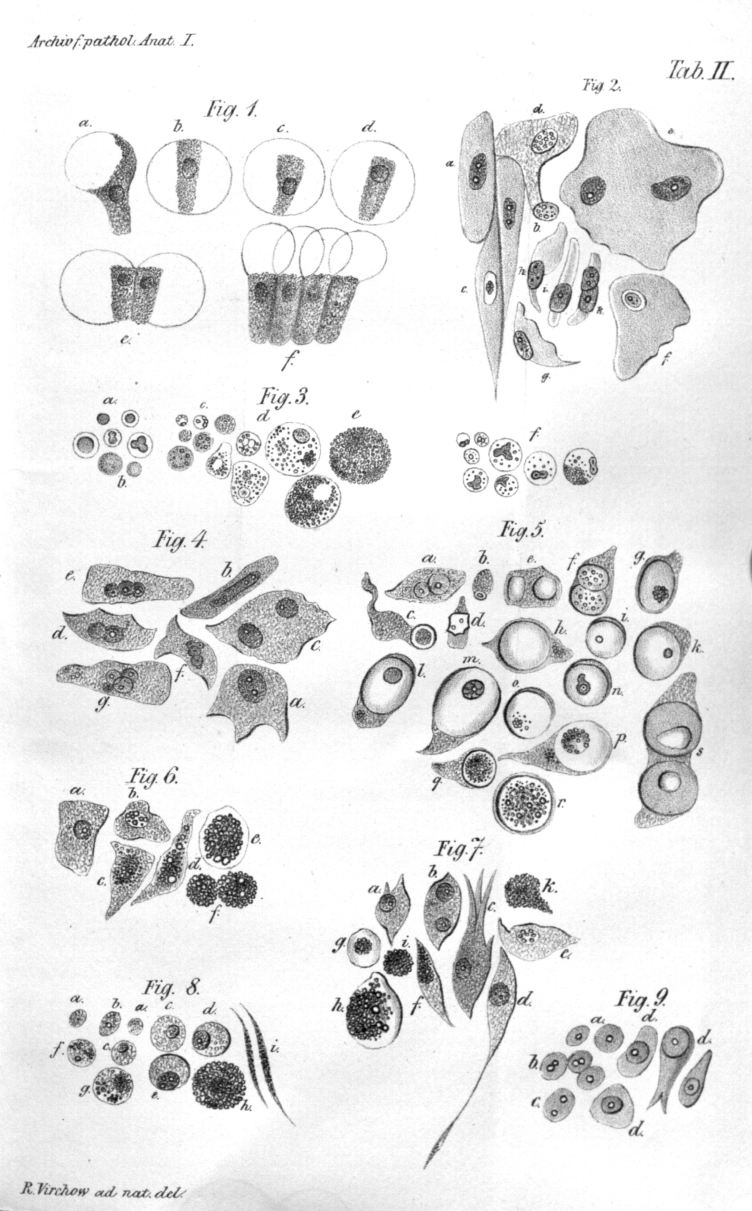
\includegraphics{figures/intro/virchow.png}
\caption[Illustration du livre « Cell theory » de Rudolf Virchow]{\label{fig:virchow}Illustration
du livre « Cell theory » de Rudolf Virchow (Virchow,
\hyperref[ref-virchow1860cellular]{1860})}
\end{figure}

C'est véritablement au 20ème siècle que toute la complexité de la
cellule se dévoile à nous grâce à l'apparition de nombreuses avancées
technologiques telle que la découverte de l'ADN (Watson et al.,
\hyperref[ref-watson1953molecular]{1953}), l'apparition de la biologie
moléculaire ainsi que la création de microscopes toujours plus précis.

Ce travail de thèse a pour objectif l'étude d'une phase tout à fait
cruciale durant la vie d'une cellule: le moment où elle se divise. Cette
étape, appelée la mitose, permet selon le second axiome de la théorie
cellulaire, le maintien de l'intégrité cellulaire tout au long des
générations.

La mitose est un domaine de recherche important pour deux raisons
majeures :

\begin{itemize}
\tightlist
\item
  Mieux comprendre le fonctionnement du vivant par la compréhension de
  ce mécanisme primordial sans lequel la vie ne serait jamais apparue
  sur Terre.
\item
  Mieux comprendre le cancer, qui n'est autre qu'un ensemble de maladies
  impliquant un dérèglement de la division cellulaire.
\end{itemize}

Mais avant de comprendre comment une cellule se divise, replaçons ce
processus de division dans un contexte plus large qui consiste à
déchiffrer les différentes étapes de la vie d'une cellule.

\section{La vie d'une cellule}\label{la-vie-dune-cellule}

Comme le disait François Jacob en 1974, \emph{« The dream of every cell
is to become two cells. »}. Et quand elle n'essaie pas de devenir deux
cellules, elle prépare tout afin que la division se déroule
correctement. L'ensemble de ces processus qui dicte la vie d'une cellule
est un cycle qui se répète depuis longtemps maintenant : le cycle
cellulaire.

Le cycle cellulaire est l'ensemble des étapes qui composent la vie d'une
cellule. Cette série d'événements varie de manière considérable d'une
cellule à une autre. Le cycle cellulaire dépend de l'identité de la
cellule (principalement définie par son matériel génétique) ainsi que de
son contexte écologique; c'est à dire le milieu environnant dans lequel
elle se trouve.

Malgré son incroyable diversité, on peut diviser le cycle cellulaire en
deux grandes étapes communes à l'ensemble des organismes. Une étape de
croissance appelée l'interphase ainsi qu'une étape de division appelée
la mitose.

C'est durant l'interphase que la cellule va passer la plupart de son
existence (Figure~\ref{fig:cycle}). Celle-ci est composée de plusieurs
sous-étapes (Norbury and Nurse, \hyperref[ref-Norbury1992]{1992}):

\begin{itemize}
\item
  une phase de croissance (\textbf{phase G1}) durant laquelle la cellule
  va augmenter sa taille ainsi que son volume cellulaire. C'est aussi
  durant cette période qu'elle va synthétiser l'ensemble des protéines
  spécifiques à son identité ainsi qu'en réponse au milieu dans lequel
  elle se trouve.
\item
  une phase de synthèse (\textbf{phase S}) durant laquelle la cellule va
  répliquer son matériel génétique, l'ADN. La duplication des
  chromosomes est une étape cruciale pour le maintien de la stabilité
  génétique. En effet chacun des nucléotides (allant de quelques
  milliers à plusieurs milliards selon le type de cellules) doit être
  dupliqué avec une grande précision afin que les deux cellules filles
  se voient transmettre la même information génétique.
\item
  une phase de préparation de la division cellulaire (\textbf{phase G2})
  durant laquelle la cellule relance la synthèse de protéine et croît
  rapidement afin de préparer sa division. Cette phase est importante
  car elle possède un système de blocage du cycle cellulaire (aussi
  appelé « checkpoint » ou « point de contrôle ») qui permet de retarder
  l'entrée en mitose en cas de problème de réplication de l'ADN apparu
  en phase S.
\item
  la phase de division (\textbf{mitose} ou \textbf{phase M}) qui fait
  suite à l'interphase est l'étape durant laquelle la cellule se divise
  en deux cellules filles.
\end{itemize}

\begin{figure}[htbp]
\centering
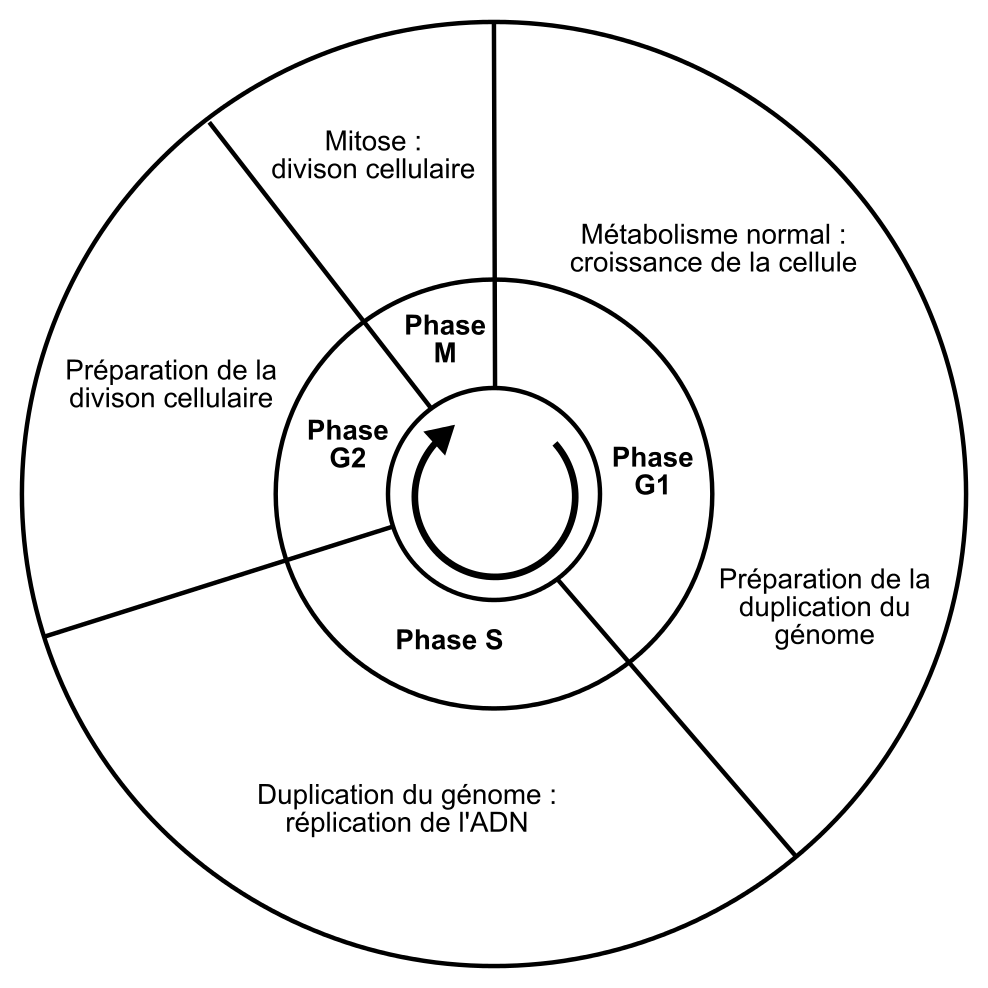
\includegraphics{figures/intro/cycle.png}
\caption[Les différentes étapes du cycle cellulaire]{\label{fig:cycle}Les
différentes étapes du cycle cellulaire. Les phases S et G2 préparent la
division cellulaire qui a lieu à la phase M.}
\end{figure}

Il est important de souligner que dans la réalité, il existe autant de
cycles cellulaires différents qu'il existe de type de cellules. Donc
malgré la conservation de certains mécanismes primordiaux, chaque type
de cellules possède son propre cycle cellulaire (Lodish et al.,
\hyperref[ref-Lodish2000]{2000}; Norbury and Nurse,
\hyperref[ref-Norbury1992]{1992}).

D'une manière plus générale on peut aussi noter que l'un des enjeux de
la biologie cellulaire aujourd'hui est de comprendre quelle est la part
des mécanismes conservée entre différents types cellulaires et quelle
est la part spécifique de l'organisme étudié.

La dernière phase du cycle cellulaire est donc la mitose, c'est à dire
le moment où une cellule va devenir deux cellules.

\section{La mitose : la dernière étape du cycle
cellulaire}\label{la-mitose-la-derniuxe8re-uxe9tape-du-cycle-cellulaire}

La dernière étape du cycle cellulaire est la mitose. Durant cette étape
la cellule mère va se diviser en deux cellules filles. Tous les
mécanismes précédents et ceux composant la mitose ont pour objectif
d'assurer une division intègre et égale entre les deux cellules filles.

L'entrée en mitose est un événement contrôlé en grande partie par la
kinase Cdc2 aussi appelée Cdk1 (Nasmyth and Reed,
\hyperref[ref-Nasmyth1980]{1980}; Nurse and Thuriaux,
\hyperref[ref-Nurse1980]{1980}). Cette protéine, conservée de la levure
à l'Homme, s'associe avec une protéine régulatrice, la Cycline B. Le
complexe s'active alors de manière transitoire pour former le fuseau
mitotique.

\subsection{Les phases de la mitose}\label{les-phases-de-la-mitose}

De manière étonnante, la mitose est un processus relativement bien
conservé chez la majorité des cellules eucaryotes. Les grandes phases la
composant peuvent donc être décrites de manière commune pour un grand
nombre d'organismes, allant de la cellule humaine aux eucaryotes
unicellulaires comme la levure.

Cette étape cruciale du cycle cellulaire est d'autant plus importante
que des défauts durant ce processus peuvent être à l'origine de cellules
possédant un nombre défectueux de chromosomes (cellule aneuploïde). On
sait aussi que les cellules aneuploïdes peuvent contribuer à la
formation de tumeur cancéreuse (Kops et al.,
\hyperref[ref-Kops2005]{2005}).

Les différentes phases de la mitose sont (Figure~\ref{fig:mitosis}) :

\begin{itemize}
\tightlist
\item
  la \textbf{prophase} : les brins d'ADN (la chromatine) se condensent
  pour former des structures ordonnées et séparées les unes des autres;
  les chromosomes. Les deux pôles, appelés centrosomes chez les
  eucaryotes supérieurs, se séparent afin de former le fuseau mitotique.
\end{itemize}

Note: certains fuseaux mitotiques sont formés en l'absence de pôles
(\emph{« acentrosomal spindle formation »} en anglais). Ce type de
division très particulier ne sera pas discuté dans ce manuscrit.

\begin{itemize}
\item
  la \textbf{prométaphase} : la membrane nucléaire se désassemble dans
  le cas d'une mitose ouverte (Boettcher and Barral,
  \hyperref[ref-Boettcher2013]{2013}) tandis qu'elle reste intacte dans
  les mitoses fermées (répandues chez les protistes et organismes
  unicellulaires). Les chromosomes s'attachent aux microtubules par
  l'intermédiaire d'une structure protéique qui s'assemble au même
  moment au niveau du centromère des chromosomes: le kinétochore.
\item
  la \textbf{métaphase} : les chromosomes alors attachés aux pôles par
  l'intermédiaire des microtubules viennent se positionner à l'équateur
  de la cellule pour former la plaque métaphasique. Cette étape cruciale
  de la mitose est régulée par des points de contrôle qui détectent la
  présence de chromosomes mal attachés et retardent le passage à l'étape
  suivante.
\end{itemize}

En effet, la transition métaphase/anaphase est régulée par un point de
contrôle appelé le SAC (Spindle Assembly Checkpoint) qui permet à la
cellule de bloquer la ségrégation des chromosomes en cas d'attachement
incorrect (Musacchio and Salmon, \hyperref[ref-Musacchio2007]{2007}).
L'anaphase débute au moment de l'activation de l'APC (Anaphase Promoting
Complex), une ubiquitine ligase responsable de la dégradation de la
Cyclin B et donc de l'inactivation du complexe Cdk1 (Sivakumar and
Gorbsky, \hyperref[ref-Sivakumar2015]{2015}).

\begin{itemize}
\item
  l'\textbf{anaphase} : durant l'anaphase A et grâce à l'activation de
  l'APC, le complexe cohésine reliant les chromatides sœurs est dégradé
  (Oliveira et al., \hyperref[ref-Oliveira2010]{2010}). Cela conduit au
  mouvement de chaque chromatide vers son pôle respectif grâce à la
  dépolymérisation des microtubules au cours de l'anaphase A. A
  l'anaphase B, le fuseau mitotique s'allonge, éloignant alors les pôles
  du fuseau et les chromosomes loin du centre de la cellule. On notera
  que ces deux phases peuvent être distinctes ou pas selon le type de
  cellule étudiée.
\item
  la \textbf{télophase} : les microtubules attachés aux kinétochores se
  désagrègent, les chromosomes se décondensent et retournent à leur état
  initial de brins d'ADN. L'enveloppe nucléaire se reforme dans le cas
  d'une mitose ouverte.
\item
  la \textbf{cytocinèse} : à ce stade, la mitose est finie. Durant cette
  période, la cellule va alors se diviser grâce à la formation d'un
  sillon au niveau de la membrane cytoplasmique qui s'invagine jusqu'à «
  couper » la cellule mère en deux cellules filles.
\end{itemize}

\begin{figure}[htbp]
\centering
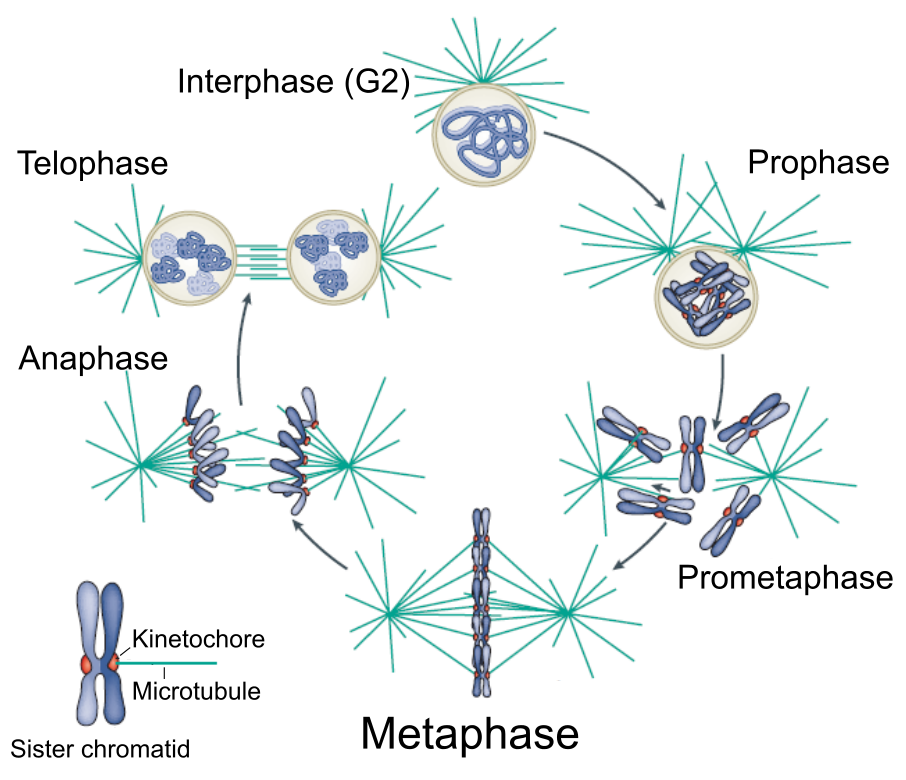
\includegraphics{figures/intro/mitosis.png}
\caption[Les différentes étapes de la mitose]{\label{fig:mitosis}Les
différentes étapes de la mitose (adapté de Cheeseman and Desai
(\hyperref[ref-Cheeseman2008]{2008})). Durant les cinq phases de la
mitose la cellule établit un fuseau mitotique par élongation de ces deux
pôles (en vert) puis doit répartir la même quantité de chromosomes (en
bleu) à chacun des pôles.}
\end{figure}

On voit bien à travers la description des différentes étapes de la
mitose que l'une des caractéristiques essentielles des chromosomes
durant la mitose est leur capacité à se mouvoir dans la cellule de façon
coordonnée à la fois dans le temps et dans l'espace.

Nous allons à présent voir qu'un grand nombre d'acteurs sont nécessaires
afin de produire et réguler ce mouvement.

\subsection{Le kinétochore}\label{le-kinuxe9tochore}

Le kinétochore est un assemblage de protéines de très grande taille
(jusqu'à 80 chez les cellules humaines) dont l'assemblage se situe sur
la partie centromérique des chromatides au niveau des variants d'histone
H3 (appelé CENP-A).

Il est composé de deux régions (Figure~\ref{fig:kt}) :

\begin{itemize}
\item
  \textbf{la plaque interne} qui s'associe de manière très spécifique
  avec la chromatine centromérique par l'intermédiaire entre autre de
  l'histone CENP-A.
\item
  \textbf{la plaque externe}, épaisse de 50 à 60nm qui est responsable
  des interactions avec le fuseau mitotique, notamment les microtubules
  kinétochoriens. Cette région possède des sites d'ancrage pour les
  microtubules permettant le mouvement des chromosomes durant la mitose.
  Le nombre de site d'ancrage varie fortement d'une espèce à une autre
  allant d'une quarantaine chez l'humain à seulement un site
  d'attachement pour la levure à bourgeon (\emph{S. cerevisiae}).
\end{itemize}

\begin{figure}[htbp]
\centering
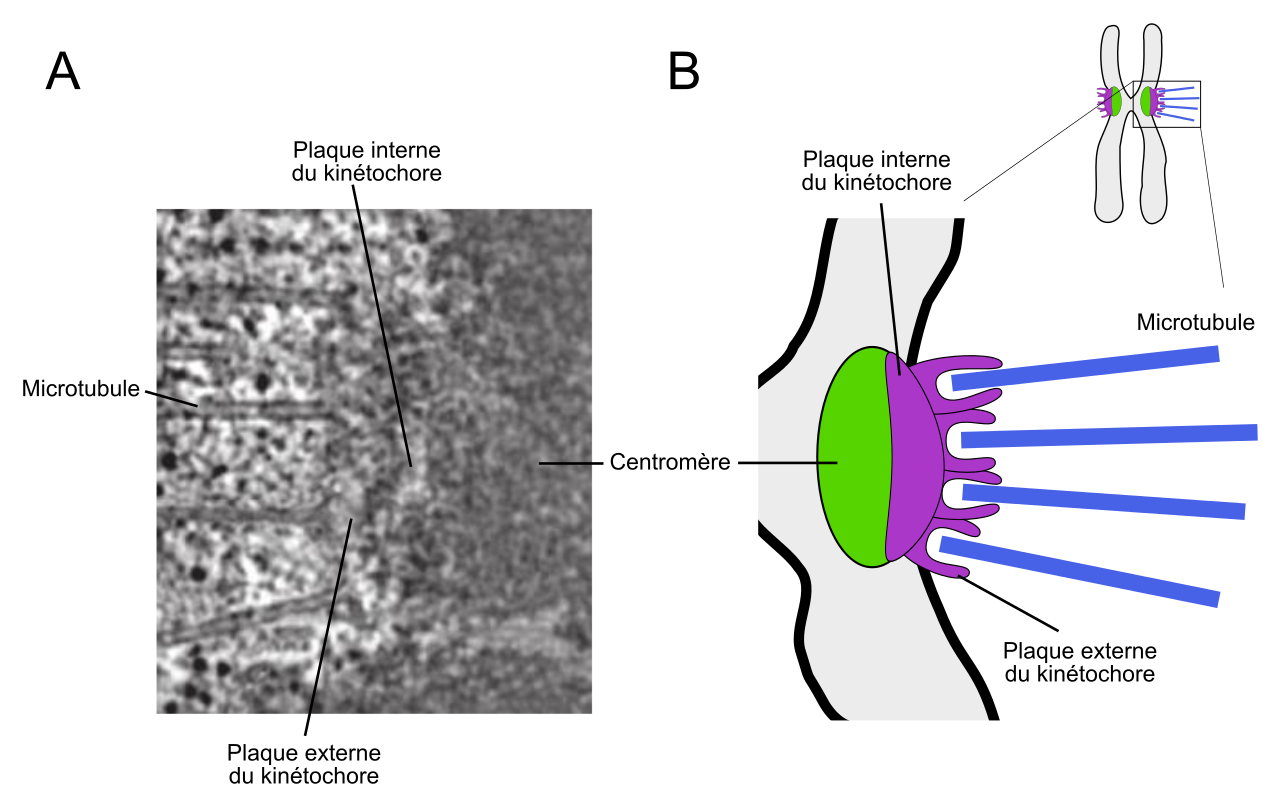
\includegraphics{figures/intro/kt.png}
\caption[Structure d'un kinétochore]{\label{fig:kt}Structure d'un
kinétochore. \textbf{A.} Vue d'un kinétochore humain de côté par
microscopie électronique (McEwen et al.
(\hyperref[ref-McEwen2007]{2007})). \textbf{B.} Schéma des différentes
plaques d'un kinétochore}
\end{figure}

Le kinétochore s'assemble durant la prométaphase et joue plusieurs rôles
importants. En plus d'être un acteur essentiel dans le bon déroulement
du point de contrôle de la transition métaphase/anaphase (le SAC), il
joue aussi un rôle structurel dans l'attachement entre le chromosome et
les microtubules.

\subsection{Les microtubules}\label{les-microtubules}

Les microtubules sont l'un des constituants majeurs du cytosquelette. Ce
sont des structures de forme tubulaire d'un diamètre de 20nm et d'une
longueur très variable pouvant aller jusqu'à plusieurs micromètres. Ils
sont formés de dimères de tubuline, eux mêmes composés de deux sous
unités, la tubuline α et la tubuline β.

La formation d'un microtubule requiert un complexe protéique qui jouera
le rôle de patron de construction, constitué de la γ tubuline. Celui-ci
forme un anneau permettant la disposition de chaque protofilament tel
que présenté Figure~\ref{fig:mt}A. L'extrémité + est coiffée de dimère
GTP et c'est son hydrolyse en GDP qui permet l'assemblage des
protofilaments.

Par ailleurs, le microtubule est un polymère extrêmement dynamique dont
les extrémités passent leur temps à basculer entre deux états : la
polymérisation et la dépolymérisation (voir Figure~\ref{fig:mt}B). Les
deux extrémités étant chargées différemment en GTP et GDP, elles
possèdent une dynamique plus ou moins importante. On parle d'extrémité
plus pour celle chargée en GTP et donc très dynamique (coiffée par la
tubuline β) et d'extrémité moins pour celle chargée en GDP donc moins
dynamique (coiffée par la tubuline α).

\begin{figure}[htbp]
\centering
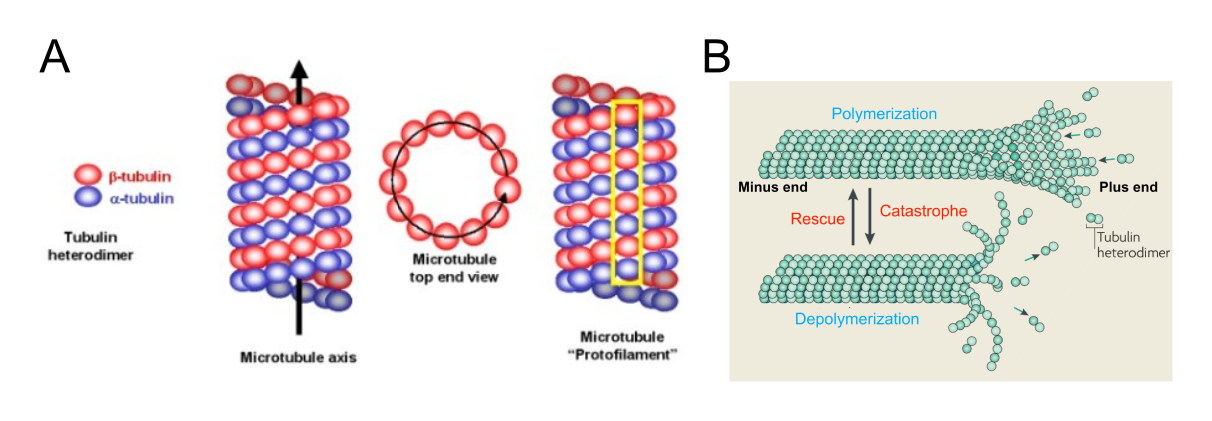
\includegraphics{figures/intro/mt.png}
\caption[Structure et dynamique du microtubule]{\label{fig:mt}Structure
et dynamique du microtubule. \textbf{A.} Schéma présentant
l'organisation d'un microtubule. \textbf{B.} Les microtubules sont des
structures hautement dynamiques qui passent très souvent d'un état à un
autre (Walczak et al., \hyperref[ref-Walczak2010]{2010}).}
\end{figure}

Les microtubules, et d'une manière plus générale l'ensemble des
protéines du cytosquelette, permettent le maintien de la forme
tridimensionnelle. De plus, elles participent aussi de manière active au
processus de migration cellulaires ainsi que de transport
intra-cellulaire. C'est ainsi qu'il est possible d'apprécier la grande
diversité de formes et d'élasticité des cellules composant l'ensemble
des organismes connus.

Les microtubules sont aussi connus pour leur rôle dans le transport
cytoplasmique de divers composants tels que des vésicules ou autres
grandes protéines. En effet leur polarité et leur grande rigidité
permettent un déplacement sur de longues distances et de manière
dirigée. Par exemple, les neurones contiennent un grand nombre de
microtubules nécessaires aux déplacements de nombreuses protéines soit
vers les prolongements cellulaires ou bien vers le corps cellulaire.

Le transport est rendu possible grâce à des protéines associées aux
microtubules (appelées Microtubules-Associated Proteins ou MAPs en
anglais). Par exemple, les moteurs moléculaires sont des MAPs très
connus et étudiés. Parmi eux, les kinésines se déplacent vers
l'extrémité plus tandis que les dynéines se déplacent vers l'extrémité
moins des microtubules.

Enfin le rôle des microtubules dans la mobilité cellulaire est aussi
très étudié. Ce sont par exemple les composants majeurs de l'axonème qui
forment les flagelles des cellules eucaryotes (spermatozoïdes et
certains protistes).

Pour finir, on soulignera leur importance capitale durant la mitose car
ce sont eux qui forment l'essentiel du fuseau mitotique. En plus d'un
rôle structurel durant la division cellulaire, ils participent aussi de
manière active en fournissant une partie de l'énergie nécessaire au
déplacement des chromosomes.

Bien que les microtubules soient des structures très dynamiques, un
grand nombre de molécules et de protéines sont capables de modifier
cette dynamicité. Notamment, une famille de protéines est connue pour
induire la dépolymérisation des microtubules pendant la mitose.

\subsection{Les kinésines dépolymérisatrices des
microtubules}\label{les-kinuxe9sines-duxe9polymuxe9risatrices-des-microtubules}

Les premières études sur cette famille de kinésines ont commencé dans
les années 1990 (voir la revue à propos de cette famille de kinésine par
Claire E. Walczak (Walczak et al., \hyperref[ref-Walczak2013a]{2013})).
La kinésine-13 fut la première à être décrite comme une kinésine
dépolymérisatrice des microtubules. Par exemple, la déplétion de la
kinésine-13 dans des extraits d'œufs de \emph{Xenopus} (appelé XKCM1) a
pour effet d'augmenter la taille des microtubules qui présentent par
ailleurs un taux de catastrophe plus bas (Walczak et al.,
\hyperref[ref-Walczak1996]{1996}). Par la suite la kinésine-13 a été
retrouvée dans de nombreux organismes pour lesquels il a été montré un
rôle dans la déstabilisation des microtubules (Ganem et al.,
\hyperref[ref-Ganem2005]{2005}; Maney and Hunter,
\hyperref[ref-Maney1998]{1998}).

Étonnamment personne ne retrouva la kinésine-13 chez les champignons et
c'est au début des années 2000 que la kinésine-8 fut décrite chez la
levure. Chez la levure à fission (\emph{Schizosaccharomyces pombe}), la
déplétion de la kinésine-8 (Klp5 et Klp6) entraîne un allongement des
microtubules cytoplasmiques ainsi qu'un défaut dans l'alignement des
chromosomes en métaphase (Garcia et al.,
\hyperref[ref-Garcia2002d]{2002}; West et al.,
\hyperref[ref-West2002]{2002}). Tandis que chez la levure à bourgeon
(\emph{Saccharomyces cerevisiae}), les cellules mutantes pour la
kinésine-8 (Kip3) présentent un défaut de positionnement du noyau
(Cottingham and Hoyt, \hyperref[ref-Cottingham1997]{1997}). D'une
manière plus générale, de nombreuses études ont montré que la kinésine-8
est localisée à l'extrémité plus des microtubules kinétochoriens et que
sa délétion entraîne un allongement du fuseau mitotique, un décentrage
des chromosomes ainsi qu'un délai d'entrée en anaphase dû à l'activation
du SAC (Goshima et al., \hyperref[ref-Goshima2005]{2005}; Jaqaman et
al., \hyperref[ref-Jaqaman2010]{2010}; Mayr et al.,
\hyperref[ref-Mayr2007]{2007}; Stumpff et al.,
\hyperref[ref-Stumpff2008]{2008}; Wargacki et al.,
\hyperref[ref-Wargacki2010]{2010}).

Une étude phylogénique suggère que la majorité des cellules eucaryotes
possèdent au moins un gène codant pour l'une des deux kinésines
dépolymérisatrices (Wickstead and Gull,
\hyperref[ref-Wickstead2006]{2006}). Il a même été montré qu'un parasite
protozoaire (\emph{Theileria annulata}) ne possède que deux kinésines:
la kinésine-8 et la kinésine-13. Tout ceci révèle l'importance
fondamentale qu'ont ces kinésines dépolymérisatrices dans la dynamique
des microtubules.

Par ailleurs, l'analyse de la structure 3D de ces deux kinésines (Ogawa
et al., \hyperref[ref-Ogawa2004]{2004}; Peters et al.,
\hyperref[ref-Peters2010]{2010}) montre une très forte similarité dans
l'agencement spatial des brins et des hélices les composant
(Figure~\ref{fig:dep_kinesin}), ce qui suggère des activités
catalytiques similaires.

\begin{figure}[htbp]
\centering
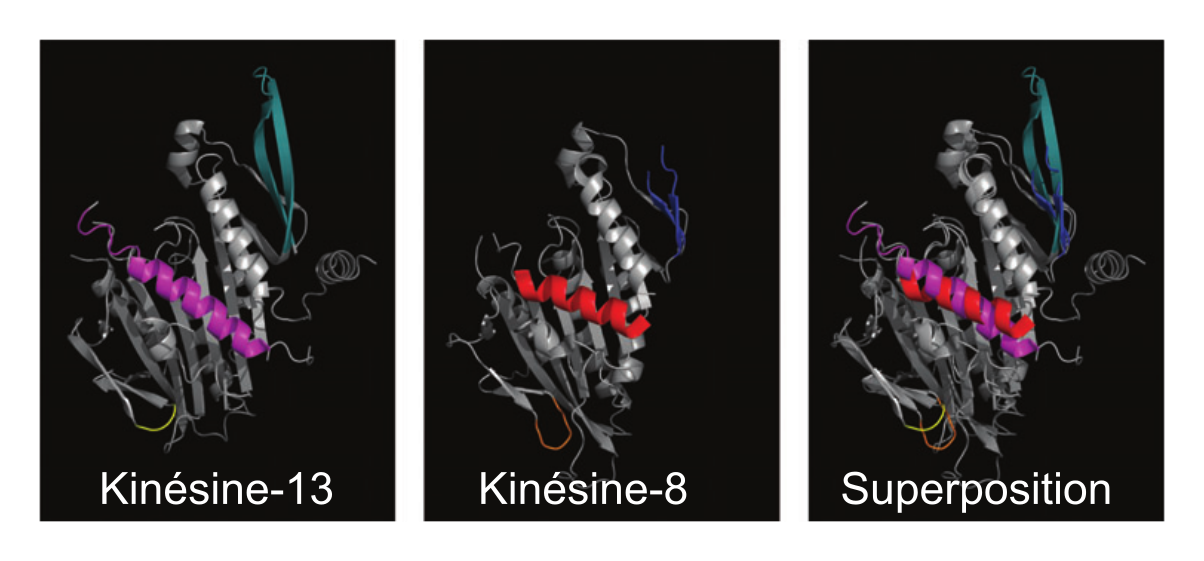
\includegraphics{figures/intro/dep_kinesin.png}
\caption[Reconstruction 3D des kinésines dépolymérisatrice]{\label{fig:dep_kinesin}Vue
en trois dimensions de la kinésine-13 (MCAK) et de la kinésine-8
(Kif18a) chez des cellules humaines. La troisième vue montre une
superposition des deux protéines. (Walczak et al.,
\hyperref[ref-Walczak2013a]{2013})}
\end{figure}

On notera aussi la grande conservation des domaines protéiques qui
composent la kinésine-8 chez un grand nombre d'organismes modèles
(cellule humaine, levure à bourgeon, levure à fission, cellule de
drosophile) comme le montre la Figure~\ref{fig:proteicdomain}.

\begin{figure}[htbp]
\centering
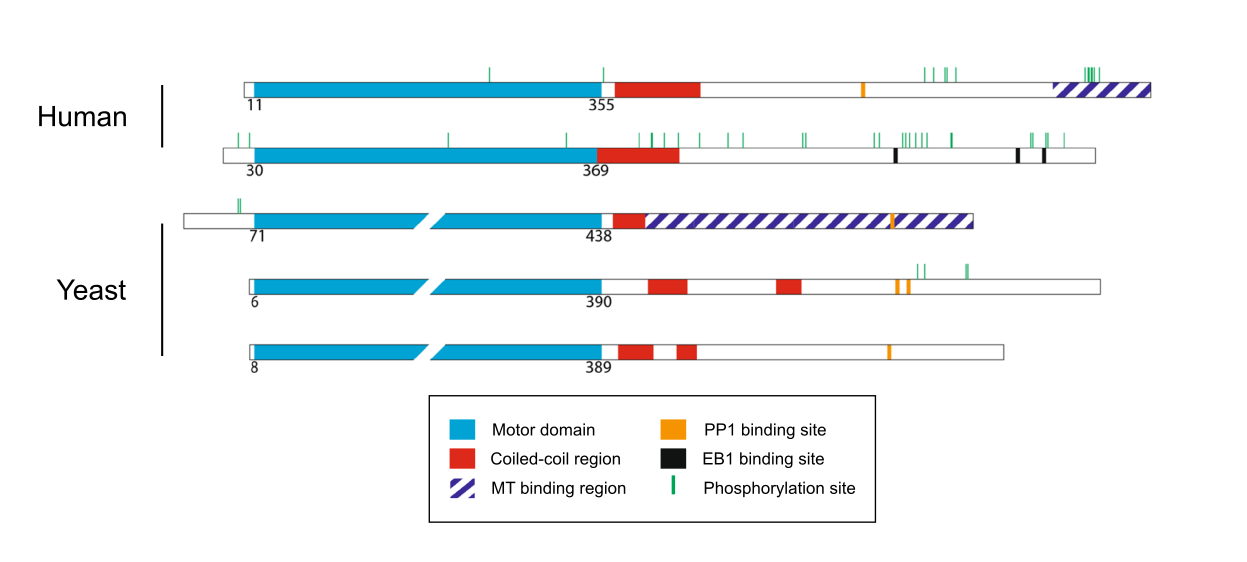
\includegraphics{figures/intro/proteicdomain.png}
\caption[Les domaines protéiques des différentes kinésine-8]{\label{fig:proteicdomain}Vue
schématique des domaines protéiques composant la kinésine-8 chez la
cellule humaine, la levure à bourgeon et la levure à fission (Messin and
Millar, \hyperref[ref-Messin2014]{2014}).}
\end{figure}

Si les protéines dépolymérisatrices influencent le comportement de
l'attachement entre le microtubule et le kinétochore, il n'a pas été
montré qu'elle joue un rôle dans l'attachement. Celui-ci dépend de
protéines spécifiques du kinétochore qui permettent l'ancrage du
microtubule, ainsi que le maintien de l'attachement.

\subsection{L'ancrage du microtubule au
kinétochore}\label{lancrage-du-microtubule-au-kinuxe9tochore}

Durant la mitose, les microtubules attachent les chromosomes par
l'intermédiaire d'une grande structure protéique appelée le kinétochore.
L'attache se situe au niveau de la plaque externe du kinétochore et est
principalement réalisée grâce au complexe NDC80 (DeLuca et al.,
\hyperref[ref-DeLuca2002]{2002}, \hyperref[ref-DeLuca2006]{2006};
McCleland et al., \hyperref[ref-McCleland2004]{2004}; Wigge and
Kilmartin, \hyperref[ref-Wigge2001]{2001}).

Ce complexe est un hétérotétramère composé des protéines : Ndc80, (Hec1
chez les humains), Nuf2, Spc24 et Spc25 (Wei et al.,
\hyperref[ref-Wei2005]{2005}) (voir Figure~\ref{fig:ndc80}A). L'une des
extrémités qui possède un domaine pouvant s'attacher au microtubule est
composée de Ndc80-Nuf2 tandis que l'autre extrémité, Scp25-Spc24,
possède un domaine s'attachant à la plaque externe du kinétochore.

Chez la levure un autre complexe protéique, appelé Dam1 ou DASH, a été
décrit comme participant à l'attachement KT-MT. Ce complexe forme un
oligomère autour du MT en forme d'anneau partiel ou complet (Miranda et
al., \hyperref[ref-Miranda2005]{2005}; Westermann et al.,
\hyperref[ref-Westermann2006]{2006}).

\begin{figure}[htbp]
\centering
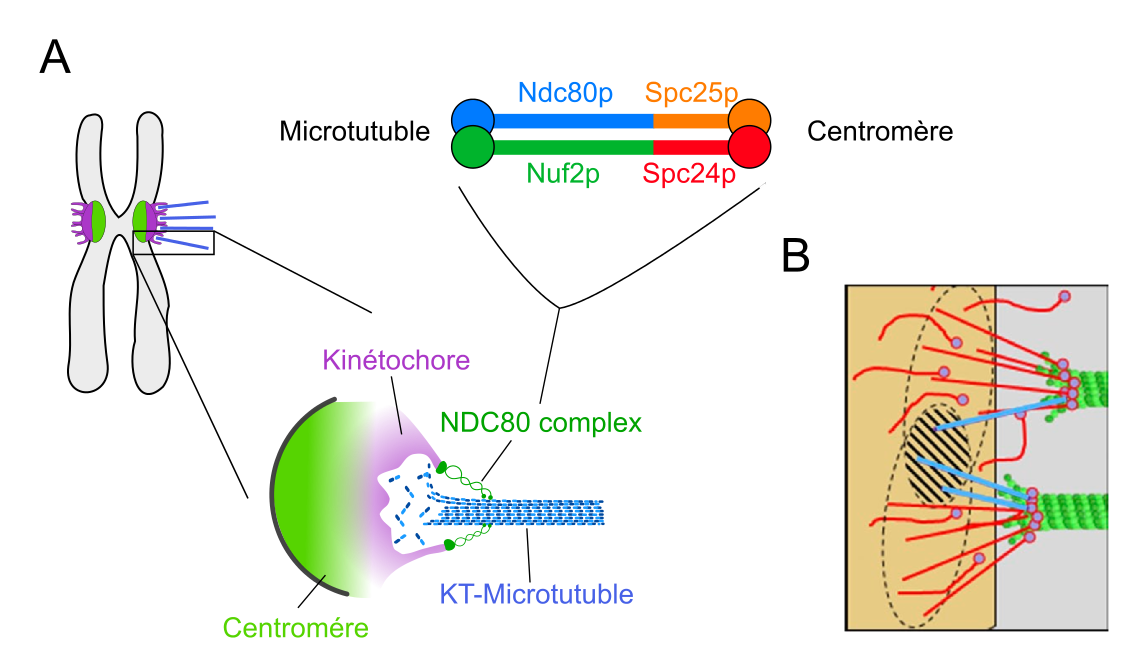
\includegraphics{figures/intro/ndc80.png}
\caption[Stucture de l'attachement kinétochore-microtubule]{\label{fig:ndc80}Stucture
de l'attachement kinétochore-microtubule. \textbf{A.} Vue schématique de
la structure du complexe NDC80 ainsi que sa localisation dans le
kinétochore. \textbf{B.} Interaction non contrainte entre des complexes
NDC80 (en rouge) avec différents microtubules (en vert) (Zaytsev et al.,
\hyperref[ref-Zaytsev2014]{2014}).}
\end{figure}

Plus récemment J.G DeLuca et al. ont proposé un modèle continu de
l'attachement des microtubules au kinétochore (Zaytsev et al.,
\hyperref[ref-Zaytsev2014]{2014}). En effet les sites d'attachement ne
sont plus vus comme un ensemble d'éléments discrets, mais comme une
surface sur laquelle les attachements se font de manière non exclusive
(voir Figure~\ref{fig:ndc80}B).

\subsection{Les différents types
d'attachements}\label{sec:attachments-type}

L'association des kinétochores frères avec leurs pôles respectifs
s'appelle un attachement amphitélique, on parle aussi de chromosomes
biorientés (voir Figure~\ref{fig:attachements}). Il a été montré que les
erreurs d'attachement sont fréquentes en prométaphase et qu'elles sont
pour la plupart corrigées avant le début de la séparation des
chromosomes, l'anaphase.

On distingue trois types d'erreurs dans les attachements KT-MT (voir
Figure~\ref{fig:attachements}):

\begin{itemize}
\item
  \textbf{monotélique} : seulement un des deux kinétochores est attaché
  à des MTs provenant tous du même pôle.
\item
  \textbf{syntélique} : les deux kinétochores sont associés à des MTs
  provenant du même pôle.
\item
  \textbf{mérotélique} : un kinétochore est associé à des MTs provenant
  des deux pôles à la fois.
\end{itemize}

\begin{figure}[htbp]
\centering
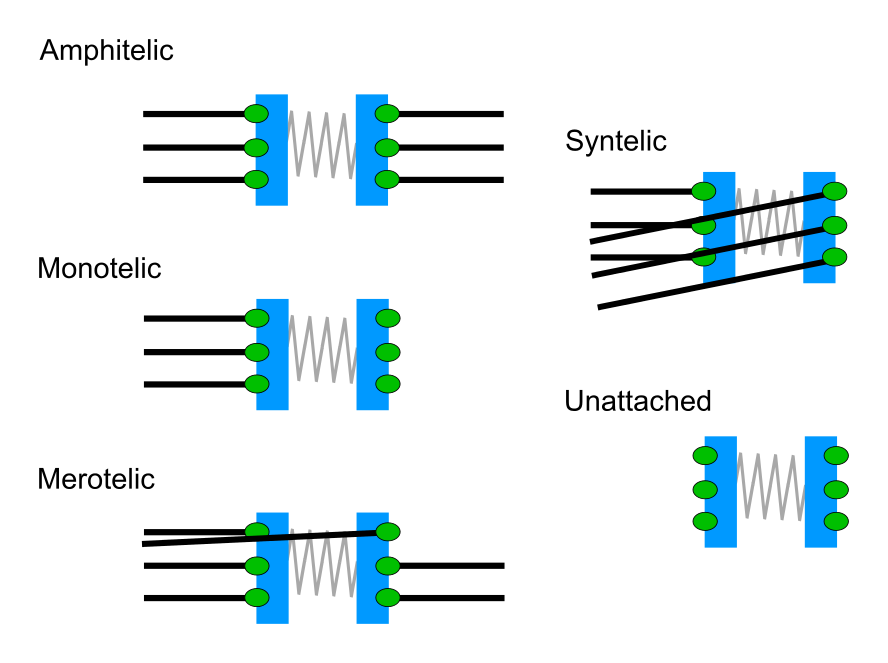
\includegraphics{figures/intro/attachments.png}
\caption[Les différents types d'attachements des microtubules aux kinétochores]{\label{fig:attachements}Les
différents types d'attachements des microtubules aux kinétochores. Le
seul attachement correct pour le fuseau mitotique est l'attachement
amphitélique aussi appelé attachement bi-orienté. Les autres
attachements sont généralement corrigés durant la mitose.}
\end{figure}

Un attachement incorrect des kinétochores durant l'anaphase peut
entraîner une perte de chromosome et par la suite la mort cellulaire ou
bien la dégénérescence d'un tissu. La cellule a donc développé des
mécanismes robustes de correction.

D'abord de manière purement géométrique, suite au processus de
réplication et de condensation, les deux kinétochores sœurs sont placés
dos à dos dans des directions opposées. Il en résulte que si l'un des
kinétochores est accroché à un pôle, l'autre kinétochore sera alors plus
susceptible de s'associer avec le pôle opposé.

Dans les années 90, Nicklas et al. montra dans un expérience de
micromanipulation sur des chromosomes de spermatocyte de sauterelle, que
l'attachement KT-MT est par nature instable et qu'il se stabilise à
mesure que la tension augmente (Nicklas et al.,
\hyperref[ref-Nicklas1982]{1982}).

Par ailleurs, des expériences de microdissection au laser sur des
chromosomes en métaphase (Skibbens et al.,
\hyperref[ref-Skibbens1995]{1995}) ont montré que les deux chromatides
sœurs se déplacent vers leurs pôles respectifs après ablation de leur
région centrale, ce qui indique que l'attachement d'un microtubule à un
kinétochore produit une force dans la direction du pôle qui attache le
microtubule. Par conséquent, un chromosome amphitélique, correctement
attaché, est nécessairement sous tension tandis que les attachements
monotéliques ou syntéliques doivent subir une tension plus faible. Ainsi
les attachements incorrects devraient être éliminés avec le temps tandis
que les attachements corrects auraient tendance à être maintenus
jusqu'au début de l'anaphase (Kirschner and Mitchison,
\hyperref[ref-Kirschner1986]{1986}).

Un des mécanismes proposés pour expliquer l'instabilité des attachements
incorrects, sous une moindre tension, est basé sur l'activité d'une
protéine kinase appelée Aurora B et localisée au centre du centromère.
La phosphorylation de certaines protéines du kinétochore par Aurora B
réduit l'affinité de l'attachement (DeLuca et al.,
\hyperref[ref-DeLuca2006]{2006}). Comme présenté sur la
Figure~\ref{fig:aurora}, si la distance entre les deux kinétochores est
grande, due à une tension élevée, Aurora B n'aurait pas accès aux
protéines du kinétochore et ne pourrait donc pas déstabiliser
l'attachement en déphosphorylant ces substrats (Tanaka et al.,
\hyperref[ref-Tanaka2002]{2002}).

\begin{figure}[htbp]
\centering
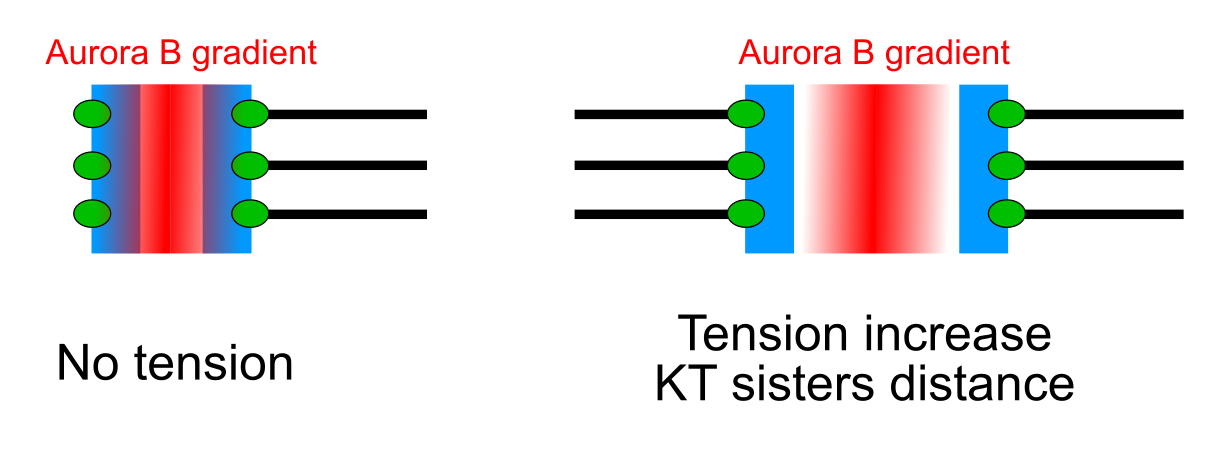
\includegraphics{figures/intro/aurora.png}
\caption[Le mécanisme de déstabilisation de l'attachement KT-MT]{\label{fig:aurora}Le
mécanisme de déstabilisation de l'attachement KT-MT. Quand les deux
kinétochores sœurs sont éloignés (schéma de droite), Aurora B ne peut
pas atteindre les protéines du kinétochore (en vert) et donc
déstabiliser l'attachement KT-MT.}
\end{figure}

Ces mécanismes ne peuvent néanmoins pas corriger les attachements
mérotéliques. En effet les deux kinétochores étant partiellement
attachés aux deux pôles, le fuseau exerce quand même une tension à
travers le centromère. Le déséquilibre de tension se situe alors au
niveau du kinétochore. Bien que ces mécanismes de correction soient
encore mal compris, l'un d'entre eux semble impliquer Aurora B (Cimini
et al., \hyperref[ref-Cimini2006]{2006}). Un autre mécanisme propose une
correction structurelle en provoquant un déséquilibre de force présent
en anaphase sur le kinétochore mérotélique et implique les forces
responsable de l'élongation du fuseau (Courtheoux et al.,
\hyperref[ref-Courtheoux2009]{2009}).

Les mécanismes en charge de l'intégrité et de la correction des
attachements des chromosomes prennent du temps. La cellule a donc
développé un point de contrôle afin de mettre la mitose « en pause »
avant l'entrée en anaphase, afin que tous les attachements puissent être
corrigés.

\section{La métaphase : point d'orgue de la division
cellulaire}\label{la-muxe9taphase-point-dorgue-de-la-division-cellulaire}

La métaphase correspond au moment où l'ensemble des chromatides sœurs
sont encore attachées entre elles par la cohésine et alignées au milieu
du fuseau mitotique entre les deux pôles
(Figure~\ref{fig:spindle_micro}).

\begin{figure}[htbp]
\centering
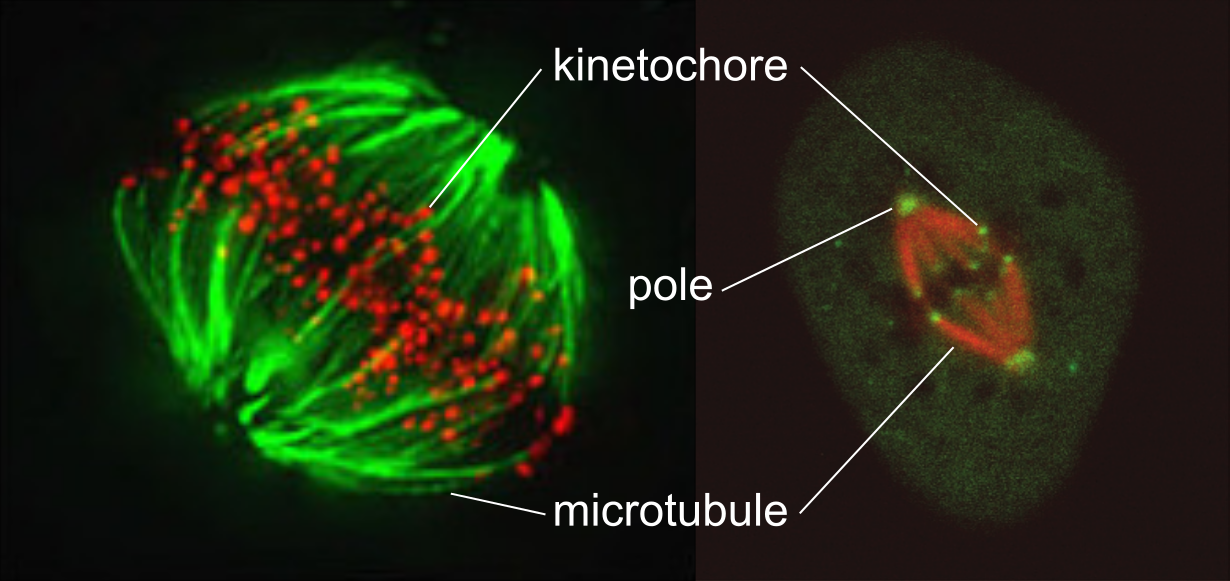
\includegraphics{figures/intro/spindle_micro.png}
\caption[Deux types de cellules différentes en métaphase]{\label{fig:spindle_micro}Deux
cellules en métaphase (cellule HeLa à gauche et cellule Ptk1 à droite).
Pour les deux cellules les kinétochores de l'ensemble des chromosomes
sont marqués respectivement en rouge et vert tandis que les microtubules
sont marqués respectivement en vert et rouge. (Huang et al.,
\hyperref[ref-Huang2008]{2008}; Wan et al.,
\hyperref[ref-Wan2012]{2012})}
\end{figure}

\subsection{La congression des
chromosomes}\label{la-congression-des-chromosomes}

L'étape d'alignement des chromosomes aussi appelée congression prend
place pendant la prométaphase. Une cellule passe donc du temps et
dépense de l'énergie à regrouper et aligner ces chromosomes entre les
deux pôles du fuseau mitotique.

Bien que les mécanismes évolutifs responsables de la mise en place de
l'alignement des chromosomes restent inconnus, on constate que dans de
nombreuses cellules eucaryotes les chromosomes s'alignent pour former
une plaque métaphasique. Les mécanismes impliqués dans cet alignement
sont de mieux en mieux compris (voir Auckland and McAinsh
(\hyperref[ref-Auckland2015a]{2015}) pour une revue).

En début de prométaphase les chromosomes initialement non attachés
commencent à se biorienter. C'est à ce moment qu'ils vont subir une
série de mouvements de va et vient (aussi appelé oscillations) pour
venir, petit à petit, s'aligner au niveau de la plaque équatoriale (au
milieu du fuseau mitotique). On peut observer ce processus à l'œuvre en
microscopie à fluorescence en marquant les kinétochores et les
microtubules d'une cellule humaine par exemple
(Figure~\ref{fig:congression}).

\begin{figure}[htbp]
\centering
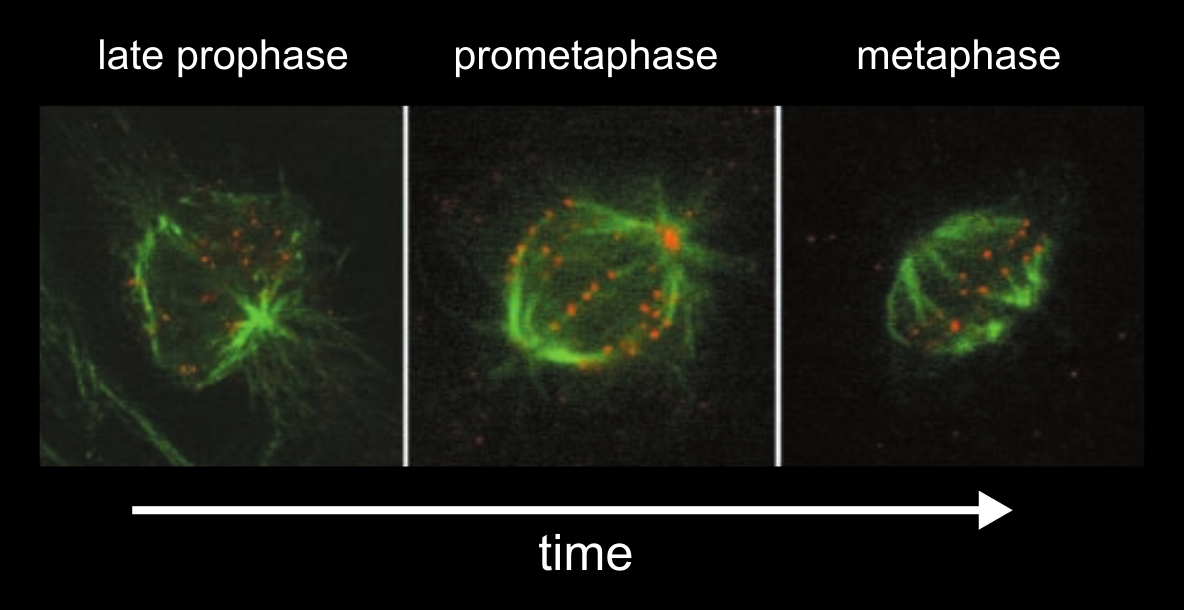
\includegraphics{figures/intro/congression.png}
\caption[Cellule humaine de la prophase à la métaphase]{\label{fig:congression}Cellule
humaine (RPE1) en début de mitose. Les kinétochores (en rouge) sont
alignés à la fin du processus durant la métaphase. On peut deviner les
deux pôles du fuseau en suivant où les microtubules (en vert)
convergent. (DeLuca et al., \hyperref[ref-DeLuca2002]{2002})}
\end{figure}

L'un des modèles de congression propose que les kinétochores soient
capables de « détecter » leur position au sein du fuseau afin de biaiser
leurs mouvements en direction du centre du fuseau mitotique durant la
mitose. Ce mécanisme implique des protéines régulatrices de la dynamique
des microtubules telles que la kinésine-13 et la kinésine-8.

Par exemple, il a été montré qu'un chromosome amphitélique non aligné
dans des cellules humaines accumule l'homologue de la kinésine-13,
appelé MCAK, au niveau du kinétochore qui se déplace vers son pôle (on
parle de « \emph{poleward} kinetochore » ou « kinetochore P » en
anglais), ce qui implique une dépolymérisation biaisée du microtubule et
donc un mouvement plus rapide en direction du centre du fuseau mitotique
(Kline-Smith et al., \hyperref[ref-Kline-Smith2004]{2004}), effet que
l'on retrouve aussi lors des oscillations des chromosomes alignés sur la
plaque métaphasique (Jaqaman et al., \hyperref[ref-Jaqaman2010]{2010}).
Une fois que le chromosome est positionné au niveau de la région
équatorienne du fuseau, la kinésine MCAK disparaît et cet événement
s'accompagne d'une réduction de la force appliquée au niveau du
kinétochore P.

Une autre étude montre que dans des cellules humaines, une accumulation
de l'homologue de la kinésine-8 (Kif18A) proportionnelle à la taille du
microtubule, sur le kinétochore opposé au pôle connecté (on parle de «
\emph{anti-poleward} kinetochore » ou « kinetochore AP » en anglais)
contraint l'amplitude des oscillations des chromosomes en augmentant le
changement de direction du mouvement des chromosomes (Stumpff et al.,
\hyperref[ref-Stumpff2012]{2012}). Dans ce cas là, l'accumulation de la
protéine Kif18A sur le kinétochore AP réduit la dynamique du microtubule
(Du et al., \hyperref[ref-Du2010]{2010}; Stumpff et al.,
\hyperref[ref-Stumpff2011a]{2011}).

Cependant, d'autres études montrent aussi que différents facteurs
pourraient établir un gradient de concentration le long du fuseau et
influencer la position et le mouvement des chromosomes. Par exemple il a
été montré qu'un gradient de Plk1 et Ran-GTP pouvait contrôler la
position des chromosomes (Kiyomitsu and Cheeseman,
\hyperref[ref-Kiyomitsu2012]{2012}) et que Aurora A pourrait former un
gradient au niveau des pôles du fuseau (Hochegger et al.,
\hyperref[ref-Hochegger2013]{2013}; Ye et al.,
\hyperref[ref-Ye2015]{2015}). TODO SYLVIE: se referer au petit schéma.
JE COMPRENDS PAS ? QUEL SCHEMA ?

\subsection{Le mouvement des
chromosomes}\label{le-mouvement-des-chromosomes}

Bien que la congression des chromosomes fasse intervenir des mécanismes
variés et différents au cours de l'évolution, on observe à travers tout
ces mécanismes un processus conservé dans l'ensemble des cellules
eucaryotes : le mouvement oscillatoire des chromosomes (Armond et al.,
\hyperref[ref-Armond2015]{2015}; McIntosh,
\hyperref[ref-McIntosh2012]{2012}; Skibbens et al.,
\hyperref[ref-Skibbens1993]{1993}).

Deux mécanismes sont nécessaires pour produire ce mouvement :

\begin{itemize}
\item
  En premier lieu, les kinétochores frères doivent être soumis à une
  force pour se déplacer. Cette force proviendrait majoritairement de
  l'attachement microtubules - kinétochores. Plusieurs modèles proposent
  différents mécanismes capables de générer une force
  (Civelekoglu-Scholey et al.,
  \hyperref[ref-Civelekoglu-Scholey2006]{2006}; Joglekar and DeLuca,
  \hyperref[ref-Joglekar2009]{2009}; McIntosh,
  \hyperref[ref-McIntosh2012]{2012}; Powers et al.,
  \hyperref[ref-Powers2009a]{2009}). Le modèle stipulant que l'énergie
  proviendrait de la dépolymérisation des microtubules et serait
  transmise par une protéine capable de maintenir l'attachement du
  kinetochore avec le microtubule qui dépolymérise (le complexe NDC80 et
  le complexe DAM1 possiblement) représente en fait une version moderne
  d'un modèle théorique établi dans les années 1990, appelé le modèle de
  Hill (Hill, \hyperref[ref-Hill1985]{1985}). Ces différents mécanismes
  sont détaillés en Section~\ref{sec:force-gen}.
\item
  Une fois que le chromosome est mis en mouvement, un mécanisme doit
  pouvoir réguler sa dynamique afin de contraindre ses déplacements de
  va et vient et de favoriser le maintien de son alignement au milieu du
  fuseau mitotique. Ce mécanisme encore mal compris est probablement dû
  à la contribution de plusieurs phénomènes comme l'instabilité
  directionnelle des kinétochores (Skibbens et al.,
  \hyperref[ref-Skibbens1993]{1993}), le « microtubule poleward flux »
  (Mitchison, \hyperref[ref-Mitchison1989]{1989},
  \hyperref[ref-Mitchison1992]{1992}), le stretch dû au mouvement
  relatif des kinétochores frères (Maddox et al.,
  \hyperref[ref-Maddox2003]{2003}; Skibbens et al.,
  \hyperref[ref-Skibbens1993]{1993}, \hyperref[ref-Skibbens1995]{1995}),
  le gradient de concentration de certaines protéines (Gardner et al.,
  \hyperref[ref-Gardner2008a]{2008}; Jaqaman et al.,
  \hyperref[ref-Jaqaman2010]{2010}; Mayr et al.,
  \hyperref[ref-Mayr2007]{2007}; Stumpff et al.,
  \hyperref[ref-Stumpff2008]{2008}; Varga et al.,
  \hyperref[ref-Varga2006]{2006}) ou encore l'instabilité dynamique des
  microtubules (Amaro et al., \hyperref[ref-Amaro2010a]{2010}; Tirnauer
  and Canman, \hyperref[ref-Tirnauer2002]{2002}).
\end{itemize}

L'un des phénomènes encore mal compris malgré son importance capitale
est le mécanisme par lequel les deux kinétochores frères sont capable de
coordonner leurs états P/AP afin de produire un mouvement régulier et
synchronisé d'une paire de chromosomes.

Un modèle standard du changement de direction d'un chromosome, le «
chromosome switch », a été théorisé en 1994 par Rieder et al. (Rieder,
\hyperref[ref-Rieder1994]{1994}) suite à différentes études sur le
mouvement coordonné des kinétochores frères (Skibbens et al.,
\hyperref[ref-Skibbens1993]{1993}) et le rôle capital de la chromatine
centromérique dans la coordination du changement de direction dans le
mouvement des chromosomes (Skibbens et al.,
\hyperref[ref-Skibbens1995]{1995}).

Ce modèle (Figure~\ref{fig:run-switch}) stipule que l'augmentation de la
tension entre les deux kinétochores qui déclenche le changement d'état
du leading kinétochore en P-AP. La diminution de tension déclencherait
en revanche le changement d'état AP-P du second kinétochore (le trailing
kinétochore).

\begin{figure}[htbp]
\centering
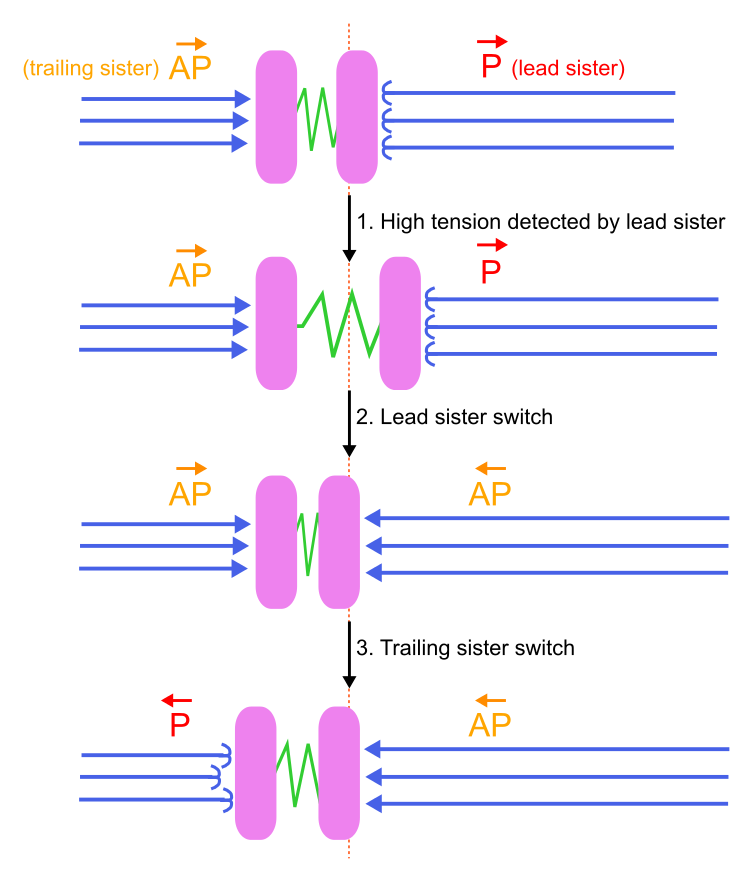
\includegraphics{figures/intro/run_switch.png}
\caption[Modèle standard du changement de direction des kinétochores frères.]{\label{fig:run-switch}Modèle
standard du changement de direction des kinétochores frères. Le leading
kinétochore en se déplaçant plus vite augmente la tension et donc la
distance entre les deux kinétochores. L'augmentation de tension bascule
le leading kinétochore d'un état P à un état AP. Il en résulte une perte
brute de tension et donc de stretch étant donné que les deux
kinétochores se déplacent l'un vers l'autre. Cette relaxation déclenche
alors le changement d'état du trailing kinétochore de AP en P. Les
microtubules en bleu en forme de flèche représentent la polymérisation
tandis que les autres microtubules sont en dépolymérisation.}
\end{figure}

Des observations sur des cellules Ptk1 montrant que le switch est
déclenché lorsque la distance inter-kinétochore est maximum, concorde
avec ce modèle (Wan et al., \hyperref[ref-Wan2012]{2012}). Cependant
beaucoup de questions restent encore ouvertes.

Ce modèle est en accord avec des observations effectuées sur des
cellules Ptk1 qui démontrent que le « switch » est déclenché lorsque la
distance inter-kinétochore est maximum (Wan et al.,
\hyperref[ref-Wan2012]{2012}). Cependant, de nombreuses questions
restent ouvertes

Par exemple certains chromosomes chez les eucaryotes supérieurs
présentent des mouvements très instables sans oscillations apparentes
(Burroughs et al., \hyperref[ref-Burroughs2015]{2015}; Wan et al.,
\hyperref[ref-Wan2012]{2012}). De plus dans les cellules HeLa, dans 30\%
des cas le premier kinétochore qui switch » n'est pas le leading
kinétochore mais le trailing kinétochore (Burroughs et al.,
\hyperref[ref-Burroughs2015]{2015}).

Pour finir, les propriétés du mouvement des chromosomes dans des
cellules eucaryotes comme les levures, qui ne possèdent pas de
chromokinésines sont encore peu connues (Stumpff et al.,
\hyperref[ref-Stumpff2012]{2012}). TODO: IL FAUDRAIT TROUVER UNE PUBLI
AVEC DES TRAJ DE CH CHEZ LA LEVURE AFIN DE DISCUTER DE LA DIFF DES
MOUVEMENTS LEVURE/EUCARYOTE SUP (SINON CEST PAS GRAVE JE NEN PARLERAIS
QUE EN DISCUSSION AVEC MES DONNÉES)

Comment est il alors possible de réconcilier ces différentes
observations avec le modèle standard ?

En 2015, Burroughs et al. ont proposé un nouveau mécanisme qui complète
le modèle standard. Ils partent de l'observation faite que la tension
seule ne pourrait expliquer le déclenchement du changement de direction.
En se basant sur des observations très précises de l'évolution de la
distance inter-kinétochore autour de l'événement de « switch », ils
stipulent qu'une horloge régulerait le taux de catastrophe et de rescue
des microtubules kinétochoriens. Cette régulation influencerait les
forces exercées sur les kinétochores en mouvement et modifierait la
tension entre les deux kinétochores (en accord avec le modèle standard).

Les forces exercées au niveau des kinétochores influencent la dynamique
des chromosomes. Cependant ces forces jouent aussi un rôle structurel au
niveau du fuseau mitotique en contre-balançant les forces générées au
niveau de la zone interdigitée (Courtheoux et al.,
\hyperref[ref-Courtheoux2009]{2009}; Khodjakov et al.,
\hyperref[ref-Khodjakov2004]{2004}) afin de stabiliser la taille du
fuseau durant la métaphase.

\subsection{Le fuseau mitotique : un objet sous
contrainte}\label{le-fuseau-mitotique-un-objet-sous-contrainte}

La métaphase est un moment très particulier de la mitose car c'est le
moment ou le fuseau atteint un état quasi-stationnaire. A ce stade,
l'appareil mitotique subit une contrainte maximum car tous les
chromosomes sont attachés et produisent une force
(Figure~\ref{fig:spindle}). Le complexe cohésine contrebalance les
forces appliquées aux kinétochores. De plus, les microtubules
inter-digitées produisent aussi une force d'extension au niveau du
centre du fuseau. La métaphase est donc le moment où toutes ces forces
s'équilibrent entre elles. Le fuseau est dans un état d'attente qui sera
rompu aussitôt que l'équilibre des forces est brisé par la dégradation
de la cohésine sonnant alors le début de l'anaphase.

Pour donner une idée des forces en jeu, Nicklas a mesuré que la force
maximale que pouvait supporter un chromosome était de l'ordre de 700 pN
(Nicklas, \hyperref[ref-Nicklas1983]{1983}), ce qui correspond à une
force approximative de 10-15 pN par microtubule. Le maintien de la
stabilité mécanique du fuseau métaphasique subissant de telles
contraintes est encore mal compris.

\begin{figure}[htbp]
\centering
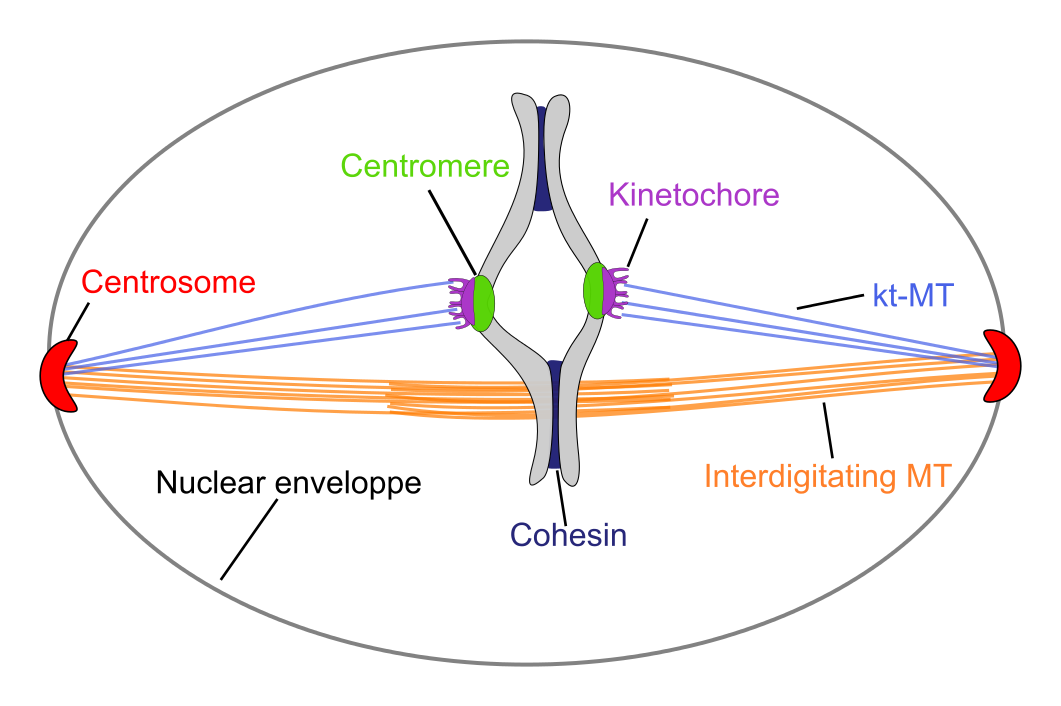
\includegraphics{figures/intro/spindle.png}
\caption[Schéma d'un fuseau mitotique en métaphase]{\label{fig:spindle}Schéma
d'un fuseau mitotique en métaphase (mitose fermé). Les flèches
correspondent aux forces appliquées sur les différents éléments du
fuseau mitotique.}
\end{figure}

\subsection{Le point de contrôle de la transition
métaphase/anaphase}\label{le-point-de-contruxf4le-de-la-transition-muxe9taphaseanaphase}

Le point de contrôle de l'assemblage du fuseau (« Spindle Assembly
Checkpoint » ou SAC en anglais) maintient la stabilité génomique en
retardant la division cellulaire jusqu'à ce que la fidélité de tous les
attachements soit garantis (voir Lara-Gonzalez et al.
(\hyperref[ref-Lara-Gonzalez2012]{2012}) pour une revue). Quand un
attachement est incorrect (Figure~\ref{fig:attachements}), il y a
activation du SAC et blocage du cycle cellulaire.

Jusqu'à la métaphase les chromatides sœurs sont maintenues entre elles
par un complexe protéique appelé la cohésine (Nasmyth and Haering,
\hyperref[ref-Nasmyth2009]{2009}). L'entrée en anaphase active un
mécanisme de dégradation de la cohésine. Une fois le lien entre les
chromatides sœurs disparu, chacune des chromatides va migrer en
direction du pôle vers lequel elle est attachée, c'est l'anaphase.

Lorsque tous les kinétochores sont attachés de manière stable, alors le
SAC se désactive et une cascade métabolique dégrade le complexe cohésine
(Figure~\ref{fig:sac}).

Les kinétochores non-attachés génèrent un signal « ON » à l'attention du
SAC en recrutant un complexe protéique composé principalement de 4
protéines Mad2, BubR1, Bub3 et Cdc20 (Sudakin et al.,
\hyperref[ref-Sudakin2001]{2001}) appelé le « Mitotic Checkpoint Complex
» (MCC) (Figure~\ref{fig:sac}). Ce complexe, à ce jour connu pour être
l'inhibiteur principal de l'APC/C, est une E3 ubiquitine ligase qui
cible des protéines du cycle cellulaire afin de les dégrader par
protéolyse (Pines, \hyperref[ref-Pines2011]{2011}). L'une des cibles de
l'APC/C est la sécurine qui inhibe la protéine capable de cliver la
cohésine appelée la séparase (Figure~\ref{fig:sac}).

\begin{figure}[htbp]
\centering
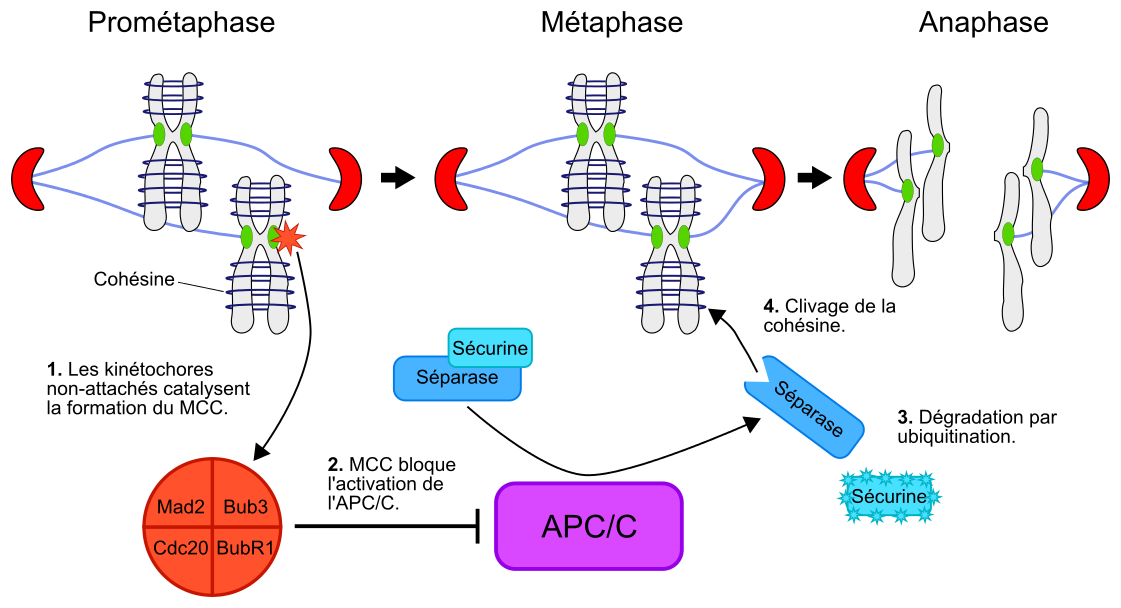
\includegraphics{figures/intro/sac.png}
\caption[Le mécanisme d'action du SAC]{\label{fig:sac}Le mécanisme
d'action du SAC. Les chromosomes non-attachés catalysent la formation du
MCC au niveau du kinétochore. Le MCC bloque l'activité de l'ubiquitine
ligase APC/C. Une fois tous les kinétochores correctement attachés,
l'APC/C dégrade la sécurine, ce qui active la séparase qui clive le
complexe protéique de la cohésine.}
\end{figure}

La façon dont les kinétochores non-attachés recrutent le MCC implique un
réseau complexe de protéines situées au niveau du kinétochore. Pour une
revue détaillée voir Musacchio and Salmon
(\hyperref[ref-Musacchio2007]{2007}).

Le réseau métabolique, dont fait partie le SAC, peut être modélisé comme
une cascade de réactions chimiques (voir Novak and Tyson
(\hyperref[ref-Novak1995]{1995}) pour un exemple de modélisation chez la
levure à fission). Ce type de problème dynamique est souvent modélisé à
l'aide d'un système d'équations différentielles. Bien que les modèles de
réseaux métaboliques puissent prendre en compte la dimension spatiale
des processus étudiés en compartimentant les réactions, il manque la
prise en compte d'une réelle géométrie de la cellule ou des objets la
composant.

\section{Modélisation mathématique de la
mitose}\label{moduxe9lisation-mathuxe9matique-de-la-mitose}

La mitose est un processus qui fascine depuis longtemps les biologistes
mais aussi les scientifiques en dehors des sciences du vivant. Les
physiciens s'intéressent aux propriétés mécaniques du fuseau mitotique
ainsi qu'aux forces mises en jeu durant ce processus. Tandis que les
mathématiciens sont plus concernés par le développement d'un modèle
mathématique universel qui pourrait décrire la mitose.

\subsection{Que signifie « modéliser un processus biologique »
?}\label{que-signifie-moduxe9liser-un-processus-biologique}

La modélisation est un vaste champ de recherche et il existe une grande
variété de classes de modèle. Les expériences de modélisation effectuées
durant ce travail et d'une manière plus générale, les modèles
mathématiques utilisés en biologie cellulaire pour décrire la mitose
sont « des modèles de connaissance ». C'est à dire qu'ils sont tous
construits à partir d'une analyse physique, biologique et chimique des
connaissances existantes sur la mitose.

Un modèle de connaissance est bâti à la fois sur un ensemble de lois
générales (mécanique, électromagnétisme, thermodynamique, etc.) ainsi
que sur un ensemble de lois empiriques qui gouvernent les différents
phénomènes du processus étudié.

C'est la classe de modèle par excellence car les équations le composant
décrivent directement les processus en jeu. Cependant certains
phénomènes très complexes ne peuvent pas toujours être modélisés par
cette approche. On utilise donc parfois une autre classes de modèle
(comme les modèles de « boites noires », non discutés ici). On notera
qu'il est aussi possible d'appliquer une série d'approximations afin de
réduire la complexité du processus étudié et ainsi d'utiliser un modèle
de connaissance, au prix d'une précision moins importante.

Avant de continuer, il est important de répondre à une question
primordiale qui revient souvent chez les biologistes : pourquoi
modélise-t-on ?

Un scientifique tire des conclusions en fonction des différents
résultats produits par ses expériences. Une déduction logique lui permet
donc de bâtir un « modèle » qualitatif du processus qu'il étudie. Ce
modèle est parfois représenté sous la forme d'un schéma à la fin d'un
article ou d'une présentation.

Un modèle mathématique est la version quantitative de ce modèle-schéma
décrivant un processus biologique (Figure~\ref{fig:modelling}).

\begin{figure}[htbp]
\centering
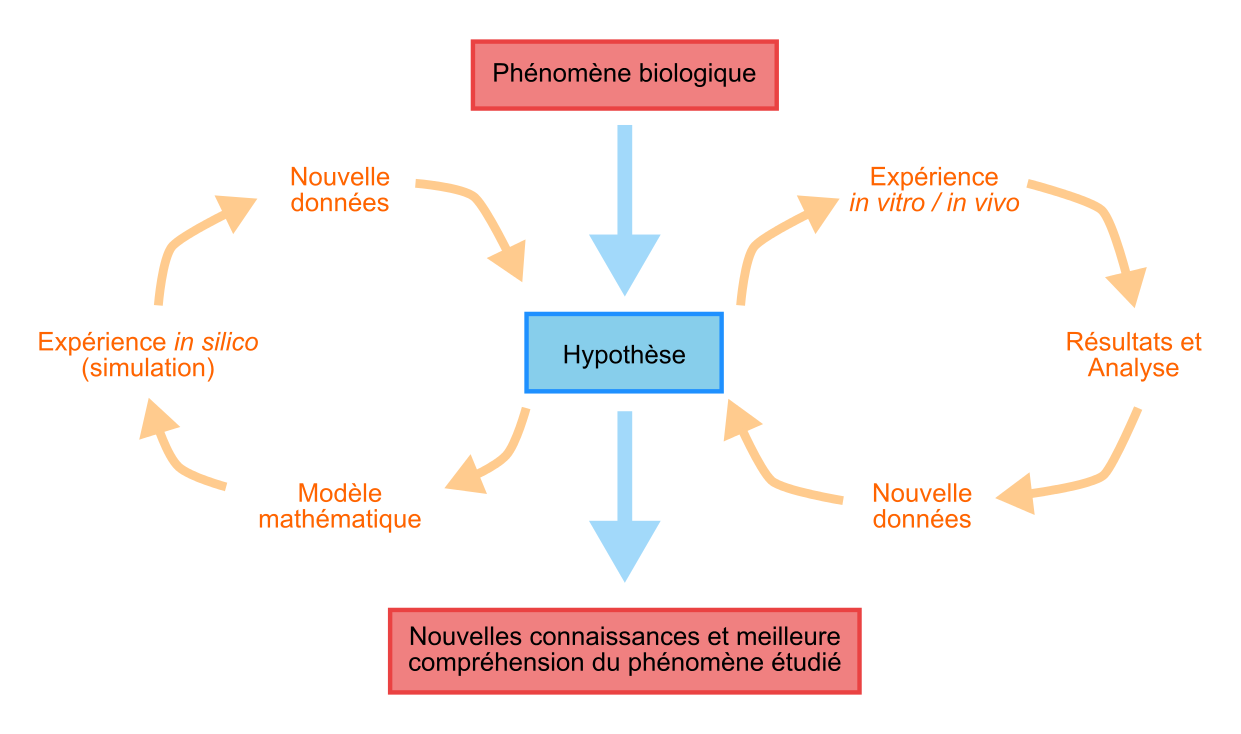
\includegraphics{figures/intro/modelling.png}
\caption[Workflow de l'approche modélisation en biologie]{\label{fig:modelling}Schéma
reproduisant un workflow expérimental possible lors de l'étude d'un
phénomène biologique par une approche de modélisation (adapté de Woelke
et al. (\hyperref[ref-Woelke2010]{2010})).}
\end{figure}

Il peut apporter une vision plus précise du processus étudié, notamment
en quantifiant différents paramètres et propriétés du système qui
peuvent par la suite être comparés à des mesurables décrivant le
processus \emph{in vivo}.

La modélisation mathématique a pris son essor avec la modernisation des
ordinateurs et du calcul numérique durant ces 20 dernières années. Cet
outil, parfois complexe à appréhender et à comprendre, est la continuité
naturelle des modèles mentaux que les scientifiques établissent par la
déduction logique depuis toujours.

La mitose est un processus cellulaire d'une extrême complexité en grande
partie due au grand nombre de phénomènes mis en jeu dans un volume si
petit. Il en résulte qu'il est à ce jour, en 2015, encore hors de notre
portée de modéliser avec précision la mitose dans son intégralité.
Chaque modèle s'applique donc à décrire un moment bien spécifique de la
mitose avec un niveau de précision plus ou moins important. Ces deux
variables expliquent la grande diversité des modèles existants.

Pour finir on soulignera l'existence de nombreux modèles décrivant des
phénomènes biologiques très spécifiques tels que l'instabilité dynamique
des microtubules (Bowne-Anderson et al.,
\hyperref[ref-Bowne-Anderson2013]{2013}; Nedelec and Foethke,
\hyperref[ref-Nedelec2007]{2007}), la génération de force au niveau de
l'attachement kinétochore-microtubule (Keener and Shtylla,
\hyperref[ref-Keener2014]{2014}, Shtylla and Keener,
\hyperref[ref-Shtylla2011]{2011}), l'effet de certaines kinésines sur la
dynamique des microtubules (Hough et al.,
\hyperref[ref-Hough2009]{2009}; Reese et al.,
\hyperref[ref-Reese2014]{2014}). Ces modèles sortent du cadre d'une
description générale du processus de la mitose et ne seront pas discutés
ici.

\subsection{Comment modéliser le mouvement des chromosomes
?}\label{comment-moduxe9liser-le-mouvement-des-chromosomes}

Tout système mécanique peut se modéliser en résolvant les équations des
forces appliquées sur le système. Cette approche a été utilisée pour la
première fois par Scholey et al. afin de modéliser le mouvement des
chromosomes durant la mitose (Civelekoglu-Scholey et al.,
\hyperref[ref-Civelekoglu-Scholey2006]{2006}). Par la suite, l'équipe de
Tournier et al. a repris l'idée original du modèle de « force balance »
afin d'étudier la ségrégation des chromosomes en supposant des
attachements stochastiques entre les microtubules et les kinétochores
(Gay et al., \hyperref[ref-Gay2012a]{2012}).

Le cadre théorique sur lequel est basé ce travail est une adaptation du
modèle de Tournier et al.. Les deux sections suivantes détaillent
l'approche physique utilisée dans ce modèle.

\subsubsection{Types de forces en jeux}\label{types-de-forces-en-jeux}

Une force est une « influence » qui peut provoquer l'accélération d'une
particule ou la déformation d'un objet contraint (Howard,
\hyperref[ref-Howard2001]{2001}). Les forces peuvent avoir pour origines
des processus physiques très divers. En voici une liste non exhaustive :

\begin{itemize}
\item
  les forces \textbf{magnétiques}, d'amplitude très faible au niveau
  moléculaire, sont provoquées par un champs magnétique qui s'applique
  sur des protons possédant un moment magnétique.
\item
  un objet de masse \(m\) subit une force \textbf{gravitationnelle} de
  magnitude \(mg\), où \(g\) est l'accélération causée par la gravité.
  Au niveau cellulaire cette force est très petite.
\item
  une force \textbf{centrifuge} est subi par un objet en rotation. Sa
  magnitude vaut \(ma_c\), où \(a_c\) correspond à l'accélération
  centrifuge. On peut aussi noter que la force centripète est la force
  opposée à la force centrifuge qui empêche un objet en rotation de «
  fuir » le centre.
\item
  une force \textbf{optique} est une force de collision correspondant à
  une pression optique dû au moment cinétique des photons. Les photons
  peuvent donc exercer une force quand ils sont diffractés par un objet.
  Cette force est très faible dans la nature, par exemple si une
  molécule absorbe \(10^9\) photons par seconde (cela correspond à un
  laser puissant), la force optique ne sera que de \(10^{-6}pN\).
\item
  les forces \textbf{thermiques} sont un autre type de force de
  collision dues au choc sur un objet par une multitude d'objets de
  taille plus faible. Par exemple une protéine en suspension dans de
  l'eau va subir une force thermique à cause du choc des molécules d'eau
  à sa surface. L'ensemble des collisions provenant de toutes les
  directions, il en résulte une force totale net aléatoire. La force
  appliquée sur une protéine de \(100kDa\) est de l'ordre de \(500pN\).
  Cette force gouverne un processus physique appelé mouvement brownien
  ou encore marche aléatoire.
\item
  les forces \textbf{électrostatiques} s'appliquent à une particule
  chargé \(q\) par un champ éléctrique \(E\). Elle est de magnitude
  \(F = qE\). Ces forces sont à l'origine du lien qui attache les
  différents atomes d'une molécule.
\end{itemize}

La nature très diverse de ces forces ainsi que la difficulté à les
mesurer à des échelles microscopiques les rend difficilement utilisables
pour l'étude des processus cellulaires et subcellulaires.

Afin d'étudier des systèmes mécaniques à des échelles cellulaires et
subcellulaires on utilise trois éléments mécaniques fondamentaux qui
sont le ressort, l'amortisseur et la masse. En effet, une protéine ou un
élément subcellulaire peut être assimilé à un système mécanique composé
d'atomes qui ont une masse, reliés par des liens qui possèdent une
élasticité.

D'après la seconde loi de Newton, la masse provoque une accélération
constante égale à \(a = F/m\) où \(a\) est l'accélération, \(F\) la
force appliqué et \(m\) la masse (Figure~\ref{fig:force_types}). Si on
définit l'accélération \(a\) comme étant la dérivée première de la
vitesse \(v\) et la dérivée seconde de la position \(x\) par rapport au
temps \(t\), on a :

\[
F = ma = m\frac{dv}{dt} = m\frac{dx^2}{dt^2}
\]

Un amortisseur est un élément mécanique qui répond à une force appliquée
en se déformant à vitesse constante avec une magnitude de
\(v = F/\gamma\), où γ correspond au coefficient de viscosité
(Figure~\ref{fig:force_types}). Cet objet idéal est utilisé pour
modéliser le mouvement d'un objet dans un fluide comme par exemple une
cuillère qu'on insère dans un pot de miel. L'action de tirer rapidement
la cuillère hors du pot, peut soulever le pot à cause du coefficient de
viscosité élevé du miel qui va contrer la force de la cuillère tirée de
manière proportionnelle à la vitesse.

Enfin, un élastique est un élément mécanique qui s'allonge en réponse à
une force. L'allongement d'un élastique par rapport à sa longueur de
repos est égale à \(L = F/\kappa\), où \(\kappa\) la constante
d'élasticité et \(L\) l'allongement (Figure~\ref{fig:force_types}). Si
la constante d'élasticité est indépendante de la force ou de
l'extension, on dit que l'élastique suit la loi de Hooke.

\begin{figure}[htbp]
\centering
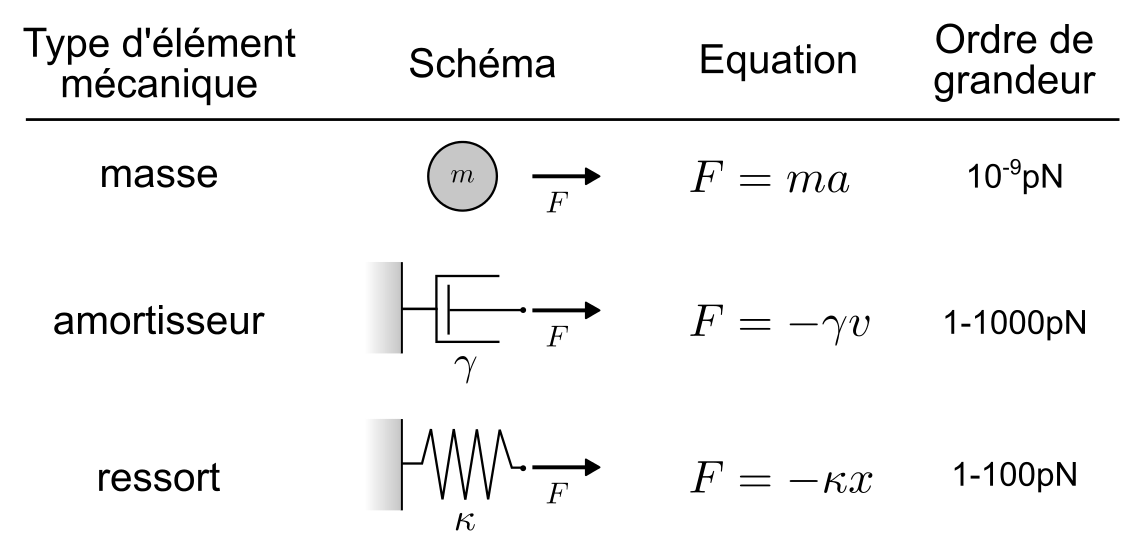
\includegraphics{figures/intro/force_types.png}
\caption[Schéma des trois éléments mécaniques fondamentaux]{\label{fig:force_types}Schéma
des trois éléments mécaniques fondamentaux : la masse, l'amortisseur et
le ressort (adapté de Howard (\hyperref[ref-Howard2001]{2001})). Les
ordres de grandeurs correspondent à la magnitude des forces rencontrées
au niveau moléculaire : forces élastiques pour le ressort, forces
visqueuses pour l'amortisseur et force gravitationnelles pour la masse.}
\end{figure}

Ces trois éléments mécaniques sont donc suffisant pour modéliser avec
une bonne approximation un grand nombre de systèmes mécaniques complexes
comme par exemple le fuseau mitotique. Pour cela on construit une
géométrie en assemblant ces différents éléments en série ou en parallèle
les uns par rapport aux autres. Puis on utilise l'équation du mouvement
afin de calculer la dynamique du système.

\subsubsection{L'équation du mouvement}\label{luxe9quation-du-mouvement}

Une fois le système mécanique décrit, on utilise l'équation du mouvement
afin de suivre l'évolution de la position de chaque objet du système
dans le temps, défini par :

\[
F = m\frac{dx^2}{dt^2} + \gamma\frac{dx}{dt} + \kappa x
\]

Où le premier terme inertiel est la seconde loi de Newton, le second
terme correspond aux forces visqueuses et le troisième terme est du aux
forces élastiques. \(F\) correspond à toutes les autres forces externes
appliquées au système (Figure~\ref{fig:motion_equation}).

\begin{figure}[htbp]
\centering
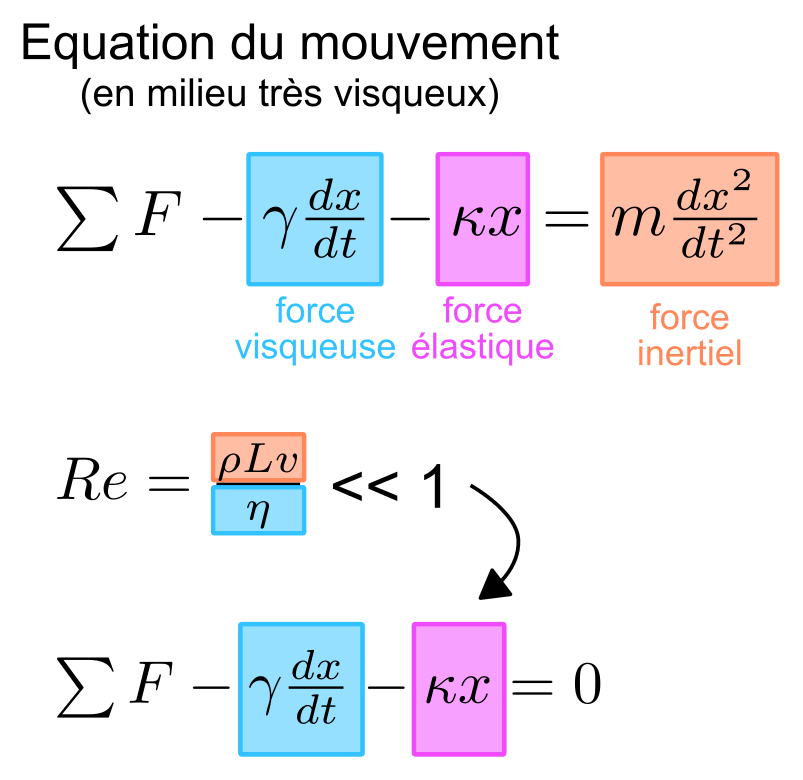
\includegraphics{figures/intro/motion_equation.png}
\caption[L'équation du mouvement]{\label{fig:motion_equation}L'équation
du mouvement décrit l'évolution spatial d'un objet au cours du temps
sous l'action de plusieurs forces qui lui sont appliquées. Le terme
inertiel peut être omis dans le cas d'un objet évoluant dans un système
très visqueux pour des nombres de Reynolds très bas.}
\end{figure}

Le terme inertiel étant une dérivée seconde de la position par rapport
au temps \(\frac{dx^2}{dt^2}\), sa résolution numérique ou algébrique
peut être complexe et rendre les temps de calcul relativement long
(C'EST BIEN DE METTRE CA???).

Il est possible d'approximer l'équation du mouvement en enlevant le
terme inertiel lorsqu'on étudie des systèmes où la force inertielle est
négligeable par rapport aux forces visqueuses. Par exemple dans le cas
d'un système évoluant dans un milieu très visqueux par rapport à sa
masse comme dans une cellule. Ce rapport entre les deux forces est
symbolisé par le nombre de Reynolds.

\[
Re = \frac{\rho Lv}{\eta}
\]

Où \(\rho\) est la densité du fluide, \(L\) la longueur caractéristique
de l'objet, \(v\) sa vitesse et \(\eta\) sa viscosité. Quand
\(Re << 1\), cela signifie que les forces dues à la masse sont
négligeables par rapport aux forces visqueuses, ce qui est le cas dans
un système subcellulaire (Figure~\ref{fig:motion_equation}).

On peut donc approximer l'équation du mouvement comme suit :

\[
F = \gamma\frac{dx}{dt} + \kappa x
\]

\subsubsection{Application au fuseau
mitotique}\label{application-au-fuseau-mitotique}

Dans le cas du fuseau mitotique, on identifie en premier lieu,
l'ensemble des différents objets qui composent le fuseau tel que les
pôles, les kinétochores, les sites d'attachement, etc. Ensuite on
définit les propriétés visco-élastiques décrivant chacun des objets pour
ensuite définir les forces appliquées sur le système. Par exemple la
force due à un attachement élastique entre les deux kinétochores (qui
correspond à la cohésine) va dépendre de la position relative des deux
kinétochores l'un par rapport à l'autre et du paramètre de raideur
\(\kappa\) qui caractérise la cohésine et qui peut être déterminé
\emph{in vivo} (Figure~\ref{fig:spindle_model}).

\begin{figure}[htbp]
\centering
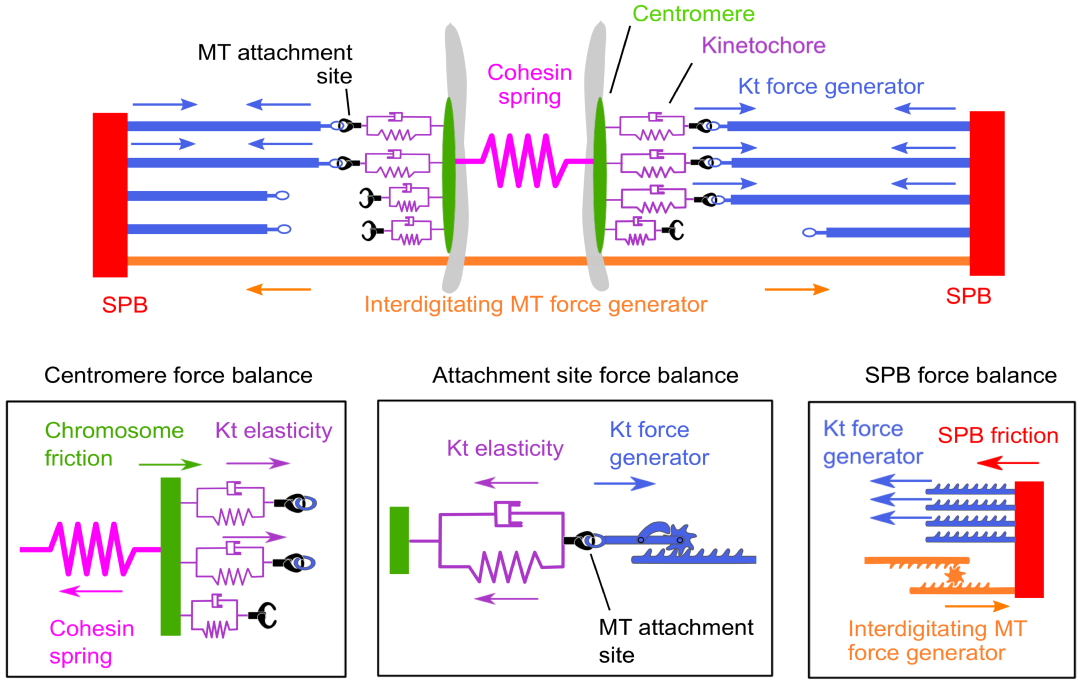
\includegraphics{figures/intro/spindle_model.png}
\caption[Modélisation mécanique du fuseau mitotique]{\label{fig:spindle_model}Le
fuseau modélisé est composé de différents objets ayant des propriétés
visco-élastique définies. On décrit aussi les forces appliquées sur les
objets comme par exemple la force motrice qui tire sur un site
d'attachement (en violet) quand un microtubule s'y attache (en bleu)
(Gay et al., \hyperref[ref-Gay2012a]{2012})}
\end{figure}

Dans un système mécanique tel que celui-là, il est difficile de prédire
la réponse du système aux forces appliquées. On assume donc qu'en chaque
point de l'espace la somme des forces appliquées au système est nulle :

\[
F - \gamma\frac{dx}{dt} - \kappa x = 0
\]

Cette équation différentielle peut ensuite être résolue afin de
déterminer la vitesse et donc la position de chaque objet dans le temps.

On peut alors construire un système d'équation linéaire décrivant le
système mécanique du fuseau mitotique (voir Gay et al.
(\hyperref[ref-Gay2012a]{2012}) pour le système d'équation complet). La
résolution numérique permet alors d'accéder aux trajectoires des
kinétochores et des pôles (Figure~\ref{fig:traj_model}).

\begin{figure}[htbp]
\centering
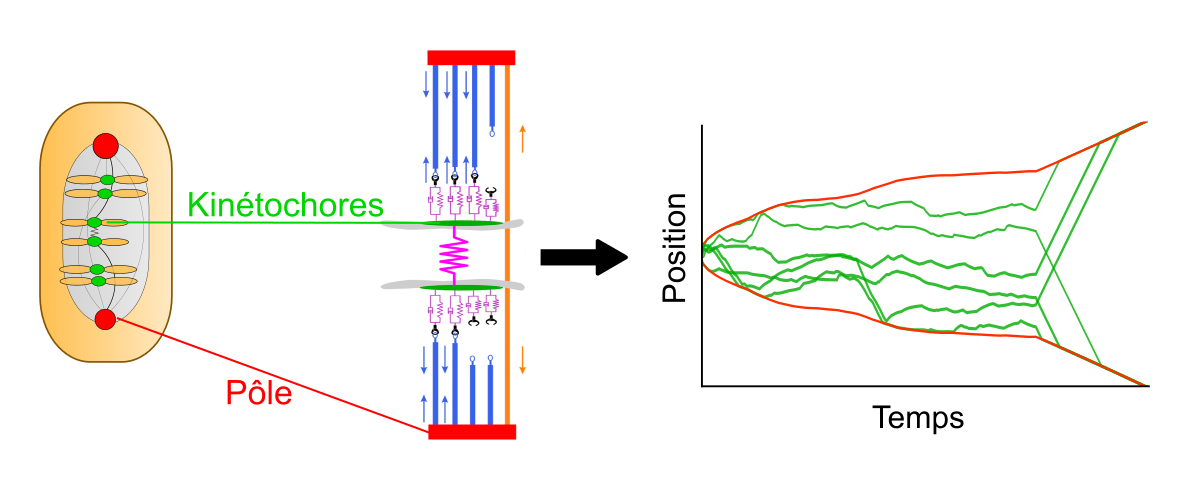
\includegraphics{figures/intro/traj_model.png}
\caption[Trajectoire des chromosomes \_in silico\_]{\label{fig:traj_model}Une
simulation numérique permet de résoudre l'équation du mouvement et
ensuite accéder à l'évolution des positions de chaque objet au cours du
temps.}
\end{figure}

\subsection{L'assemblage du fuseau
mitotique}\label{lassemblage-du-fuseau-mitotique}

Durant l'assemblage du fuseau mitotique, le fuseau en cours de
formation, « capture » les chromosomes par l'intermédiaire des
microtubules. Ce processus de capture est étudié et modélisé depuis
longtemps, ce qui en fait un bon exemple d'utilisation de la
modélisation mathématique dans l'étude d'un processus biologique.

Le modèle le plus répandu décrivant l'assemblage du fuseau mitotique est
celui appelé « recherche et capture » (Figure~\ref{fig:mogilner}).
Durant la prométaphase, les microtubules s'assemblent aux deux pôles du
fuseau et vont « sonder » l'espace de manière stochastique afin
d'attacher chacun des kinétochores. Des simulations numériques ont
montré que ce processus seul n'est pas assez efficace pour expliquer les
temps de prométaphase, rencontrés dans la plupart des organismes de
l'ordre d'une dizaine de minutes (Wollman et al.,
\hyperref[ref-Wollman2005]{2005}). Il existe donc des biais durant ce
processus permettant une capture plus rapide et fidèle des chromosomes.

\begin{figure}[htbp]
\centering
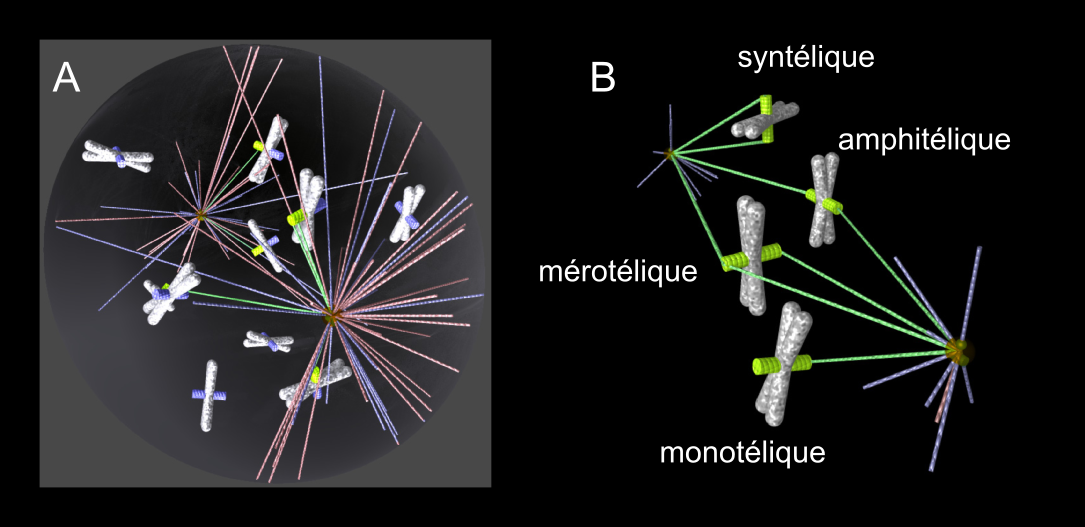
\includegraphics{figures/intro/mogilner.png}
\caption[Modèle numérique de l'assemblage du fuseau]{\label{fig:mogilner}Modèle
numérique de l'assemblage du fuseau (Paul et al.,
\hyperref[ref-Paul2009]{2009}). \textbf{A}. Des chromosomes durant la
phase « recherche et capture ». Certains kinétochores sont attachés (en
vert) et d'autres sont non attachés (en bleu). \textbf{B}. 4 types
d'attachements possibles des chromosomes.}
\end{figure}

Un modèle propose que l'un de ces biais puisse être la présence d'un
gradient de RanGTP autour des kinétochores
(Figure~\ref{fig:assembly_time}). Une plus forte concentration de RanGTP
stabiliserait les microtubules et les feraient croître en direction des
kinétochores (loin des pôles). Des simulations numériques ont montré que
ce biais spatial lors du processus de recherche augmenterait la vitesse
de capture (Wollman et al., \hyperref[ref-Wollman2005]{2005}).

\begin{figure}[htbp]
\centering
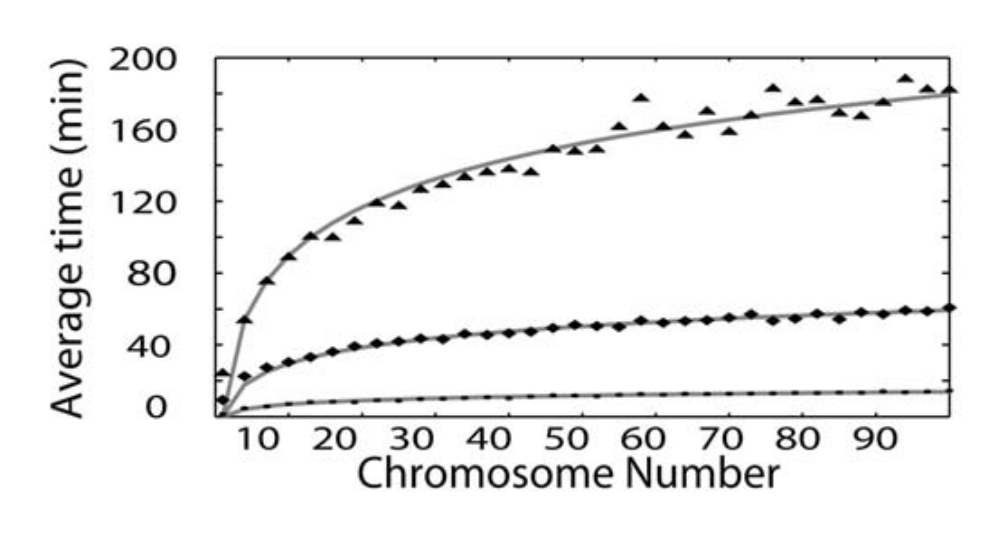
\includegraphics{figures/intro/assembly_time.png}
\caption[Temps moyen de capture des chromosomes]{\label{fig:assembly_time}Temps
moyen de capture de tous les chromosomes en fonction du nombre de
chromosomes total pour trois modèles différents \emph{in silico} :
modèle non-biaisé (recherche aléatoire) avec 1000 MTs (triangles),
modèle biaisé (gradient de RanGTP) avec 250 MTs (losanges), modèle
biaisé avec 1000 MTs (cercles) (Wollman et al.,
\hyperref[ref-Wollman2005]{2005}).}
\end{figure}

Cependant ce modèle encore trop naïf n'explique pas la précision avec
laquelle le fuseau attache les chromosomes, en évitant les attachements
syntéliques et mérotéliques. En effet des simulations de « recherche et
capture » aléatoires ont montré la présence de 65\% d'attachements
mérotéliques et seulement 15\% d'attachements amphitéliques (Paul et
al., \hyperref[ref-Paul2009]{2009}).

Deux mécanismes pourraient expliquer la précision des attachements
\emph{in vivo}. Le premier stipule que lors d'un attachement
monotélique, le chromosome effectue une rotation de telle façon que le
kinétochore attaché se positionne face à son pôle tandis que son
kinétochore frère ferait face au pôle opposé et aurait donc une plus
forte probabilité de s'y attacher (Figure~\ref{fig:spindle_assembly}A).
Ce mécanisme réduit de manière importante le pourcentage d'erreurs quand
il est inclus dans des simulations numériques (Mogilner and Craig,
\hyperref[ref-Mogilner2010]{2010}; Paul et al.,
\hyperref[ref-Paul2009]{2009}).

Le second mécanisme serait que l'attachement amphitélique apparaît de
manière évolutive (un peu à la façon d'un processus Darwinien). C'est à
dire que la capture serait un processus d'essais et d'erreurs itératif.
Au début, les attachements syntéliques sont fréquents et disparaissent
souvent (Lampson et al., \hyperref[ref-Lampson2004]{2004}) jusqu'à ce
que seuls les attachements amphitéliques soient conservés. Ceci est
possible seulement si les taux d'attachement et de détachement dépendent
de l'état d'attachement du kinétochore comme illustré
Figure~\ref{fig:spindle_assembly}B. Ici aussi des simulations numériques
ont montré que ce mécanisme réduit de manière très importante le nombre
d'erreurs d'attachement (Mogilner and Craig,
\hyperref[ref-Mogilner2010]{2010}; Paul et al.,
\hyperref[ref-Paul2009]{2009}).

Le mécanisme modulant les probabilités d'attachement en fonction de
l'état du kinétochore pourrait impliquer une protéine telle que Aurora B
comme déjà discuté en Section~\ref{sec:attachments-type}.

\begin{figure}[htbp]
\centering
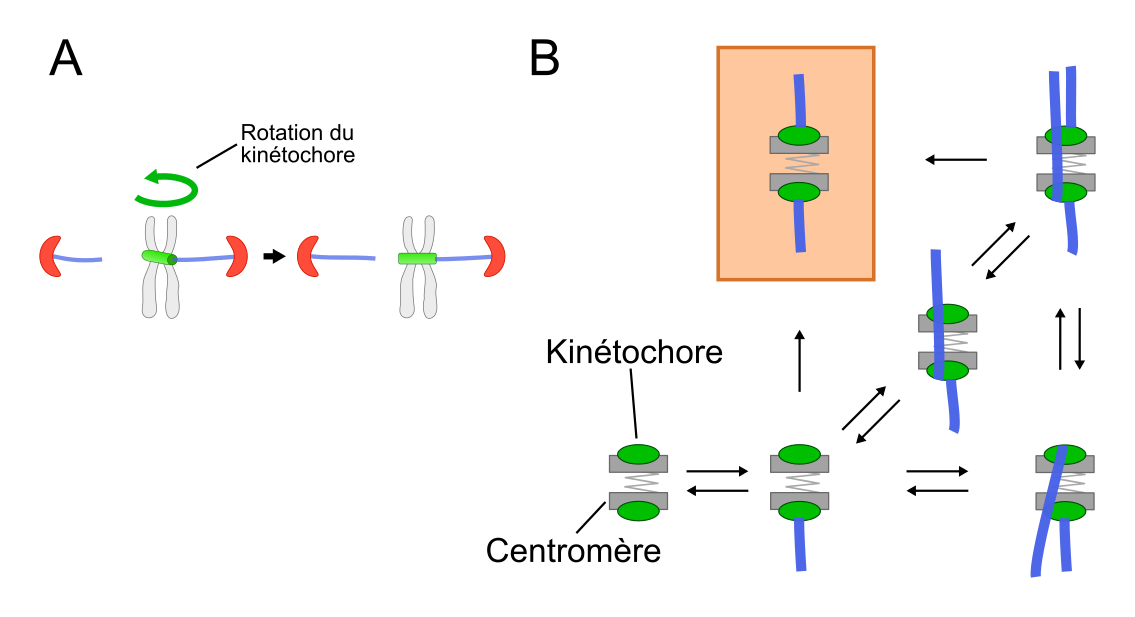
\includegraphics{figures/intro/spindle_assembly.png}
\caption[Deux mécanismes de l'assemblage du fuseau mitotique]{\label{fig:spindle_assembly}Deux
mécanismes expliquant la fidélité des attachements durant le processus
de « recherche et capture ». \textbf{A}. Mécanisme impliquant
l'orientation du kinétochore frère en réponse à un attachement
monotélique. \textbf{B}. Mécanisme évolutif qui « sélectionne »
l'attachement amphitélique (box couleur saumon) avec le temps en
explorant différents états d'attachement.}
\end{figure}

\subsection{La dynamique des
chromosomes}\label{la-dynamique-des-chromosomes}

\label{sec:force-gen}

La trajectoire des chromosomes en métaphase peut être reconstruite
\emph{in vivo} de manière très précise (Armond et al.,
\hyperref[ref-Armond2015]{2015}; Jaqaman et al.,
\hyperref[ref-Jaqaman2010]{2010}; Ke et al.,
\hyperref[ref-Ke2009]{2009}; Wan et al., \hyperref[ref-Wan2012]{2012}),
ce qui permet de comprendre les propriétés à la fois biochimiques et
biophysiques gouvernant le mouvement, la position et l'attachement des
chromosomes. Cependant les techniques d'acquisition par microscopie à
fluorescence ne permettent pas pour le moment de résoudre l'état
d'attachement ainsi que d'accéder aux différentes forces mise en jeu
durant ce phénomène. La modélisation mathématique peut être une façon
d'accéder à ces propriétés pour peu que le modèle en question puisse
reproduire avec fidélité la trajectoire des chromosomes \emph{in vivo}.

L'un des phénomènes qui reste encore largement mystérieux dans le
mouvement des chromosomes durant la mitose est le mécanisme qui permet
au kinétochore de maintenir son attachement à des microtubules qui
dépolymérisent. L'un des premiers modèles expliquant ce phénomène est le
modèle de Hill (Hill, \hyperref[ref-Hill1985]{1985}). Ce modèle (« Hill
sleeve model » en anglais) utilise des propriétés classiques de
cinétique et thermodynamique pour montrer comment un microtubule qui
dépolymérise peut rester attaché profondément dans une région du
kinétochore composée de « crans » qui sont autant de mini barrières
d'énergie (Figure~\ref{fig:hill_model}A). Les hétérodimères de tubuline
interagissent avec un nombre fini de sites d'attachements le long de
cette région du kinétochore avec une affinité modérée. L'insertion est
donc contrôlée par les fluctuations thermiques et le microtubule peut
perdre des sous-unités (dépolymérisation) aux endroits accessibles,
c'est à dire dans la région la plus profonde du kinétochore. Le
mouvement du microtubule est donc contraint et biaisé par différentes
barrières d'énergie dues aux nombreux attachements du microtubule dans
cette région du kinétochore.

Au début des années 2000, un modèle fondé sur l'idée du modèle de Hill
et incluant une balance de force des différents composants du fuseau
mitotique est proposé. Les auteurs ont généralisé le précédent modèle en
prenant en compte les deux chromatides sœurs ainsi que plusieurs sites
d'attachements par kinétochore (Joglekar and Hunt,
\hyperref[ref-Joglekar2002]{2002}). Les sites d'attachements de chaque
microtubule sont insérés au niveau de la plaque externe du kinétochore
et sont modélisés comme un ressort suivant la loi de Hook (« Hookean
spring » en anglais). Les forces de tensions entre les kinétochores
frères dues à la cohésine sont aussi prises en compte.

Ces deux modèles supposent donc que le principal acteur qui dirige le
mouvement des chromosomes est la dynamique des microtubules. Le modèle
de Hill est un modèle théorique car les protéines composant la région «
crantée » du kinétochore ne sont pas spécifiées.

\begin{figure}[htbp]
\centering
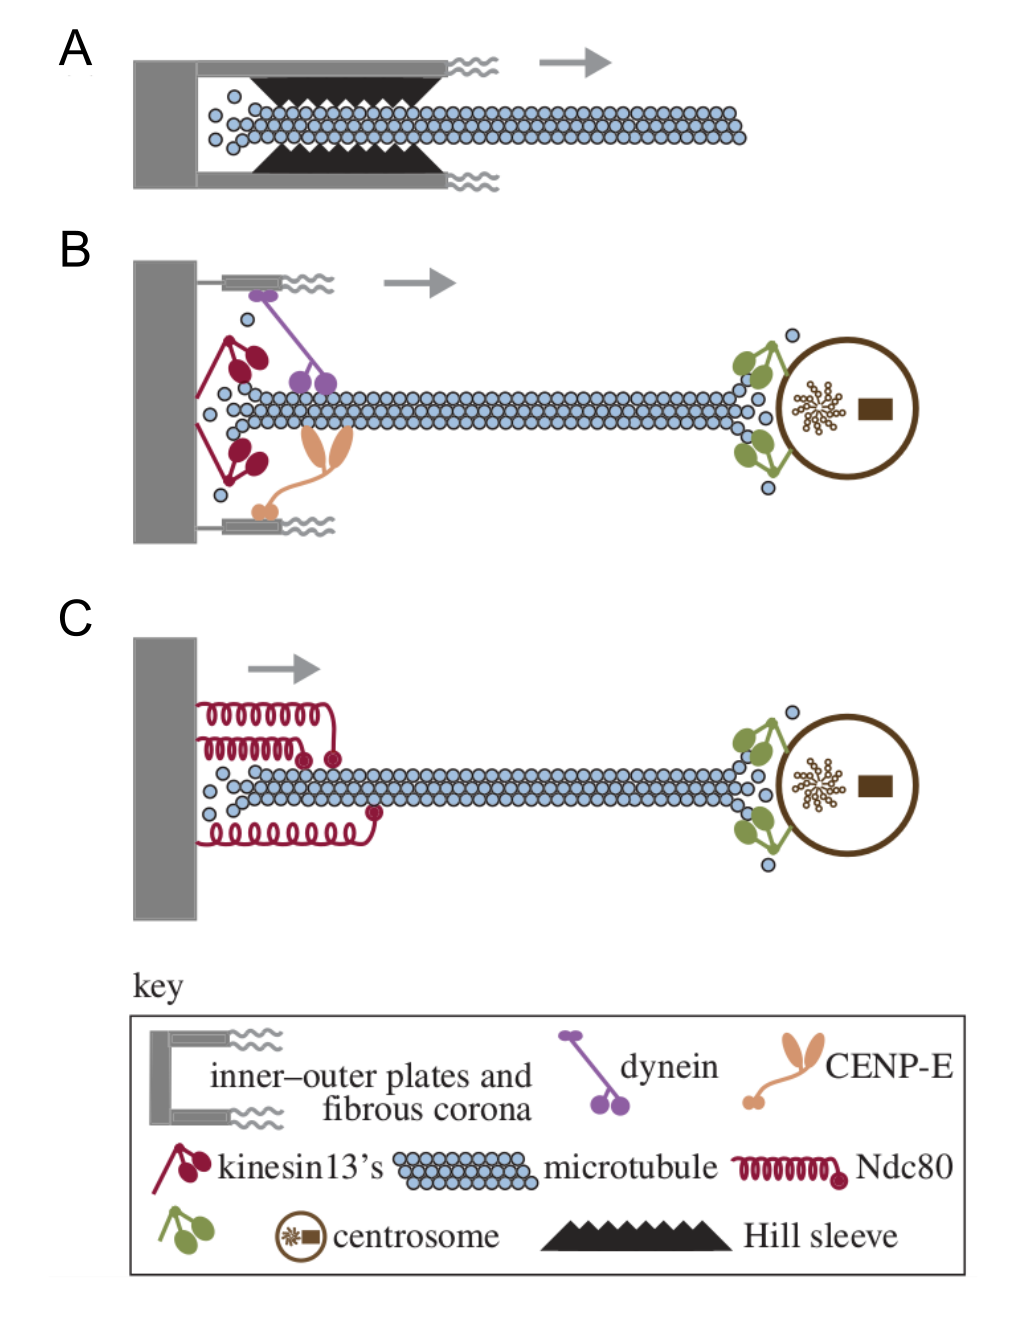
\includegraphics{figures/intro/hill_model.png}
\caption[Différents modèles de types d'attachement entre le microtubule et le kinétochore]{\label{fig:hill_model}Différents
modèles de types d'attachement entre le microtubule et le kinétochore
(Civelekoglu-Scholey and Cimini,
\hyperref[ref-Civelekoglu-Scholey2014]{2014}). \textbf{A}. « Hill sleeve
model » qui suppose l'existence d'un nombre fini de sites d'attachements
arrangés en série. \textbf{B}. Une balance de force est mise en place
entre différentes protéines motrices localisées aux pôles du fuseau et
au kinétochore. \textbf{C}. L'attachement se fait par un complexe
protéique non moteur appelé NDC80. Il fait office de coupleur
dynamique.}
\end{figure}

En 2006, une autre équipe proposa un modèle alternatif en se référant à
des observations faites \emph{in vivo} montrant que des protéines
motrices étaient requises pour le mouvement des chromosomes dans un
certain nombre d'organismes. Le modèle (Civelekoglu-Scholey et al.,
\hyperref[ref-Civelekoglu-Scholey2006]{2006}) construit comme une
balance de force est basé sur la présence des deux moteurs du
kinétochore antagoniste, la dynéine et CENP-E, ainsi que deux membres de
la famille des kinésine-13 localisés au niveau du pôle du fuseau et du
kinétochore (Figure~\ref{fig:hill_model}B). L'anaphase est aussi
reproduite en dégradant le lien élastique entre les deux kinétochores
représentant la cohésine. Ce modèle est capable de reproduire certaines
propriétés du mouvement des chromosomes telles que leur vitesse de
déplacement en métaphase et anaphase.

Cependant, le grand nombre de protéines inclues dans ce modèle a pour
conséquence inévitable d'augmenter de manière importante le nombre de
paramètres par rapport à d'autres modèles (Gay et al.,
\hyperref[ref-Gay2012a]{2012}). Même si la majorité des paramètres
proviennent de mesures faites \emph{in vivo} et \emph{in vitro} et sont
donc fixes, certains sont basés sur des hypothèses fortes et il existe
encore trop d'incertitude sur les propriétés biophysiques et les
interactions possibles entre les différentes kinésines, la dynéine, le
kinétochore et les microtubules pour qu'elles puissent être modélisées
de manière fidèle et précise.

Par la suite, il fut proposé un nouveau modèle par Tournier et al.
décrivant la correction des attachements mérotéliques durant l'anaphase
chez la levure à fission (Courtheoux et al.,
\hyperref[ref-Courtheoux2009]{2009}). Ce modèle de balance de force est
construit sur des observations macroscopiques du fuseau en anaphase. De
plus il montre de manière élégante comment un phénomène purement
physique (augmentation de la tension au kinétochore) est capable de
corriger un attachement mérotélique.

\begin{figure}[htbp]
\centering
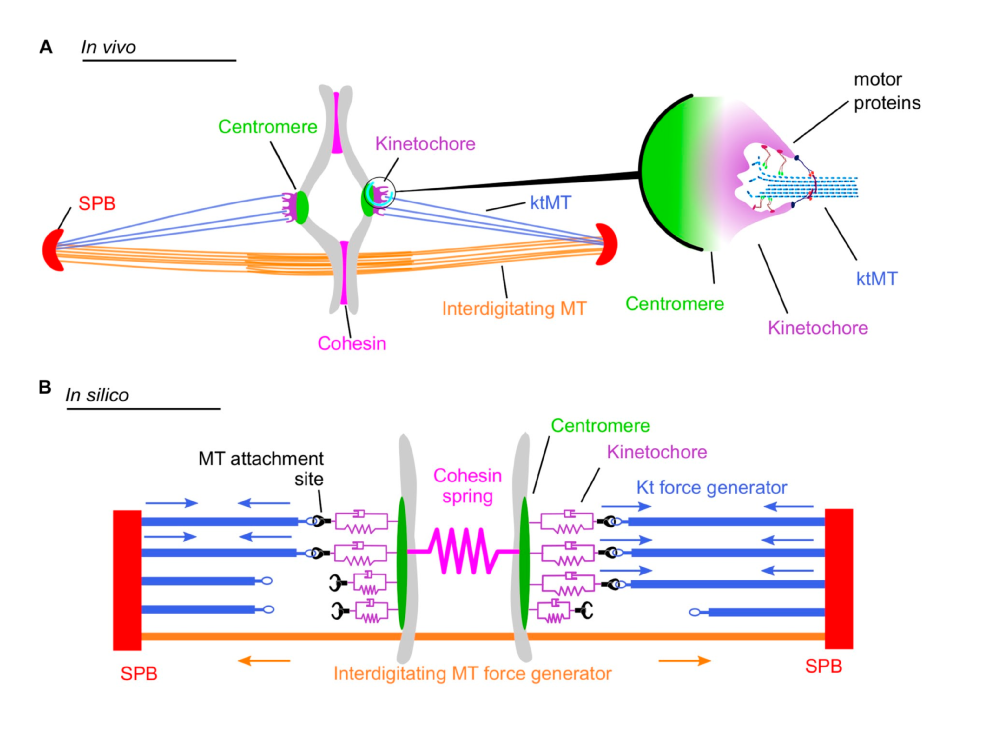
\includegraphics{figures/intro/gay.png}
\caption[Modèle de ségrégation des chromosomes]{\label{fig:gay}Modèle de
ségrégation des chromosomes basé sur un attachement KT-MT stochastique
(Gay et al., \hyperref[ref-Gay2012a]{2012}). \textbf{A}. Schéma du
fuseau mitotique de la levure à fission. \textbf{B}. Schéma du modèle
représentant la façon dont sont agencés les différents éléments
mécaniques du modèle reproduisant un fuseau mitotique \emph{in vivo}.}
\end{figure}

La même équipe proposa un peu plus tard un autre modèle plus général
décrivant la dynamique du fuseau de la prophase et l'anaphase (Gay et
al., \hyperref[ref-Gay2012a]{2012}). Ce modèle est composé d'objets
viscoélastiques représentant les composants du fuseau (pôle,
kinétochore, cohésine et site d'attachement). Chacune des ces unités est
arrangée de façon à former un fuseau (Figure~\ref{fig:gay}). Les sites
d'attachement sont autant de moteurs qui tirent le chromosome en
direction du pôle quand il est actif. Les attachements se désactivent de
manière stochastique, prenant également en compte deux mécanismes
régulant l'attachement KT-MT: l'orientation du kinétochore et la tension
exercée sur les deux kinétochores frères (Gay et al.,
\hyperref[ref-Gay2012a]{2012}).

Ce modèle décrit la dynamique du fuseau à un niveau macroscopique plus
haut que le modèle proposé par Civelekoglu-Scholey et al. L'une des
forces du modèle est sa capacité à décrire la dynamique des attachements
en métaphase et anaphase sans faire d'hypothèse forte sur le
fonctionnement de l'attachement et des différentes protéines participant
à ce processus. Les paramètres qui le composent résultent d'un grand
nombre de mesures \emph{in vivo} qui décrivent non pas des propriétés
individuelles de protéines mais des propriétés biophysiques d'objets
macroscopiques composant le fuseau telles que les constantes
d'élasticité du kinétochore ou d'un site d'attachement.

Un autre modèle de balance de force (Campàs and Sens,
\hyperref[ref-Campas2006]{2006}) adopte une approche simplifiée pour
décrire le mouvement des chromosomes monotéliques. Le mouvement est
principalement produit par des protéines motrices, les chromokinésines,
qui par l'intermédiaire des microtubules vont exercer une force sur les
bras des chromosomes, et ainsi générer une force dirigée dans la
direction opposée à celle du pôle.

Plus récemment, un troisième mécanisme alternatif fut proposé pour
expliquer l'attachement du microtubule au kinétochore. Ce modèle est une
adaptation de celui de Civelekoglu-Scholey et al.
(Figure~\ref{fig:hill_model}C). Le mécanisme est basé sur des
observations biophysiques d'un complexe protéique, appelé NDC80 et
supposé être responsable de l'attachement entre le microtubule et le
kinétochore (Alushin et al., \hyperref[ref-Alushin2010]{2010}; Joglekar
and DeLuca, \hyperref[ref-Joglekar2009]{2009}; Santaguida and Musacchio,
\hyperref[ref-Santaguida2009a]{2009}). En pratique ce modèle ressemble
au modèle de Hill proposé par Joglekar \& Hunt, à l'exception d'une
différence très importante: les liens élastiques peuvent se détacher et
s'attacher de manière indépendante les uns des autres
(Figure~\ref{fig:hill_model}C).

De plus, un mécanisme de « catch bond » est implémenté supposant qu'un
lien se détache plus facilement sous une faible tension plutôt que sous
une grande tension en agrément avec des mesures faites \emph{in vitro}
(Akiyoshi et al., \hyperref[ref-Akiyoshi2010]{2010}). Il en résulte que
les attachements avec un microtubule qui polymérise sont faibles tandis
que les attachements contenant un microtubule qui dépolymérise sont
forts.

La découverte d'une nouvelle structure responsable de l'attachement
KT-MT (Miranda et al., \hyperref[ref-Miranda2005]{2005}; Westermann et
al., \hyperref[ref-Westermann2005]{2005}), le complexe DAM1, a vu
apparaître des nouveaux modèles de l'attachement proposant le complexe
DAM1 comme coupleur principal entre le microtubule et le kinétochore
(Efremov et al., \hyperref[ref-Efremov2007]{2007}; McIntosh et al.,
\hyperref[ref-McIntosh2008]{2008}). Par exemple Efremov et al. ont
montré que la structure en anneau de DAM1 permet un couplage efficace,
qui peut fidèlement suivre un microtubule qui dépolymérise en captant
l'énergie libérée par les protofilaments incurvés (Efremov et al.,
\hyperref[ref-Efremov2007]{2007}). De plus cette association entre le
kinétochore et le complexe DAM1 a aussi été observée \emph{in vitro} par
électro-microscopie (McIntosh et al.,
\hyperref[ref-McIntosh2008]{2008}).

Une équipe propose un modèle de la dynamique des chromosomes chez la
levure à bourgeon (\emph{Saccharomyces cerevisiae}) dans lequel chaque
kinétochore ne peut contenir qu'un seul microtubule (Gardner et al.,
\hyperref[ref-Gardner2005]{2005}, \hyperref[ref-Gardner2008a]{2008}). Le
modèle mathématique prend en compte à la fois la régulation mécanique et
moléculaire de la dynamique de l'extrémité + du microtubule attachée au
kinétochore.

Il est bien entendu impossible de faire une liste exhaustive des modèles
décrivant la dynamique du fuseau. Cependant on retrouve un point
essentiel dans tout ces modèles : l'origine de l'énergie responsable du
mouvement des chromosomes reste encore très hypothétique. Pour résumer,
deux modèles existent : soit l'énergie provient de la dynamique du
microtubule (modèle de Hill), soit l'énergie provient de protéines
motrices (modèle de Civelekoglu-Scholey). On note qu'il est possible de
modéliser le fuseau mitotique sans aucune de ces deux hypothèses (Gay et
al., \hyperref[ref-Gay2012a]{2012}).

Pour une discussion plus détaillée sur les différents mécanismes capable
de générer une force au niveau du kinétochore, voir le commentaire de
Joglekar et al. (\hyperref[ref-Joglekar2010a]{2010}).

Dans un commentaire (McIntosh, \hyperref[ref-McIntosh2012]{2012}), J.
McIntosh souligne que ce problème de l'origine du mouvement des
chromosomes est encore incertain et que la solution est probablement
plus complexe qu'une origine unique pour tous les types de fuseaux et
d'organismes existants. Il propose cependant dans une revue (McIntosh et
al., \hyperref[ref-McIntosh2010]{2010}) que la dépolymérisation des
microtubules pourrait être un ancien moteur biologique responsable du
mouvement des chromosomes en soulignant deux choses. Chez certains
organismes comme la levure à fission, la délétion de toutes les
kinésines et dynéines, une par une, ne modifie pas la vitesse maximale
des chromosomes en mitose. De plus, une protéine similaire à la tubuline
existe chez la bactérie (appelé FtsZ) et contribue en grande partie à la
sa division (McIntosh et al., \hyperref[ref-McIntosh2010]{2010}).

\section{La levure à fission : un organisme modèle pour l'étude du cycle
cellulaire}\label{la-levure-uxe0-fission-un-organisme-moduxe8le-pour-luxe9tude-du-cycle-cellulaire}

La levure \emph{Schizosaccharomyces pombe} (Figure~\ref{fig:pombe}) est
une levure à division symétrique aussi appelée « levure à fission ».
Elle est de forme cylindrique de 3 à 4μm de diamètre et de 7 à 10μm de
longueur en fonction de l'étape du cycle cellulaire.

Elle se développe sur les racines des arbres ainsi que dans les sols à
proximité. On la retrouve aussi dans les vieux alcools. L'histoire
raconte que la levure à fission aurait été découverte dans un tonneau de
bière périmée (\emph{pombe} signifiant « dérivant de la bière »).

Depuis les années 50, les biologistes utilisent cette levure comme
organisme modèle afin d'étudier le cycle cellulaire et notamment la
mitose.

Elle possède trois chromosomes et une phase haploïde dominante (avec une
phase G2 très longue). La séquence de son génome a été publiée en 2002
par un consortium dirigé par l'Institut Sanger. On estime que son génome
contient environ 14 millions de paires de base codant pour
\textasciitilde{}5000 protéines et \textasciitilde{}500 ARNs non-codant.

\begin{figure}[htbp]
\centering
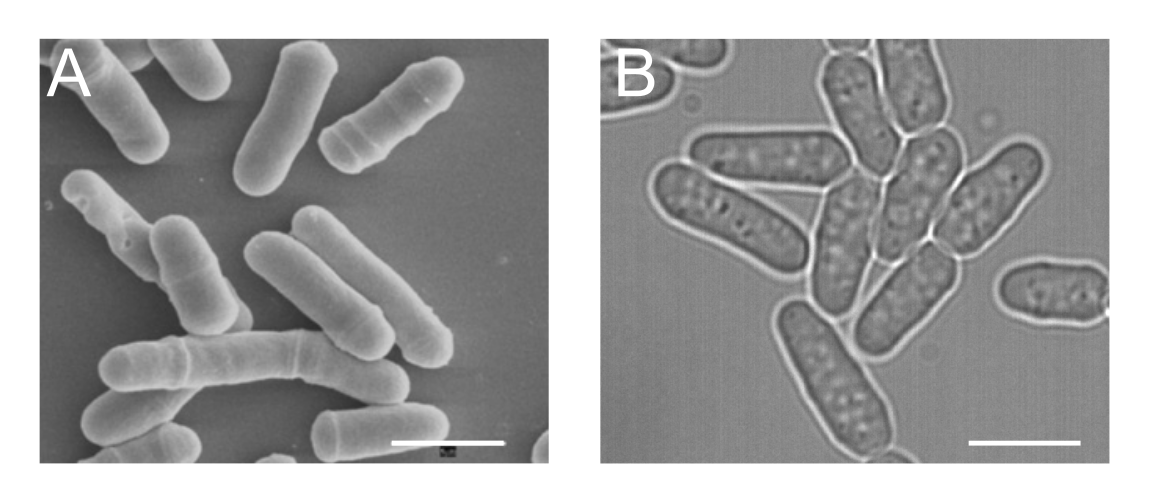
\includegraphics{figures/intro/pombe.png}
\caption[Morphologie de la levure à fission]{\label{fig:pombe}Morphologie
de la levure à fission. \textbf{A}. Vue en microscopie électronique à
balayage de \emph{S. pombe} (Morgan, \hyperref[ref-Morgan2007]{2007}).
\textbf{B}. Vue en microscopie optique à champ large en fond clair. La
barre correspond à 8 μm dans les deux vues.}
\end{figure}

Son cycle cellulaire classique est composé d'une phase G1 brève de 20mn,
d'une phase G2 longue de 2h et d'une phase de division (la mitose) qui
dure une vingtaine de minutes (Figure~\ref{fig:pombe-cell-cycle}). En
phase exponentielle de croissance, 80\% des cellules sont en G2 et
15-20\% en mitose.

\begin{figure}[htbp]
\centering
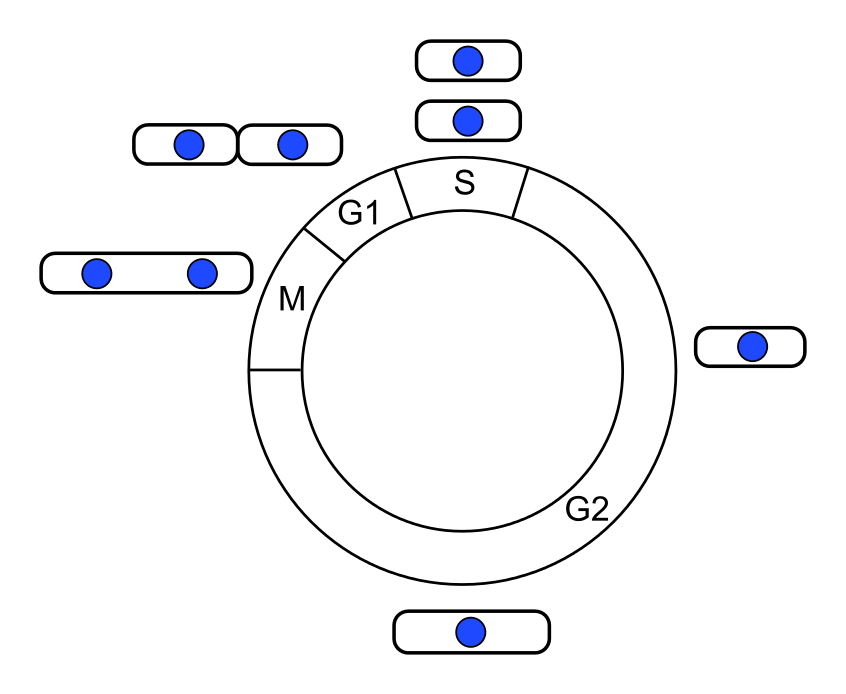
\includegraphics{figures/intro/pombe_cell_cycle.png}
\caption[Schéma du cycle cellulaire de la levure à fission]{\label{fig:pombe-cell-cycle}Schéma
du cycle cellulaire de la levure à fission. La levure à fission possède
une phase G2 très longue comparé à d'autres types cellulaire.}
\end{figure}

Bien que les principaux mécanismes gouvernant la mitose soient conservés
à la fois chez la levure à fission et chez les eucaryotes supérieurs,
quelques différences existent. La levure ne possède pas de centrosome
constituant les pôles du fuseau mitotique mais des structures appelées
SPB (« Spindle Pole Body » en anglais). La mitose de la levure est
fermée contrairement à de nombreuses cellules d'eucaryotes supérieurs,
c'est à dire que la division s'effectue dans le noyau.

Les phases de la mitose sont classiques et composées de la sorte : la
prométaphase qui dure 2.5min, où le fuseau va s'allonger jusqu'a
atteindre \textasciitilde{}2.5μm; la métaphase où le fuseau reste stable
grâce à un mécanisme de balance de force (Gay et al.,
\hyperref[ref-Gay2012a]{2012}), 2.5-3μm; l'anaphase A dure moins de 20s,
l'allongement du fuseau est rapide, de l'ordre de 0.5 à
1μm.min\textsuperscript{\textsuperscript{-1}} (Fu et al.,
\hyperref[ref-Fu2009]{2009}); enfin l'anaphase B qui dure
\textasciitilde{}10min où le fuseau va s'allonger jusqu'à atteindre la
taille de 5-6μm avant de lancer la cytocinèse. La cytocinèse s'effectue
par la contraction de l'anneau d'actine recruté au niveau du cortex de
la cellule.

Pour finir, la levure à fission est un puissant outil de biologie
moléculaire auquel il est aisé de supprimer, de manière conditionnelle
ou non, un gène ainsi que de marquer différentes protéines à l'aide de
marqueurs fluorescents.

En 1996, une équipe a mis au point un système permettant la
visualisation de la structure de la chromatine (Robinett,
\hyperref[ref-Robinett1996]{1996}). Cette technique, appelée système
LacO/LacI, consiste en l'insertion d'un grand nombre de répétitions
(plusieurs centaines) de l'opéron \emph{lac} (aussi appelée opéron
lactose) au sein du génome. Le gène \emph{lacI}, auquel a été ajoutée
une sonde fluorescente GFP, code pour le répresseur qui va venir se
fixer sur la partie du génome où a été inséré l'opéron \emph{lac}
(Figure~\ref{fig:lac}A). Ce système a été appliqué par une autre équipe
en 2003 afin de visualiser la partie péri-centromérique, proche du
kinétochore, du chromosome II de la levure à fission (Yamamoto and
Hiraoka, \hyperref[ref-Yamamoto2003]{2003}). Cette souche associée à un
marqueur fluorescent des pôles du fuseau permet donc la visualisation et
le suivi dans le temps de la position d'un chromosome au sein du fuseau
mitotique (Figure~\ref{fig:lac}B).

\begin{figure}[htbp]
\centering
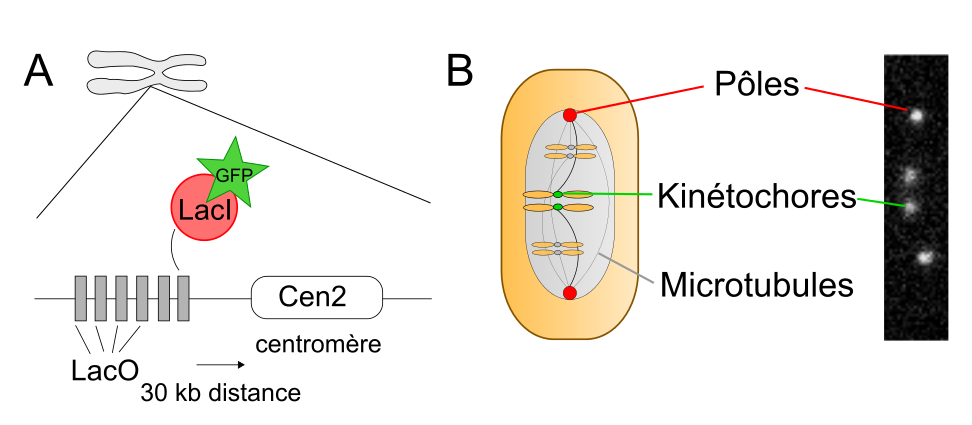
\includegraphics{figures/intro/lac.png}
\caption[Visualisation d'un seul chromosome en microscopie à fuorescence]{\label{fig:lac}Visualisation
d'un seul chromosome en microscopie à fuorescence. \textbf{A}. Système
LacO/LacI pour la visualisation d'une région spécifique d'un chromosome
à l'aide d'un marqueur fluorescent de type GFP. \textbf{B}. Schéma et
vue en microscopie à fluorescence d'une cellule de levure à fission
marquée pour les deux pôles du fuseau et les deux kinétochores du
chromosome II.}
\end{figure}

\emph{Schizosaccharomyces pombe} est donc devenu une référence dans
l'étude du cycle cellulaire. Cet organisme est très largement utilisé
par de nombreux biologistes afin de mieux comprendre les mécanismes
gouvernant et régulant la division cellulaire. Depuis quelques temps
maintenant, la levure à fission devient aussi un modèle de choix dans
l'étude des mécanismes biophysiques en jeu lors de la mitose.

\section{Problématique}\label{probluxe9matique}

L'approche biophysique dans l'étude de la mitose se justifie par le fait
que ce processus implique le mouvement de grands objets à l'échelle de
la cellule (les chromosomes) et donc l'existence de forces.

J'ai utilisé un ensemble de techniques provenant de différents domaines
scientifiques (physique, biologie et informatique) afin d'appréhender la
façon dont est régulée la dynamique des chromosomes durant la mitose.

Le terme « dynamique des chromosomes » est vaste et peut signifier
beaucoup de chose. Ici on entend par « dynamique des chromosomes »,
l'ensemble des processus qui gouvernent l'évolution spatiale et
structurelle des chromosomes tout au long de la mitose.

Plus précisément, ce travail a pour objectif d'étudier la régulation de
la congression des chromosomes en fonction du mouvement des kinétochores
durant la métaphase.

Pour cela, j'ai utilisé des souches de levures marquées pour les deux
pôles du fuseau ainsi que les deux kinétochores du chromosome II. Les
kinétochores sont ensuite observés en temps réel à l'aide d'un
microscope à fluorescence à champ large, durant la mitose, afin de
suivre, à différents intervalles de temps, leur position le long de
l'axe du fuseau mitotique.

Des analyses informatiques combinées à des techniques d'imagerie ont
ensuite permis d'extraire de manière automatique et reproductible la
position des kinétochores afin de reconstruire leurs trajectoires au
cours du temps. Les trajectoires ont ensuite été analysées par des
techniques provenant de l'analyse du signal afin d'en extraire les
principales propriétés.

Enfin un modèle mathématique de la mitose (Gay et al.,
\hyperref[ref-Gay2012a]{2012}) a été utilisé afin de tester plusieurs
hypothèses de mécanismes à l'origine de la congression ainsi que les
mécanismes gouvernant le mouvement des chromosomes.

\chapter{Résultats}\label{ruxe9sultats}

\section{« Fission yeast kinesin-8 controls chromosome congression
independently of oscillations »}\label{sec:article}

Chez les eucaryotes supérieurs, la congression des chromosomes dépend
entre autre de l'activité des chromokinésines. Cette étude analyse de
manière quantitative l'oscillation et le positionnement des chromosomes
dans la levure à fission (\emph{S. pombe}), un organisme modèle qui ne
possède pas de chromokinésine.

Dans des cellules sauvages, les chromosomes s'alignent durant la
prophase et tout en oscillant maintiennent leur alignement jusqu'à la
métaphase. L'oscillation des chromosomes n'est pas indispensable à
l'alignement des chromosomes en métaphase.

Chez les eucaryotes supérieurs, la kinésine 8 contrôle la congression
des chromosomes en régulant leurs oscillations. De manière opposée, nous
montrons que la kinésine 8 de la levure à fission contrôle la
congression des chromosomes par un mécanisme alternatif. Nous proposons
que la kinésine 8 aligne les chromosomes en contrôlant les forces de
traction en fonction de la longueur des microtubules attachés aux
chromosomes.

De plus un modèle mathématique de la ségrégation des chromosomes
implémentant ce mécanisme dépendant de la longueur est suffisant pour
reproduire l'alignement des chromosomes et prévenir l'apparition de
chromosomes retardataires en anaphase.

Dans l'ensemble, ces données illustrent comment l'action locale d'une
protéine motrice au kinétochore peut fournir une information spatiale à
l'ensemble de fuseau afin de permettre l'alignement des chromosomes.

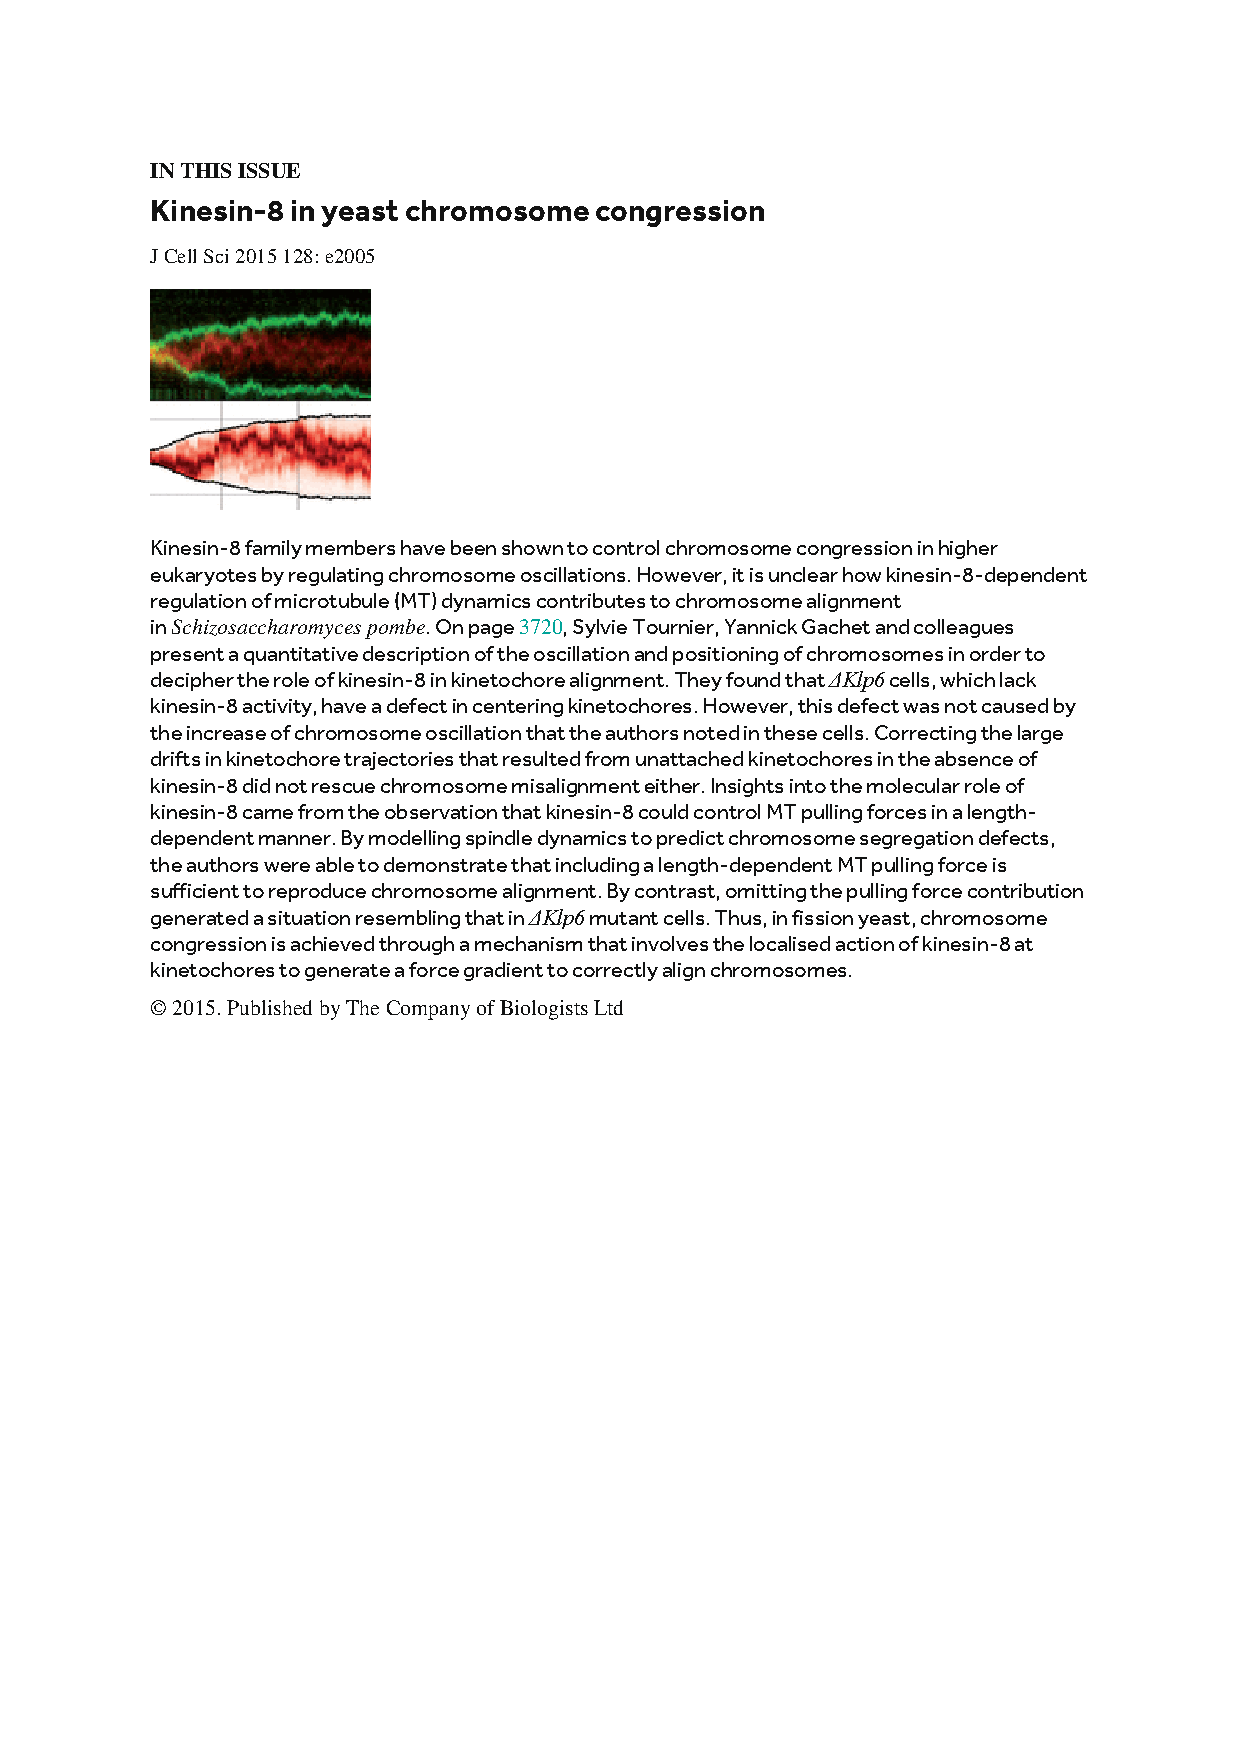
\includepdf[pages=-,pagecommand=\thispagestyle{plain}]{text/3_resultats/jcs_issue.pdf}
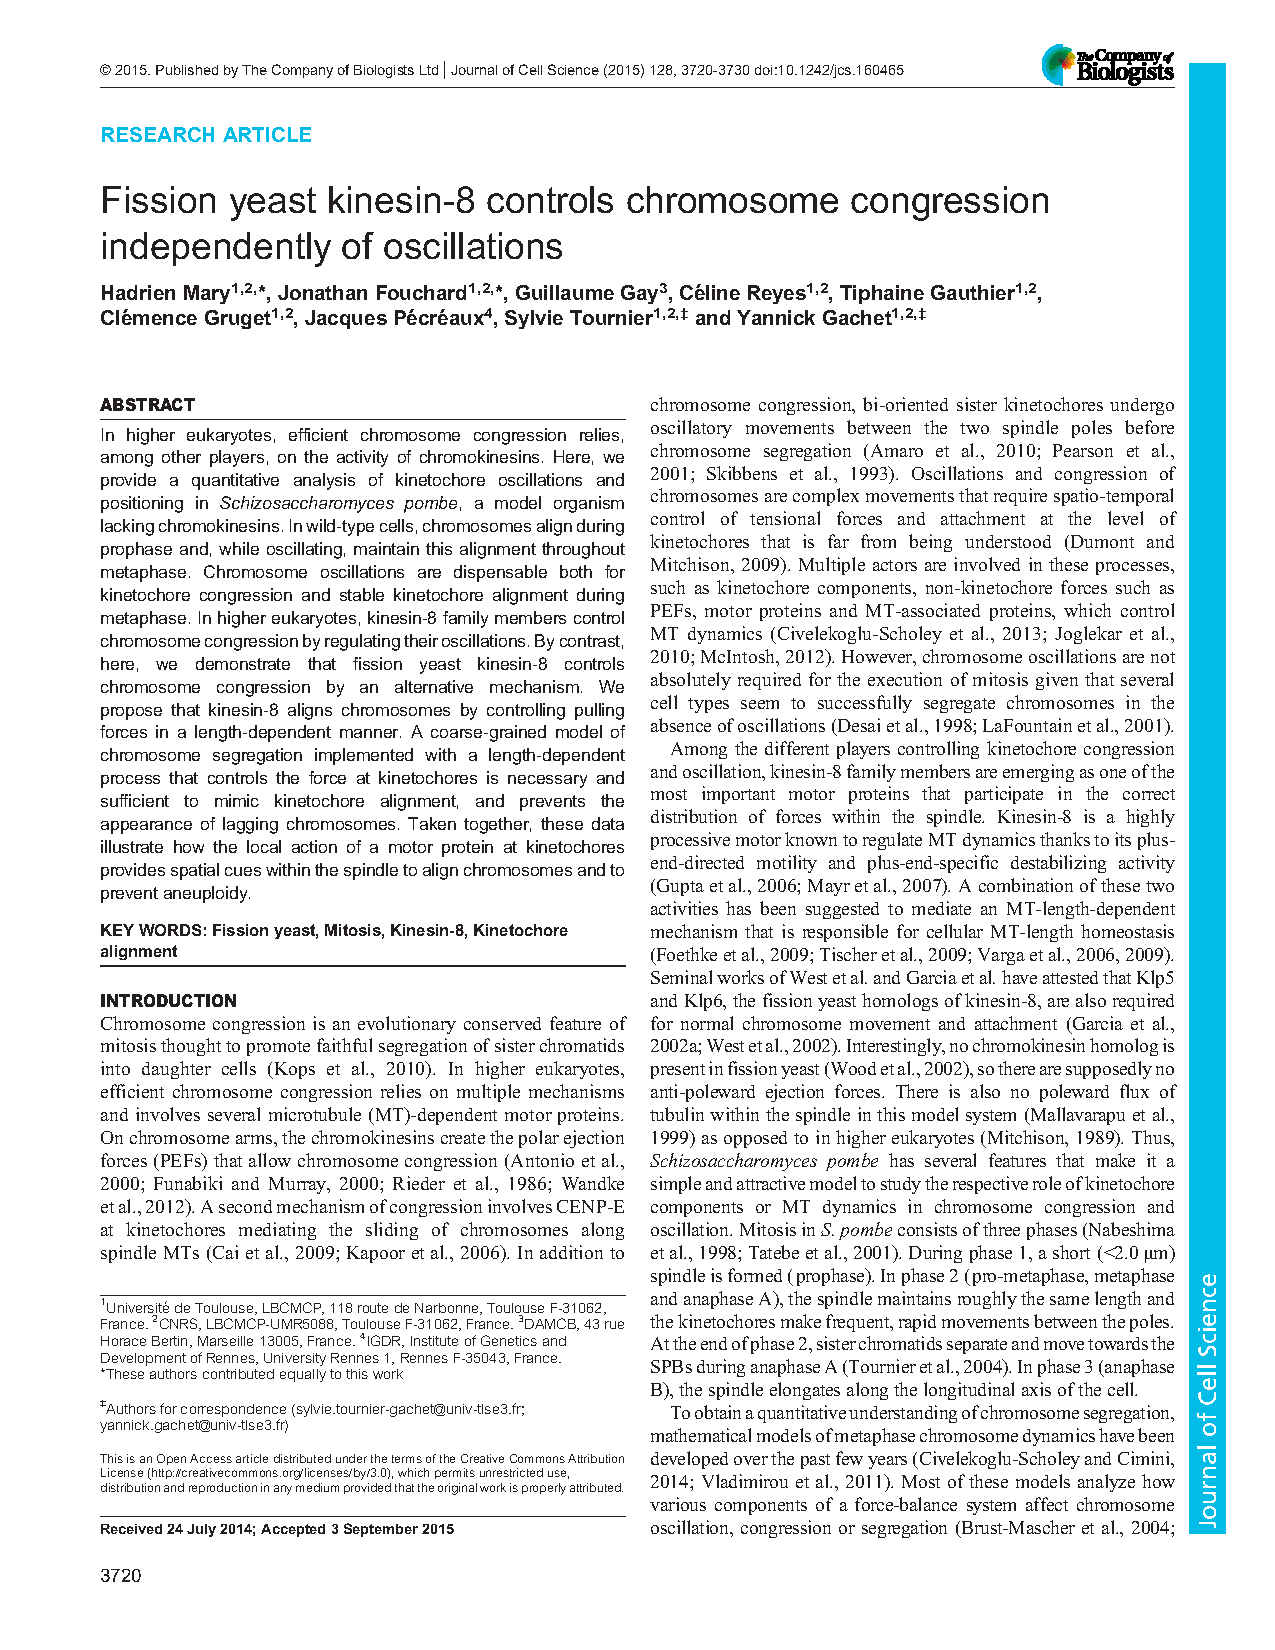
\includepdf[pages=-,pagecommand=\thispagestyle{plain}]{text/3_resultats/jcs_article.pdf}
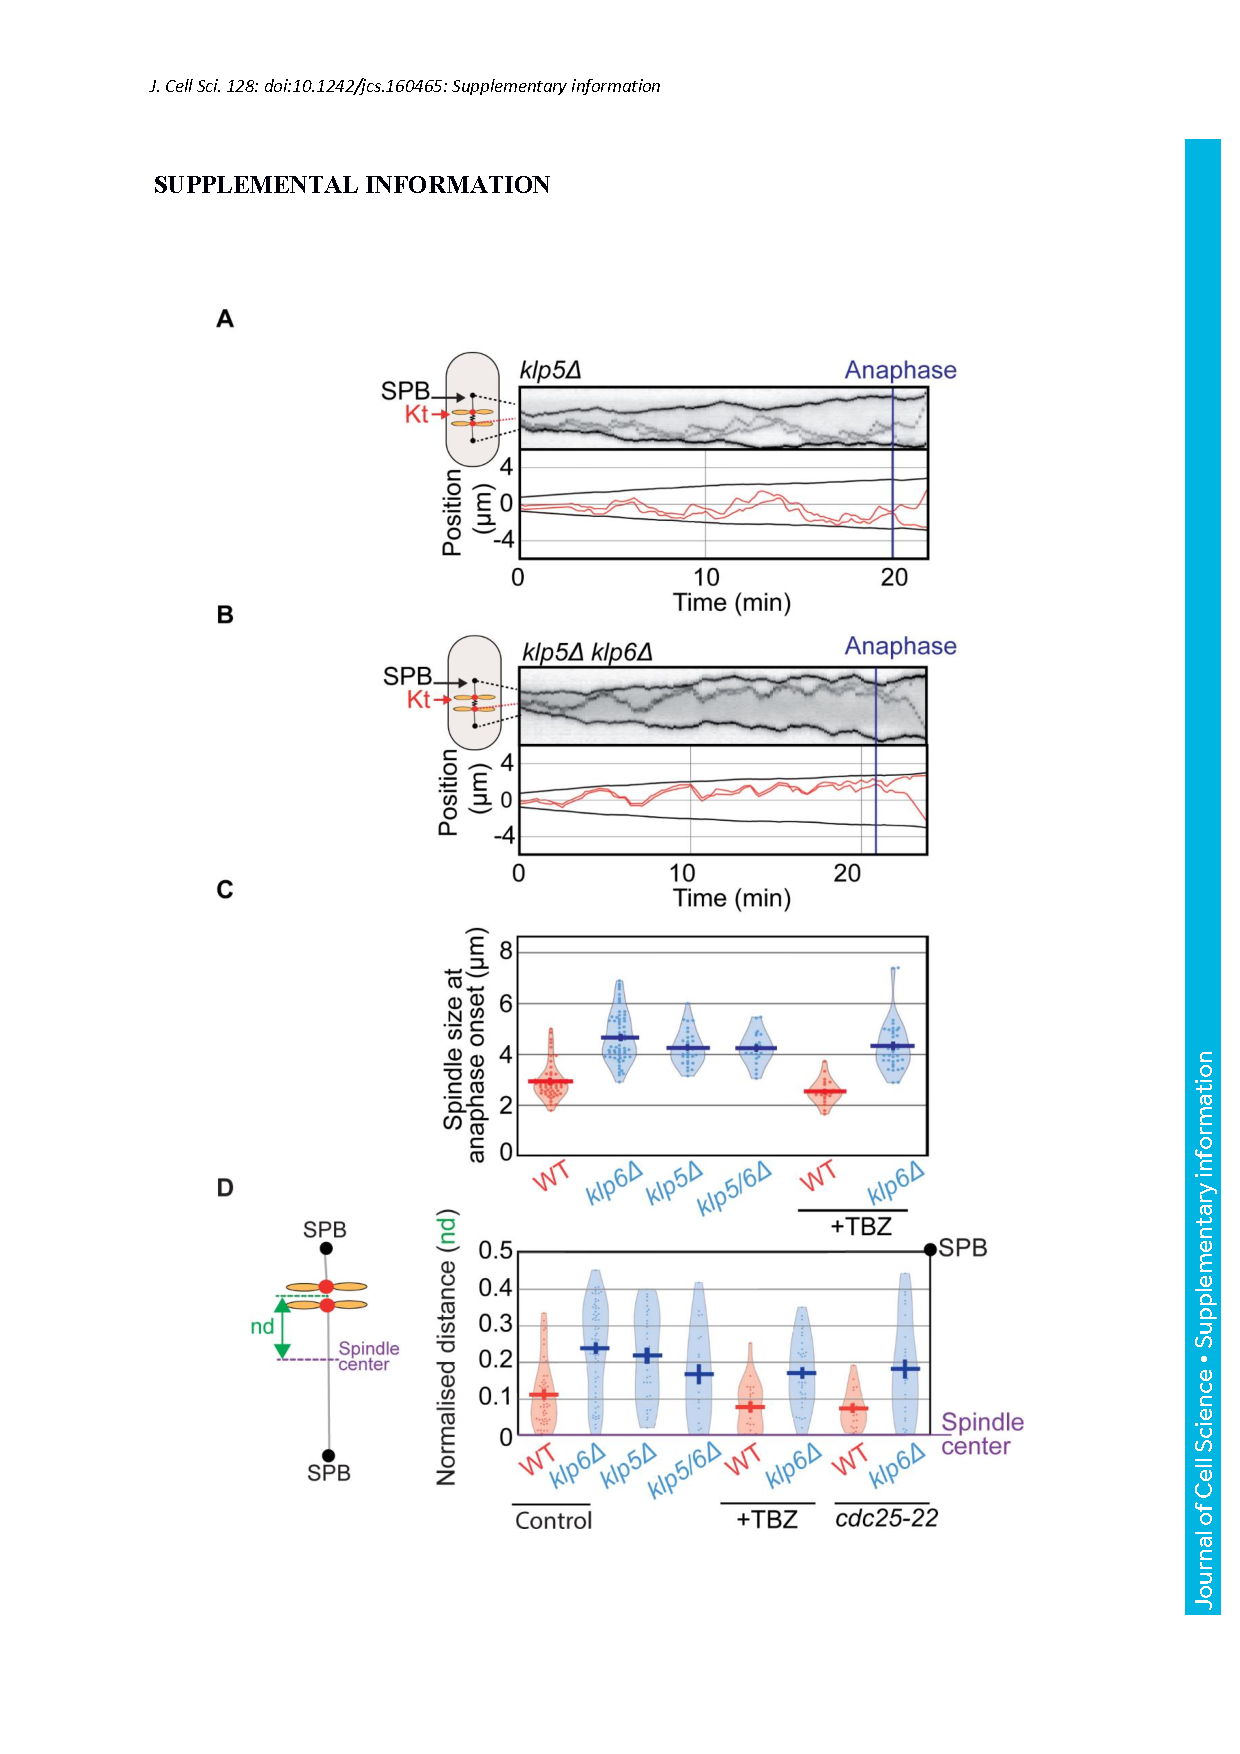
\includepdf[pages=-,pagecommand=\thispagestyle{plain}]{text/3_resultats/jcs_supp.pdf}

\section{Reconstruction et analyse de la trajectoire des chromosomes en
métaphase}\label{reconstruction-et-analyse-de-la-trajectoire-des-chromosomes-en-muxe9taphase}

L'analyse des mouvements des chromosomes permet d'inférer les mécanismes
régulant la dynamique du fuseau mitotique. En effet l'ensemble des
interactions physico-chimiques des toutes les molécules et protéines
composant le fuseau permet l'émergence de phénomènes de plus haut niveau
comme le mouvement et l'attachement des chromosomes durant la mitose.
Tout ces mécanismes sont requis pour une division cellulaire stable et
fidèle.

L'analyse du mouvement se déroule en trois étapes et peut être
appliquées à un grand nombre de type de cellules différentes :

\begin{itemize}
\item
  Avant l'étape d'acquisition, il est nécessaire de générer des lignées
  cellulaires dont les kinétochores ou bien la partie centromérique de
  la chromatide d'un ou de plusieurs chromosomes sont marqués avec une
  sonde fluorescente. L'acquisition se déroule généralement à l'aide
  d'un microscope à champs large ou confocal dont on règle les
  paramètres d'acquisition afin d'obtenir une photo des cellules à des
  pas de temps définis. Plus le pas de temps est faible, plus large sera
  l'éventail des phénomènes biophysiques observables. Cependant, des pas
  de temps trop faibles sur des durées trop longues auront tendance à
  endommager les cellules par la phototoxicité.
\item
  L'étape de reconstruction de la trajectoire des chromosomes comprend
  la détection des différents éléments observés (souvent kinétochore et
  pôle du fuseau mitotique) pour chaque pas de temps suivi de la
  jointure des objets détectés dans le temps.
\item
  Enfin la dernière étape d'analyse proprement dite n'est pas aussi bien
  défini que les deux étapes précédentes. Elle consiste à utiliser
  différents outils ou algorithmes afin de comparer et d'analyser les
  propriétés des trajectoires reconstruites pour en déduire différents
  mécanismes régulant la dynamique des chromosomes.
\end{itemize}

Cette stratégie d'analyse a été appliquée dans l'étude présentée en
Section~\ref{sec:article}. Ce qui suit propose de détailler les
différents outils utilisés ainsi que de présenter de nouvelles
techniques d'analyse.

\subsection{La reconstruction des trois chromosomes de la levure à
fission : un challenge
?}\label{la-reconstruction-des-trois-chromosomes-de-la-levure-uxe0-fission-un-challenge}

Après l'acquisition en vidéo-microscopie, la première étape consiste
donc à détecter chacun des spots qui correspond à un kinétochore ou à un
des deux pôles du fuseau mitotique.

La résolution de la vidéo-microscopie actuelle ainsi que la taille du
fuseau mitotique de la levure à fission (entre 1 et 4μm) rend la
différenciation entre les six kinétochores très difficile tout au long
de la métaphase (Figure~\ref{fig:spindle_peaks}A).

Il est possible de visualiser uniquement un chromosome en utilisant une
sonde fluorophore située sur une zone spécifique de ce chromosome au
niveau de sa partie péri-centromérique. Une lignée pré-existante
(Yamamoto and Hiraoka, \hyperref[ref-Yamamoto2003]{2003}) a donc été
utilisée afin de marquer le chromosome II de la levure à fission à
l'aide d'un système LacO/LacI (Robinett,
\hyperref[ref-Robinett1996]{1996}). Cette lignée permet une
différenciation beaucoup plus facile entre les deux kinétochores du
chromosome visualisé (Figure~\ref{fig:spindle_peaks}B).

\begin{figure}[htbp]
\centering
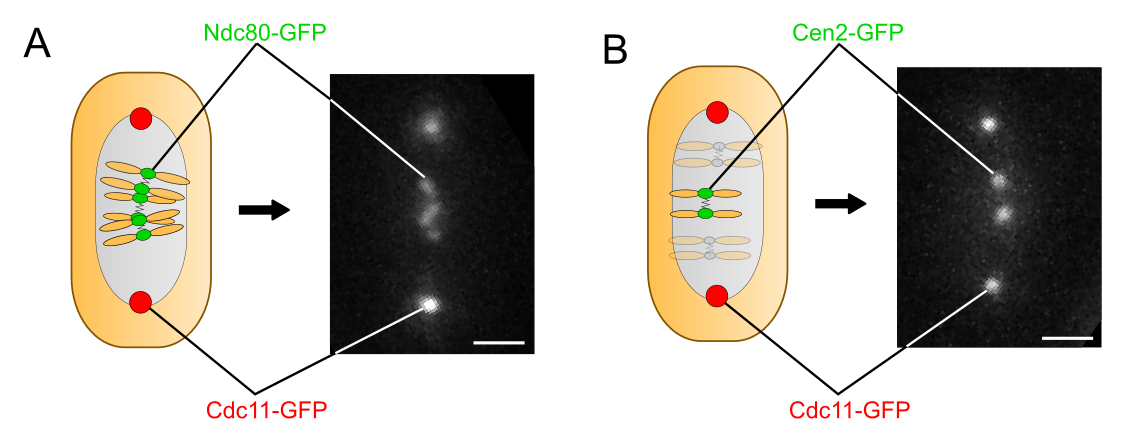
\includegraphics{figures/results/imaging/spindle_peaks.png}
\caption[Image en microscopie à fluorescence de deux fuseaux mitotique]{\label{fig:spindle_peaks}Image
en microscopie à fluorescence de deux fuseaux mitotiques. \textbf{A}.
Cellule marqué en GFP pour les six kinétochores (Ndc80-GFP, en vert sur
le schéma) et pour les pôles (Cdc11-GFP, en rouge sur le schéma).
\textbf{B}. Cellule marqué en GFP pour le centromère du chromosome II
(Cen2-GFP, en vert sur le schéma) et pour les pôles (Cdc11-GFP, en rouge
sur le schéma). La barre d'échelle correspond à 1μm.}
\end{figure}

De l'information est donc perdue (la position des kinétochores des deux
autres chromosomes) au profit d'une précision très fortement accrue de
la position des deux kinétochores restant.

Enfin on remarque que la visualisation des pôles se fait dans la même
longueur d'onde que les kinétochores (marqués en GFP) afin de ne pas
avoir à imager dans deux longueurs d'ondes différentes dans le but de
réduire les dommages causés par la phototoxicité du système
d'acquisition ainsi que de réduire le temps d'intervalle minimal entre
deux acquisitions.

\subsubsection{Détection par fit
gaussien}\label{duxe9tection-par-fit-gaussien}

En imagerie on définit un blob comme étant « une région d'une image
formée par un ensemble de pixels connectés spatialement ». Plus
communément un blob est un point qui correspond à une région
intéressante de l'image. Par exemple, la Figure~\ref{fig:spindle_peaks}B
contient quatre blobs, deux correspondant aux pôles du fuseau mitotique
et deux autres correspondant à la partie péri-centromérique des deux
chromatides sœurs du chromosome II. L'étape de la détection est
d'arriver à obtenir les propriétés géométriques de ces quatre objets
(position, largeur et intensité).

L'un des algorithmes les plus utilisés pour la détection de blob se base
sur la convolution de l'image par un noyau Gaussien suivi de
l'application de l'opérateur Laplacien (on parle de « Laplacian of
Gaussian »). Cette approche est très précise mais est aussi très
sensible au paramètre d'échelle, c'est à dire que son résultat va
fortement dépendre de la relation entre la taille des structures des
blobs et la taille du noyau gaussien.

L'idée de convoluer l'image source avec un noyau gaussien vient de
l'observation que les blobs des sondes utilisées en biologie peuvent
parfois avoir une forme qui s'approche d'une distribution gaussienne en
deux dimensions (Figure~\ref{fig:gaussian}).

La qualité de la détection dépend aussi de la qualité du rapport
signal/bruit de l'image ainsi que de la fidélité de la sonde
fluorescente à reproduire une distribution gaussienne. Par exemple on
peut remarquer que la sonde Cen2-GFP (Figure~\ref{fig:gaussian}B)
possède souvent une gaussienne moins bien définie que la sonde Cdc11-GFP
(Figure~\ref{fig:gaussian}C)). Ceci pourrait être causé par le fait que
la sonde Cen2-GFP consiste en une répétition d'insertion d'un gène
(LacO) le long de la partie péri-centromérique du chromosome II. Il en
résulterait un signal moins centré autour d'un unique point de l'espace
et plus diffus sur la longueur du chromosome.

\begin{figure}[htbp]
\centering
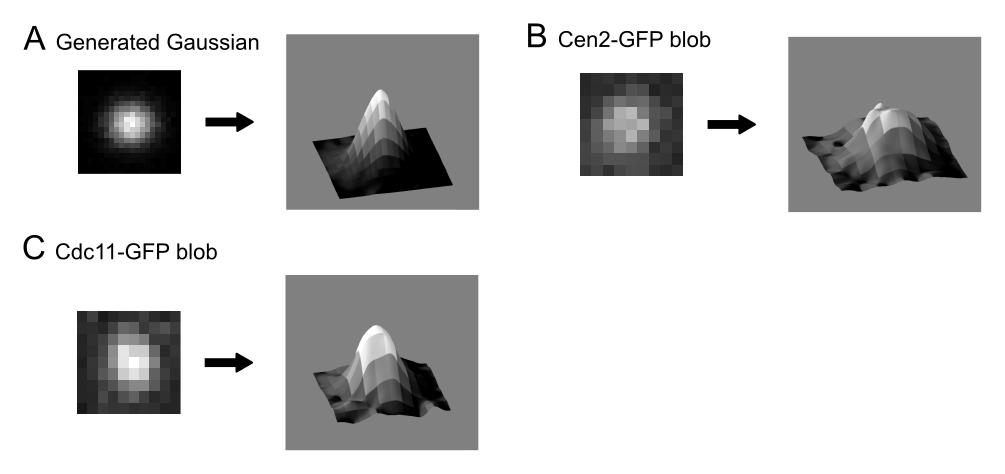
\includegraphics{figures/results/imaging/gaussian.png}
\caption[Distribution des intensités gaussiennes en deux dimensions]{\label{fig:gaussian}Distribution
des intensités gaussiennes en deux dimensions. \textbf{A}. Cette image a
été générée \emph{in silico} par l'échantillonnage aléatoire d'une
distribution gaussienne. Le surface plot (image de droite) contient une
dimension supplémentaire en \(z\) dont la hauteur est proportionnelle à
l'intensité des pixels dans l'image originale (image de gauche) .
\textbf{B}. Cette image correspond à un blob de la sonde Cen2-GFP qui
marque le centromère d'une des chromatides du chromosome II. \textbf{C}.
Cette image correspond à un blob de la sonde Cdc11-GFP qui marque les
deux pôles du fuseau mitotique.}
\end{figure}

Une implémentation existe dans le plugin TrackMate inclus dans Fiji
(Schindelin et al., \hyperref[ref-Schindelin2012]{2012}). Son code est
librement disponible.\footnote{\url{http://git.io/vC9zf}}

Cette implémentation a été utilisée pour l'analyse des images de
vidéo-microscopie durant ce travail. La précision de la détection a
aussi été testée en détectant des faux films générés depuis des
trajectoires simulées \emph{in silico}
(Figure~\ref{fig:detection_precision}A). La distance entre la position
réelle \emph{in silico} puis la position détectée a ensuite été comparée
(Figure~\ref{fig:detection_precision}B). La largeur à mi hauteur (FWHM,
\emph{full width at half maximum}) de la distribution de l'erreur de
détection est d'à peu près 34nm.

\begin{figure}[htbp]
\centering
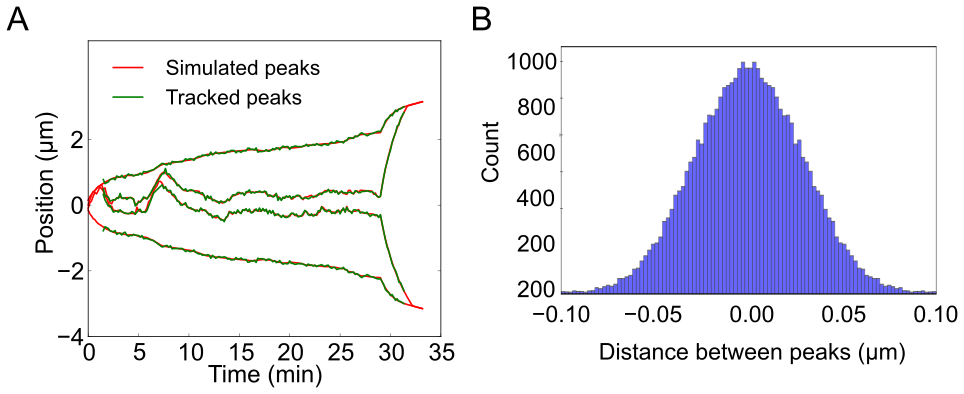
\includegraphics{figures/results/imaging/detection_precision.png}
\caption[Précision de la détection des blobs]{\label{fig:detection_precision}Précision
de la détection des blobs. \textbf{A}. Superposition d'une trajectoire
de chromosome et pôle simulée \emph{in silico} (en rouge) avec la
trajectoire reconstruire par détection de blob (en vert). \textbf{B}.
Distribution de la distance entre les blobs simulés et les blobs
détectés.}
\end{figure}

Enfin un autre algorithme de détection de blob a aussi été testé durant
ce travail. Il est basé sur le travail de Sergé et al. (Sergé et al.,
\hyperref[ref-Serge2008]{2008}) dont le principal atout consiste à être
capable de détecter plusieurs blobs très proches les uns des autres
comme cela peut être le cas lorsque l'on visualise les six kinétochores
de la levure à fission (Figure~\ref{fig:spindle_peaks}A).

L'idée principale est d'appliquer un algorithme de détection de blob
plusieurs fois. Entre chaque tour de détection, on soustrait les blobs
détectés à l'image source et on re-détecte les blobs restant
(Figure~\ref{fig:deflation}). L'algorithme s'arrête quand plus aucun
blob n'est détecté dans l'image. Cela permet la détection des blobs
d'intensité plus faible qui sont masqués par celui de plus forte
intensité situé à proximité.

\begin{figure}[htbp]
\centering
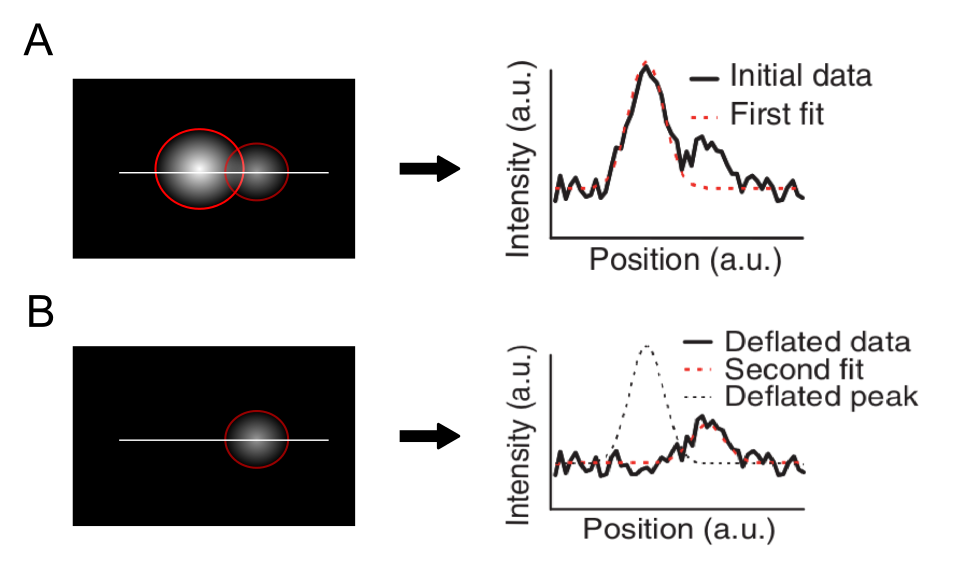
\includegraphics{figures/results/imaging/deflation.png}
\caption[Principe de l'algorithme de détection de blob par déflation]{\label{fig:deflation}Principe
de l'algorithme de détection de blob par déflation. \textbf{A}. Le
premier tour de fit gaussien détecte le blob le plus grand et le plus
intense. \textbf{B}. Une fois le premier blob détecté soustrait de
l'image source, le second tour de fit gaussien détecte le blob plus
petit et moins intense. Les line plots situés à droite des schémas sont
adaptés de Sergé et al. (\hyperref[ref-Serge2008]{2008}).}
\end{figure}

Une implémentation en Python de cet algorithme est librement disponible
en ligne.\footnote{\url{http://git.io/vCHGs}}

Deux raisons ont empêchés cet algorithme d'être utilisé dans le cadre de
ce travail. La première est que l'implémentation en Python est beaucoup
plus lente (quasiment un facteur 100) que la détection de blob proposée
par le plugin TrackMate. Afin de remédier à cela il faudrait
ré-implémenter l'algorithme de façon plus efficace, probablement en
utilisant un langage plus bas niveau tel que Cython ou le C. Cette perte
de temps aurait pu éventuellement être acceptable si la détection de
blobs superposés dans les images à six kinétochores
(Figure~\ref{fig:spindle_peaks}A) fonctionnait bien. Or l'algorithme de
déflation ne donne pas de résultat convaincant comparé à celui proposé
par TrackMate (Figure~\ref{fig:compare}). Ceci pourrait s'expliquer par
le fait que la déflation est réellement efficace sur des sondes à
molécules unique (« Single Particle Tracking » ou aussi SPT en anglais)
et non pas des agrégats de multiples sondes fluorophores comme c'est le
cas pour Cen2-GFP.

\begin{figure}[htbp]
\centering
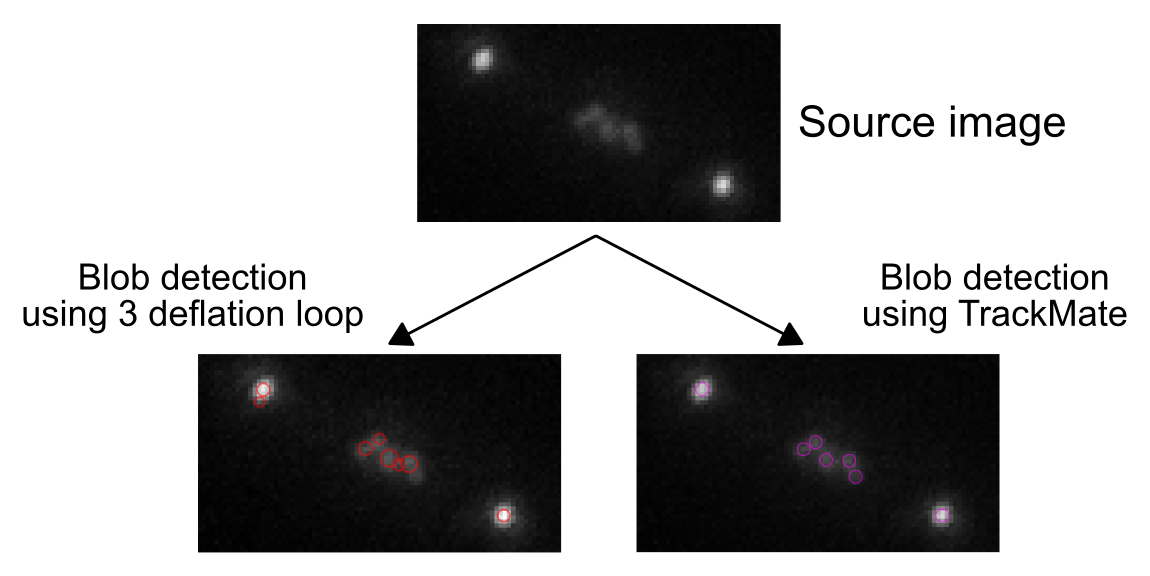
\includegraphics{figures/results/imaging/compare.png}
\caption[Principe de l'algorithme de détection de blob par déflation]{\label{fig:compare}Comparaison
entre le LoG détection de TrackMate et l'implémentation par déflation
basé sur l'algorithme de Sergé et al. Aucun des deux algorithmes
n'arrivent à détecter les six kinétochores et les deux pôles. Par contre
l'algorithme de TrackMate (à droite) détecte cinq kinétochores et les
deux pôles. Alors que l'autre algorithme (à gauche) fait plus d'erreurs
en détectant deux pôles au lieu de un (en haut) et en omettant un
kinétochore au milieu.}
\end{figure}

Une fois les blobs détectés pour chaque pas de temps, il faut encore
relier chaque blob avec son blob correspondant dans le temps afin
d'obtenir les trajectoires uniques de chaque chromosomes et des pôles;
c'est l'étape de tracking.

\subsubsection{Reconstruction des
trajectoires}\label{reconstruction-des-trajectoires}

Durant le tracking, les trajectoires des objets observés (les
chromosomes et les pôles) sont reconstruites. C'est à dire que chaque
blob est relié avec le blob qui correspond au même objet dans tout les
pas de temps (Figure~\ref{fig:whatistracking}).

\begin{figure}[htbp]
\centering
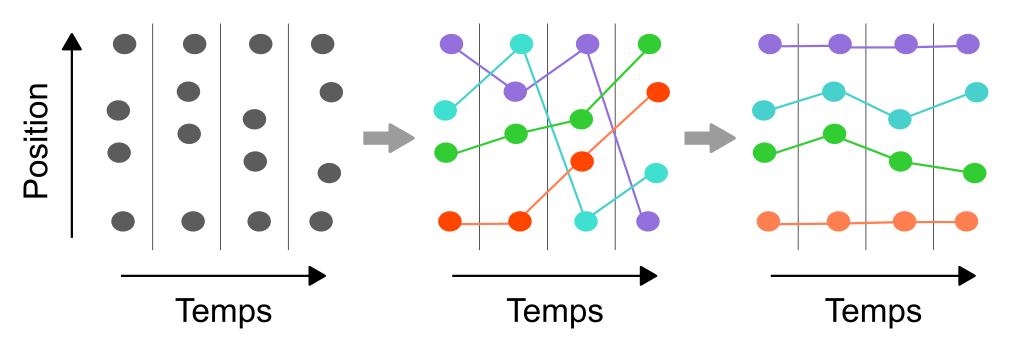
\includegraphics{figures/results/imaging/whatistracking.png}
\caption[Le tracking est l'étape de liaison des objets d'intérêts dans le temps]{\label{fig:whatistracking}Le
tracking est l'étape de liaison des objets d'intérêts dans le temps.
Sans cette étape il est impossible de savoir si un objet est le même
qu'un autre dans deux temps différents.}
\end{figure}

Tout les algorithmes de tracking sont basés sur la même idée que d'un
pas de temps à l'autre, deux blobs correspondent au même objet si leurs
distances est la plus petite parmi toutes les distances possibles avec
les autres blobs.

Le tracking consiste donc à minimiser un ensemble de solutions parmi le
champ des possibles. La version la plus utilisée se base sur la
minimisation de la distance euclidienne d'un pas de temps à l'autre.

\paragraph{Trois chromosomes}\label{trois-chromosomes}

Le tracking des six kinétochores est un challenge. En effet comme déjà
vu en Figure~\ref{fig:spindle_peaks}A, les six kinétochores évoluent
ensemble dans un espace de petite taille, le fuseau mitotique. De plus
ils ont tendance à se superposer très souvent. On notera qu'il n'est pas
possible de les différencier même en filmant dans la profondeur du
champs focal (en \(z\)).

Cependant il est possible de reconstruire partiellement des morceaux de
trajectoires. Pour cela il est possible d'utiliser un framework général
de tracking de particules développé par Jaqaman et al. appelé le LAP
tracker pour \emph{Linear Assignement Problem tracker} (Jaqaman et al.
(\hyperref[ref-Jaqaman2008]{2008})).

L'idée du LAP tracker est de minimiser successivement deux matrices de
coût contenant l'ensemble des solutions possibles au problème
(Figure~\ref{fig:jaqaman}).

\begin{figure}[htbp]
\centering
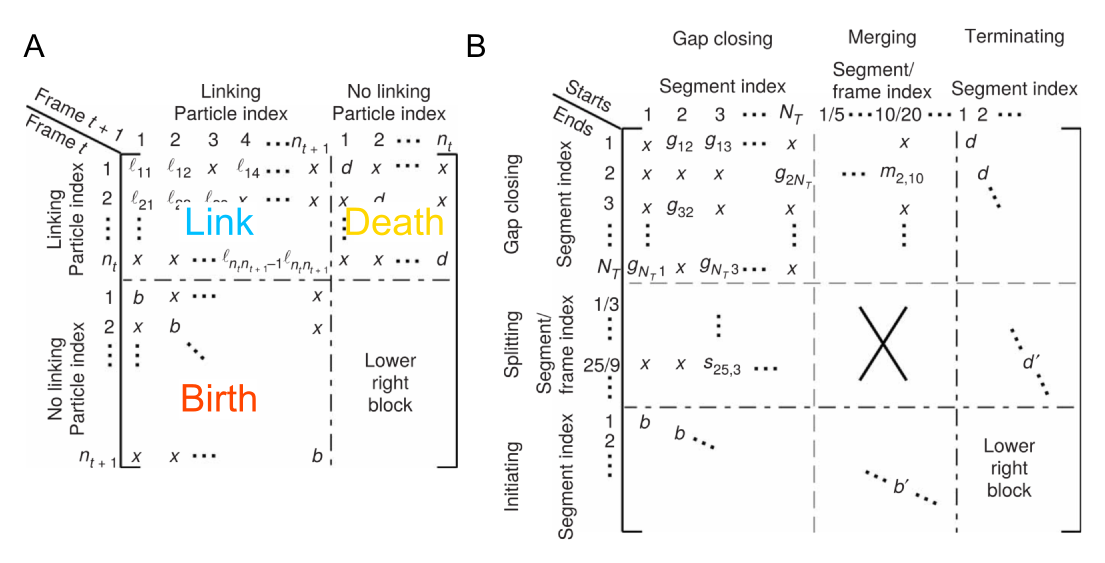
\includegraphics{figures/results/imaging/jaqaman.png}
\caption[Les deux matrices de coût du LAP tracker]{\label{fig:jaqaman}Les
deux matrices de coût du LAP tracker. \textbf{A}. Matrice de coût
contentant l'ensemble des liens possibles entre deux blobs pour deux pas
de temps successifs \(t\) et \(t+1\). Il existe donc autant de cette
première matrice que de pas de temps dans la trajectoire. Le bloc en bas
à droite (LRB) est un bloc auxiliaire requis pour satisfaire des
contraintes topologiques de l'algorithme. \textbf{B}. Matrice de coût
contrôlant la fermeture des trous, la fusion et la séparation des
trajectoires. Adapté de Jaqaman et al.
(\hyperref[ref-Jaqaman2008]{2008}).}
\end{figure}

Dans la première matrice (Figure~\ref{fig:jaqaman}A), chaque ligne et
colonne correspond à un blob allant de de \(1\) à \(n_{t+1}\) pour deux
pas de temps successifs \(t\) et \(t+1\). Chaque intersection de la
matrice va contenir un score qui va mesurer la probabilité que
l'événement en question arrive. Par exemple pour le bloc en haut à
gauche (le bloc de liaison), chaque case correspond à un événement de
liaison entre les deux blobs correspondant. Tandis que dans le bloc en
bas à gauche, le score correspond à la probabilité que ce blob soit le
premier d'une trajectoire (c'est à dire qu'il n'est lié a aucun autre
blob dans le passé), on parle alors de « birth ». Le bloc en haut à
droite correspond aux probabilités de mort d'une trajectoire, c'est à
dire que le blob soit le dernier d'une trajectoire (pas de liaison dans
le futur), on parle alors de « death ».

Le score du bloc de liaison peut être défini de plusieurs manières. Si
on suppose un mouvement brownien on peut simplement définir le score
comme la distance au carré qui séparent les deux particules. Si on
étudie un mouvement dirigé on peut utiliser par exemple un score basé
sur la distance entre le blob \(t+1\) et une position prédite et
probable qui correspondrait à un mouvement dirigé (basé sur un filtre de
Kalman par exemple).

Une fois les matrices crées (on note qu'il existe \(t-1\) matrices dans
le cas de la première matrice). Elles sont minimisés en utilisant
l'algorithme de Jonker-Volgenant (Jonker and Volgenant
(\hyperref[ref-Jonker1987]{1987})). La minimisation des matrices va
alors calculer la combinaison des événements les plus probables en se
basant sur les scores. On obtient ainsi des trajectoires.

La seconde matrice (Figure~\ref{fig:jaqaman}B) gère des événements plus
complexes liés aux trajectoires et non plus aux blobs. Ici chaque ligne
et colonne correspond à une trajectoire. Le calcul des scores cherche à
exprimer la probabilité d'événements tel que le lien entre le début
d'une trajectoire et la fin d'une autre, la fusion ou la séparation de
deux trajectoires.

Deux implémentations ont été testées (Figure~\ref{fig:ndc80}). La
première provenant d'un module Python crée pour l'occasion, appelé
\texttt{scikit-tracker}, possédant une fonction de score supposant un
mouvement brownien (Figure~\ref{fig:ndc80}A). La seconde est celle
disponible dans TrackMate et contient une fonction de score qui suppose
un mouvement dirigé basé sur un filtre de Kalman pour prédire les
trajectoires (Figure~\ref{fig:ndc80}B).

\begin{figure}[htbp]
\centering
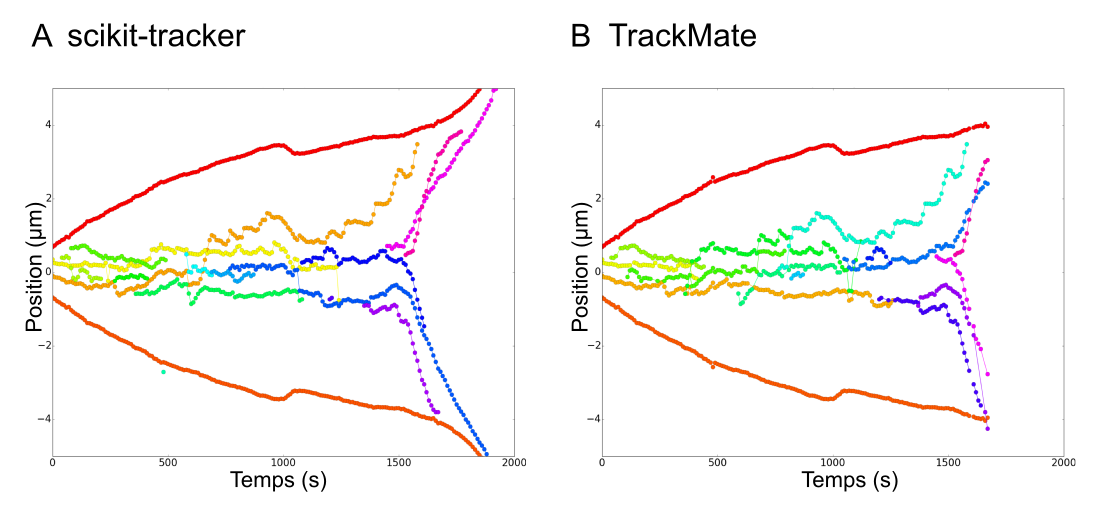
\includegraphics{figures/results/imaging/ndc80.png}
\caption[Reconstruction de la trajectoire avec six kinétochores]{\label{fig:ndc80}Reconstruction
de la trajectoire avec six kinétochores. \textbf{A}. La reconstruction
est basée sur une implémentation développée dans le cadre de cette étude
appelé \texttt{scikit-tracker}. \textbf{B}. Reconstruction avec le
plugin Fiji nommé TrackMate.}
\end{figure}

On observe que certains morceaux de trajectoires sont correctement
reconstruits. Cependant dans les deux reconstructions, les six
kinétochores ne sont jamais clairement visibles. Soit certains sont
superposés à d'autres et donc ils apparaissent comme un unique blob,
soit certains d'entre eux sortent du champ focal du microscope. Il est
très compliqué de différencier entre les deux scénarios.

Afin d'obtenir des trajectoires exactes de chromosomes tout au long de
la mitose l'une des solutions est d'imager seulement les deux
kinétochores d'un seul chromosome mais cela implique bien sûr une perte
d'information, comme par exemple, comment bougent les chromosomes les un
par rapport aux autres.

\paragraph{Un chromosome}\label{un-chromosome}

En observant un seul chromosome (Figure~\ref{fig:spindle_peaks}B), la
détection des blobs et la tracking deviennent beaucoup plus facile et
robuste. En présence de seulement quatre blobs on peut alors facilement
concevoir un algorithme simple et qui fonctionne dans la majorité des
cas.

Cette approche a été utilisée dans la majorité des reconstructions de
trajectoire de chromosomes utilisées dans ce travail.

L'algorithme utilisé est le suivant (Figure~\ref{fig:algo_cen2}) :

\begin{itemize}
\item
  pour chaque pas de temps, on détermine les deux blobs les plus
  éloignés. Ils sont marqués comme étant les pôles du fuseau. Les deux
  autres blobs restant sont marqués comme étant les kinétochores.
\item
  un côté (droite ou gauche) est assigné à chacun des pôles. Le
  kinétochore le plus proche de lui se voit assigner le côté
  correspondant.
\end{itemize}

\begin{figure}[htbp]
\centering
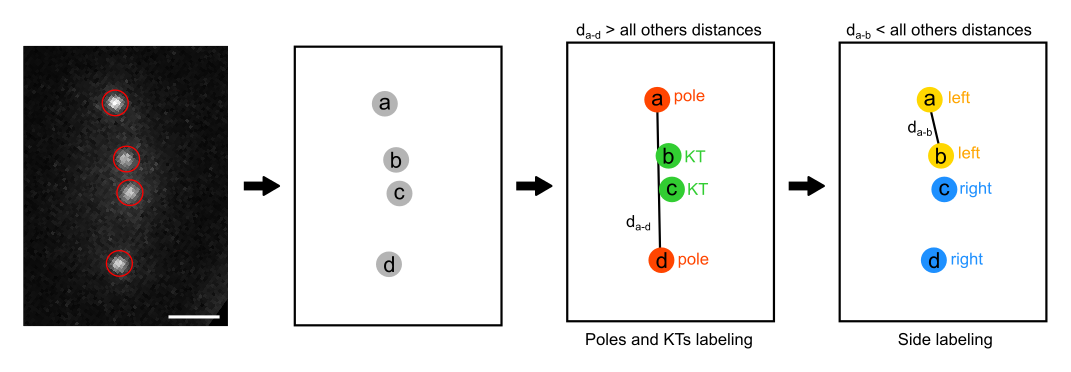
\includegraphics{figures/results/imaging/algo_cen2.png}
\caption[Algorithme de tracking pour un chromosome]{\label{fig:algo_cen2}Algorithme
de tracking pour un chromosome.}
\end{figure}

Cette technique est très robuste (Figure~\ref{fig:cen2}). Cependant il
arrive parfois que quelques erreurs subsistent dans les trajectoires. On
peut alors avoir recours à une interface de correction manuelle des
trajectoires.

\begin{figure}[htbp]
\centering
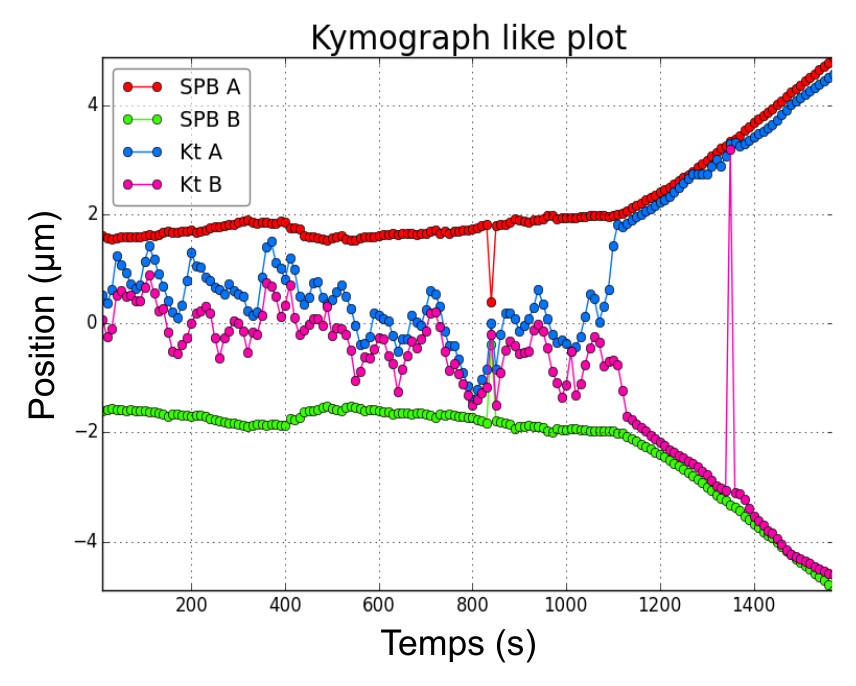
\includegraphics{figures/results/imaging/cen2.png}
\caption[Reconstruction de la trajectoire du chromosome II et de ces deux pôles.]{\label{fig:cen2}Reconstruction
de la trajectoire du chromosome II et de ses deux pôles.}
\end{figure}

\paragraph{Interface de correction manuelle des
trajectoires}\label{interface-de-correction-manuelle-des-trajectoires}

Afin de pouvoir facilement corriger les trajectoires des chromosomes
contenant des erreurs qu'il aurait été dommage d'écarter de l'analyse,
il a été développé une interface graphique de correction manuelle. Cette
interface écrite en Python est basé sur la bibliothèque
\texttt{pyqtgraph}.\footnote{\url{www.pyqtgraph.org}} Son code est
librement disponible.\footnote{\url{http://git.io/vCNxh}}

L'interface permet de naviguer de manière intuitive dans la trajectoire
à l'aide d'un système de zoom dynamique (Figure~\ref{fig:gui}). Il est
possible de visualiser en deux dimensions n'importe quelle information
contenue dans la trajectoire telles que le temps, la position en \(x\),
\(y\) et \(z\) (si disponible), la taille et l'intensité des blobs, etc.
Elle permet aussi d'annoter les trajectoires en leur donnant une note
comprise entre un et trois décrivant la qualité de la trajectoire. Enfin
il est possible de spécifier le début de l'anaphase
(Figure~\ref{fig:gui}A) afin de pouvoir faciliter l'analyse automatique
des différentes phases de la mitose ultérieurement.

Cependant l'utilité majeure de l'interface graphique est de pouvoir
modifier les erreurs de tracking (Figure~\ref{fig:gui}B). Ainsi il est
possible de sélectionner un ou plusieurs blobs en même temps afin de les
supprimer. On peut aussi sélectionner deux trajectoires afin de les
raccorder, de les fusionner ou bien de les séparer.

\begin{figure}[htbp]
\centering
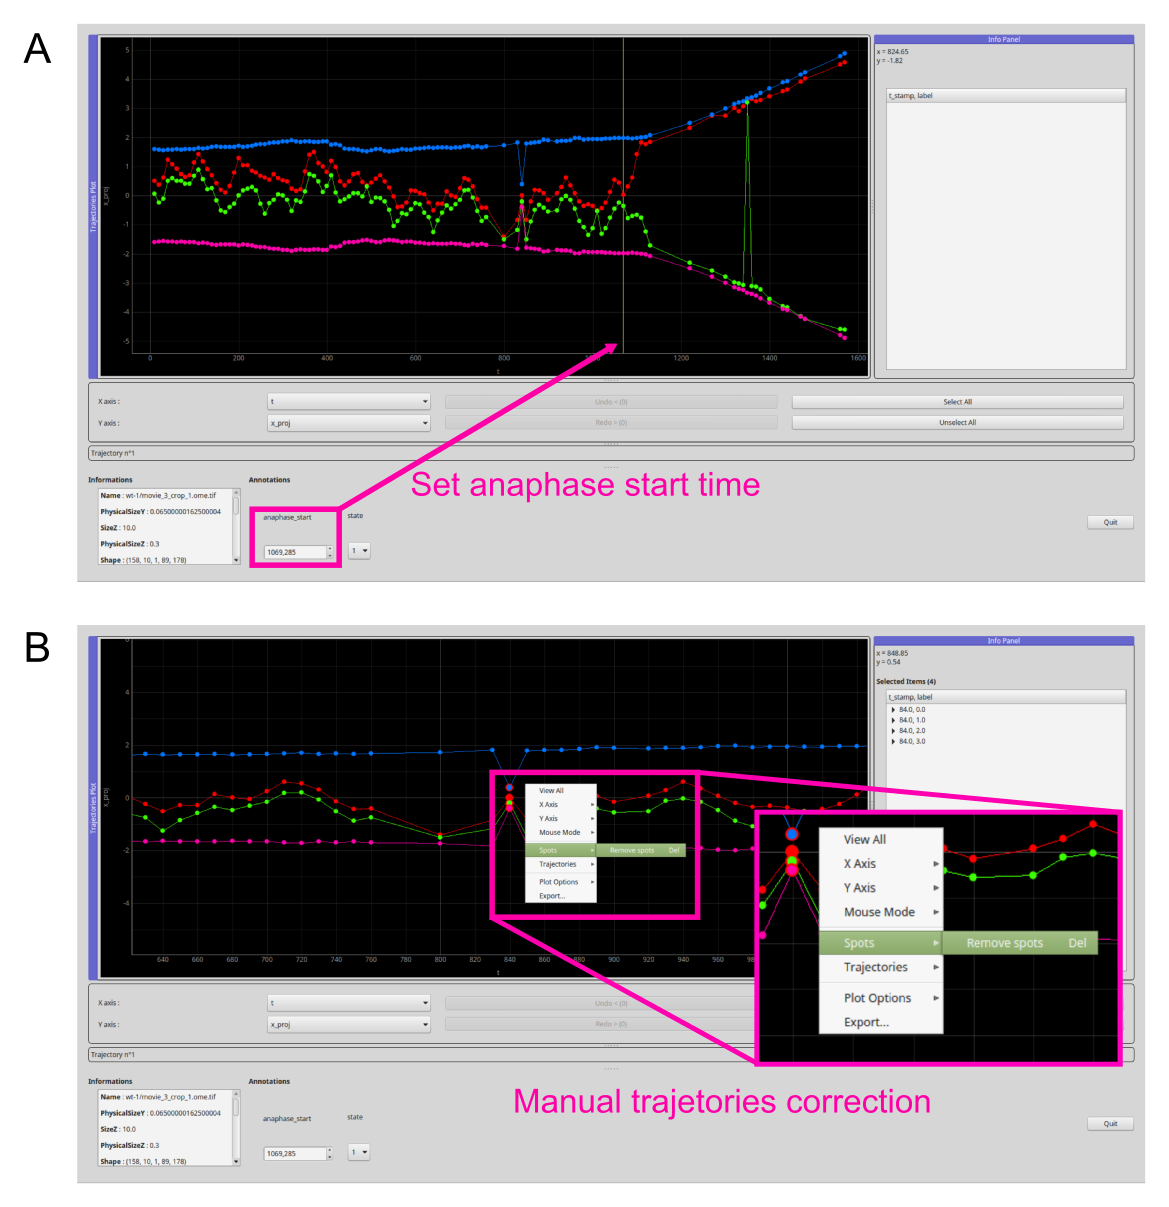
\includegraphics{figures/results/imaging/gui.png}
\caption[Interface graphique de correction manuelle des trajectoires]{\label{fig:gui}Interface
graphique de correction manuelle des trajectoires. \textbf{A}. Le début
de l'anaphase peut être modifier manuellement. \textbf{B}. Chaque
trajectoire peut être modifié à l'aide d'une interface simple et
intuitive.}
\end{figure}

\subsubsection{Résumé du workflow de reconstruction des
trajectoires}\label{ruxe9sumuxe9-du-workflow-de-reconstruction-des-trajectoires}

Voici un résumé de l'ensemble des étapes menant à la reconstruction de
la trajectoire des chromosomes (Figure~\ref{fig:workflow}). En entrée,
on possède un film issu de la vidéo-microscopie à fluorescence contenant
la dynamique des chromosomes et des pôles du fuseau mitotique durant la
mitose. En sortie, on obtient la trajectoires de chacun des objets qui
contient les positions ainsi que les propriétés géométriques des blobs
pour chaque pas de temps.

\begin{figure}[htbp]
\centering
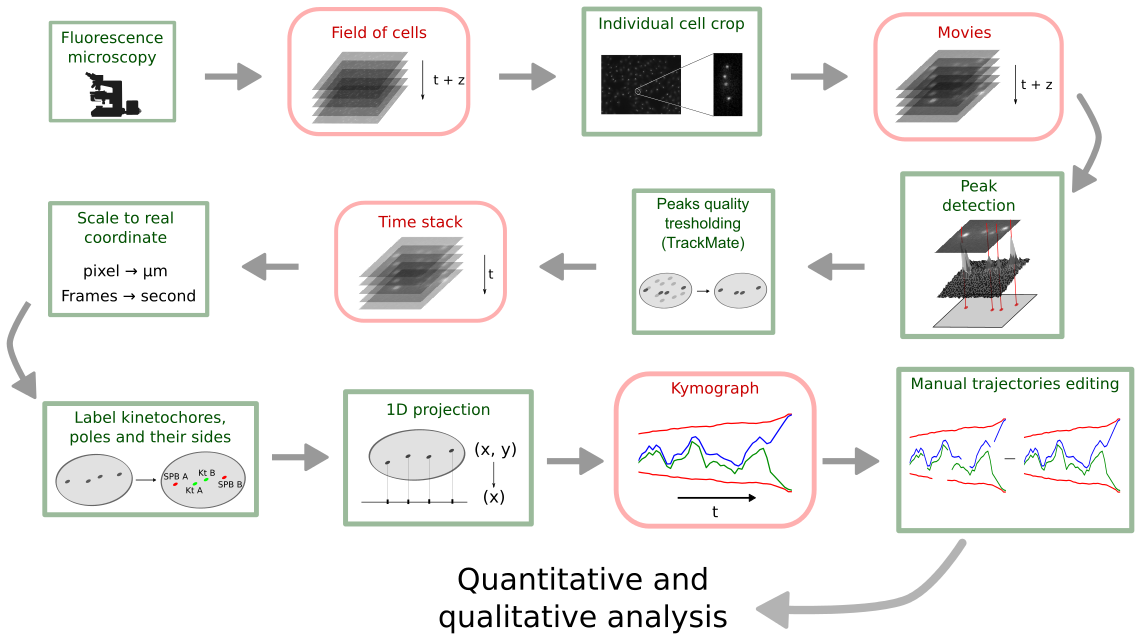
\includegraphics{figures/results/imaging/workflow.png}
\caption[Workflow de reconstruction des trajectoires]{\label{fig:workflow}Workflow
de reconstruction des trajectoires. Deux étapes nécessitent une
intervention manuelle. Suite à la détection de blobs (peaks) et après la
reconstruction automatique des trajectoires.}
\end{figure}

La constitution d'une base de donnée de trajectoires contenant
différentes souches cellulaires permet par la suite de comparer les
différents groupes de trajectoires afin d'en extraire leurs principales
propriétés biophysiques.

\subsection{L'état de cohérence du mouvement des kinétochores
frères}\label{luxe9tat-de-cohuxe9rence-du-mouvement-des-kinuxe9tochores-fruxe8res}

En plus des propriétés oscillatoires telles que l'amplitude ou la
période des mouvements (voir Section~\ref{sec:article} pour les
résultats de cette analyse), il est aussi possible d'analyser la
cohérence du mouvement des kinétochores (Armond et al.
(\hyperref[ref-Armond2015]{2015})).

On définit la cohérence d'un mouvement pour deux kinétochores frères
comme étant l'état de synchronisation du mouvement de chaque kinétochore
en fonction de son kinétochore frère. Par exemple, si un kinétochore a
un mouvement poleward (P), le mouvement du chromosome est cohérent si
son kinétochore frère à un mouvement anti-poleward (AP)
(Figure~\ref{fig:coherence_schema}).

\begin{figure}[htbp]
\centering
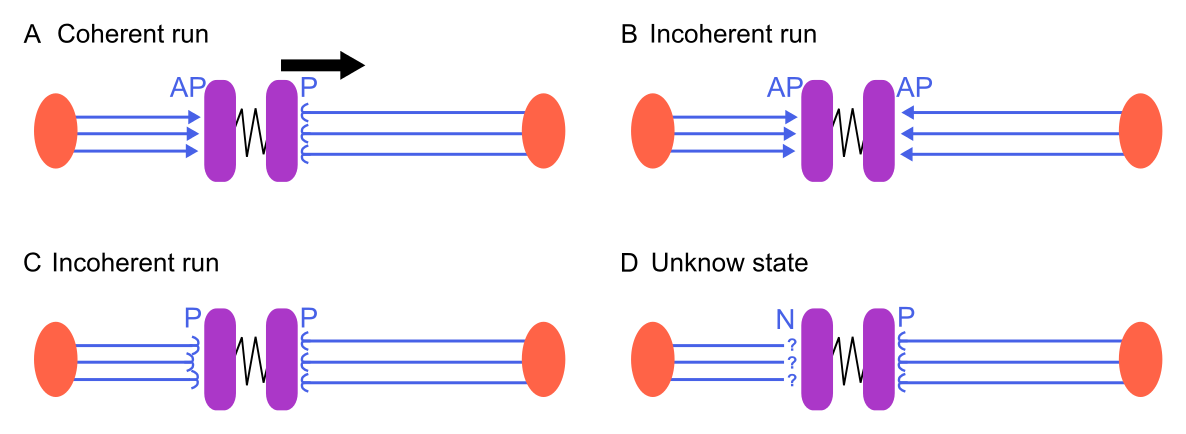
\includegraphics{figures/results/imaging/coherence_schema.png}
\caption[Schéma de mouvement cohérent et incohérent des kinétochores frères.]{\label{fig:coherence_schema}Schéma
de mouvement cohérent et incohérent des kinétochores frères. \textbf{A}.
Les deux kinétochores frères sont dans des états poleward et
anti-poleward, le mouvement est cohérent. \textbf{B} et \textbf{C}. Les
deux kinétochores frères sont dans le même état poleward ou
anti-poleward, le mouvement est incohérent. \textbf{D}. Dans certains
cas il est impossible de déterminer précisément l'état de cohérence d'un
chromosome.}
\end{figure}

La méthode (Armond et al., \hyperref[ref-Armond2015]{2015}) consiste à
assigner une direction (poleward (P), anti-poleward (AP) ou inconnu (N))
à chaque kinétochore indépendamment les uns des autres. La direction
pour un pas de temps est déterminée en regardant le signe du mouvement à
ce temps ainsi que le signe des mouvements autour de ce pas de temps
dans une fenêtre de taille \(w\). On assigne ainsi pour chaque pas de
temps un score qui selon sa valeur classe le pas de temps en P, AP ou N
(Figure~\ref{fig:coherence_schema}).

\[
S_i = \frac{n_p - n_{AP}}{2w - 1}
\]

Où \(n_P\) et \(n_{AP}\) sont le nombre de pas de temps contenant un
état poleward et anti-poleward dans la fenêtre de temps de taille \(w\).
L'état est déterminé en regardant le signe du mouvement en fonction de
la position du pôle. Les pas de temps avec \(S_i < -S*\) sont assignés
comme P. Les pas de temps avec \(S_i > S*\) sont assignés comme AP. Les
paramètres ont été fixé manuellement avec \(S* = 0.15\) et \(w = 10\)
(avec \(dt=100ms\)). Si \(-S* < S_i < S*\) alors le pas de temps est
considéré comme n'ayant pas de direction (N).

Bien que cette méthode soit grandement dépendante de \(S*\), elle reste
efficace pour pouvoir comparer des trajectoires provenant de différentes
conditions.

Dans une cellule sauvage, on observe que le kinetochore est le plus
souvent dans l'état opposé à son kinétochore frère bien qu'il existe de
courtes périodes de temps où les deux kinétochores sont dans un état
incohérent (Figure~\ref{fig:coherence_kymo}, voir le mouvement entre
220s et 230s).

\begin{figure}[htbp]
\centering
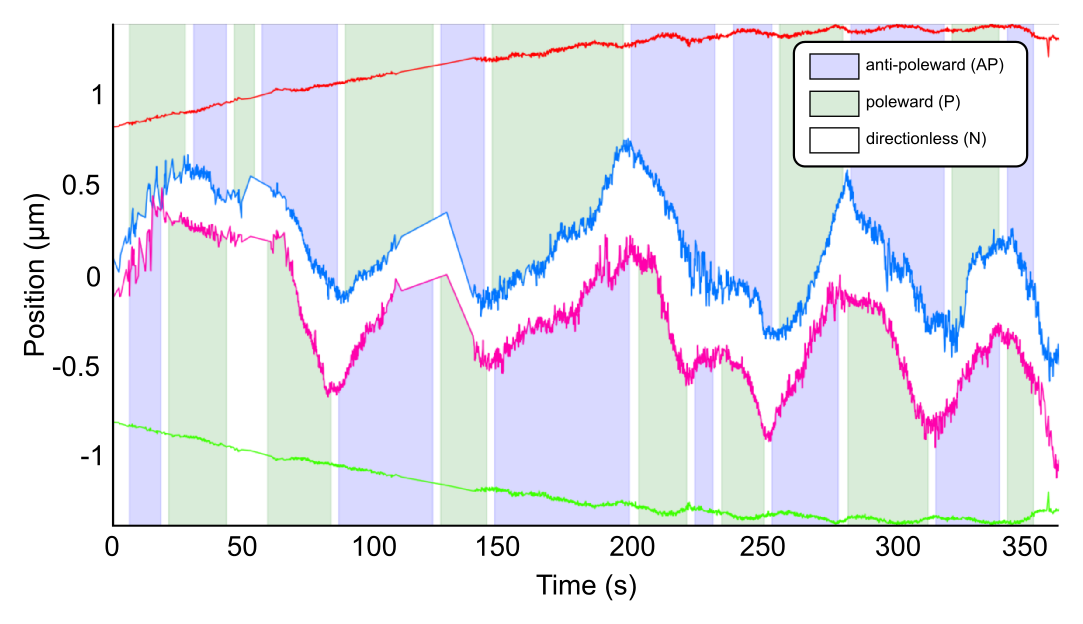
\includegraphics{figures/results/imaging/coherence_kymo.png}
\caption[Direction des kinétochores frères en metaphase.]{\label{fig:coherence_kymo}Direction
des kinétochores frères en metaphase. Trajectoires des pôles (rouge et
vert) et des kinétochores frères (bleu et rose) en métaphase dans une
cellule sauvage. Le pas de temps de l'acquisition est de 100ms.}
\end{figure}

Si l'on compare les états de cohérence de plusieurs cellules dans
différentes conditions (Figure~\ref{fig:coherence-stats}) on observe que
les kinétochores des mutants kinésine-8 (\emph{klp6Δ}, \emph{klp5Δ} et
\emph{klp56Δ}) passent plus de temps dans un état incohérent que dans
les cellules sauvages. Plus précisément, l'état incohérent AP-AP semble
privilégié alors que l'état P-P semble être le même que dans les
cellules sauvages.

\begin{figure}[htbp]
\centering
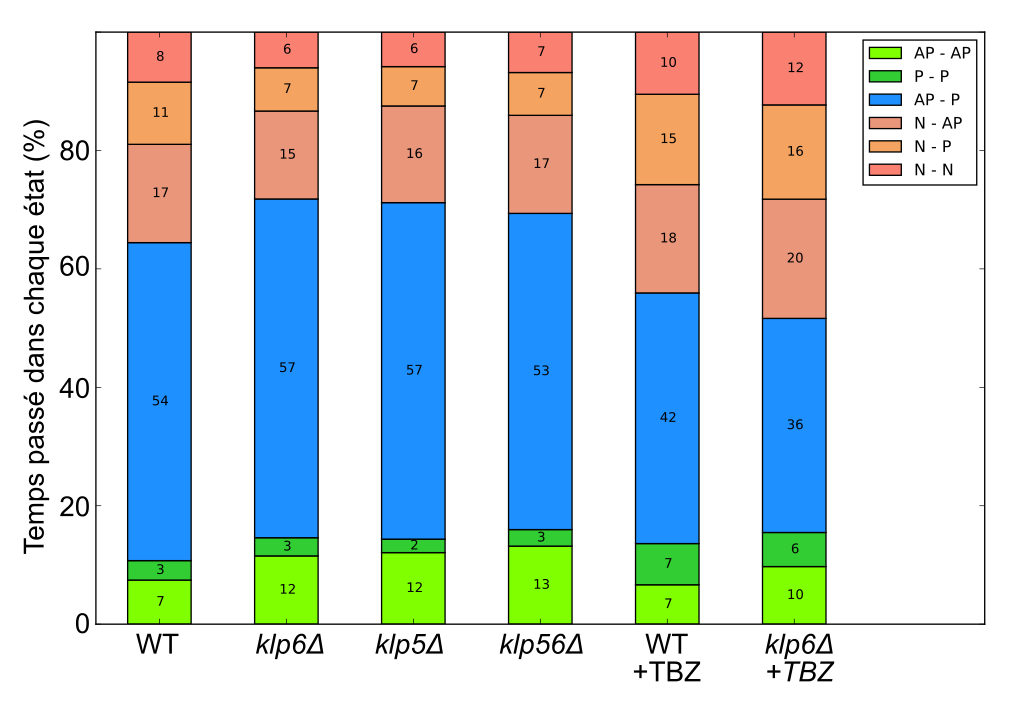
\includegraphics{figures/results/imaging/coherence_stats.png}
\caption[Temps passé dans les différents états de cohérence dans différentes conditions]{\label{fig:coherence-stats}Temps
passé dans les différents états de cohérence dans diverses conditions.
WT désigne une cellule sauvage. \emph{klp6Δ}, \emph{klp5Δ} et
\emph{klp56Δ} désigne différents mutants de la kinésine-8 qui possèdent
tous le même phénotype (voir Section~\ref{sec:article} pour plus de
détails). TBZ désigne une drogue, le thiabendazole qui inhibe les
oscillations des chromosomes en métaphase. Le nombre de cellules
utilisées pour cette analyse est n = 24 pour WT, n = 18 pour
\emph{klp6Δ}, n = 12 pour \emph{klp5Δ}, n = 26 pour \emph{klp56Δ}, n =
19 pour WT+TBZ, n = 14 pour \emph{klp6Δ}+TBZ.}
\end{figure}

Si l'on suppose que le mouvement P implique que les microtubules
associés soient en majorité dans un état de dépolymérisation et que le
mouvement AP implique que les microtubules associés soient en majorité
dans un état de polymérisation (Armond et al.,
\hyperref[ref-Armond2015]{2015}) alors cette observation pourrait
indiquer que la kinésine-8 participe activement à la synchronisation du
mouvement des kinétochores frères.

La distance inter-kinétochore peut être un bon moyen pour quantifier la
tension exercée sur les kinétochores par les microtubules. De cette
façon, en observant la distance inter-kinétochore en fonction de l'état
de cohérence dans différentes conditions, on voit que de manière assez
subtile la distribution des distances pour un état cohérent (AP-P) est
en moyenne de 400nm dans toutes les conditions. Elle semble par ailleurs
très légèrement supérieure pour l'état incohérent P-P et très légèrement
inférieure pour l'état incohérent AP-AP. Bien que ces résultats ne soit
pas significatifs, ils pourraient supporter l'idée qu'un mouvement AP
implique une force de poussée tandis qu'un mouvement P implique une
force de traction sur le kinétochore.

\begin{figure}[htbp]
\centering
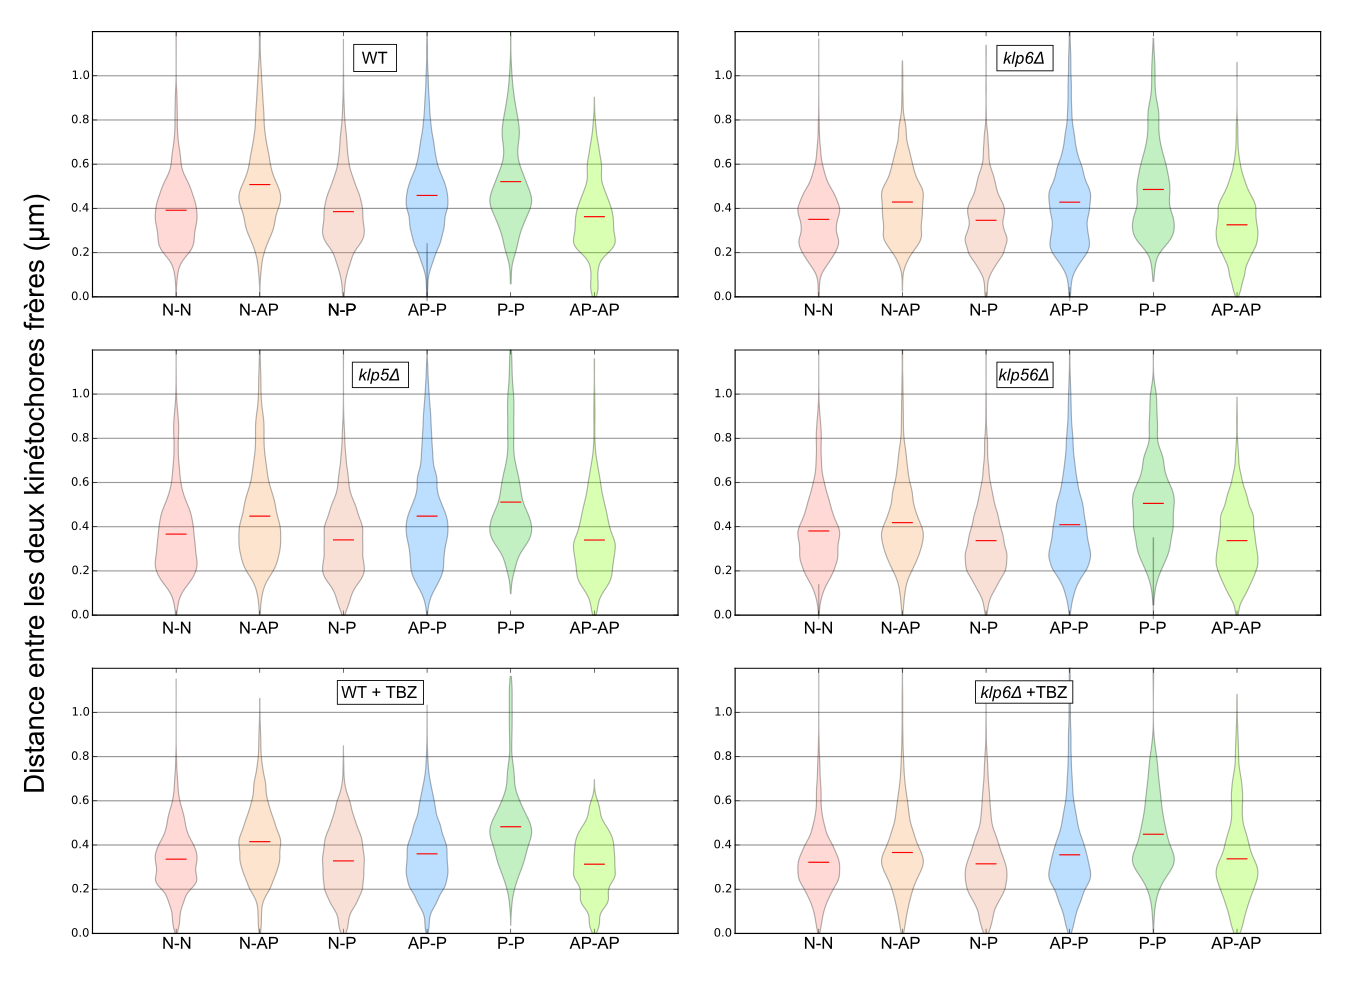
\includegraphics{figures/results/imaging/coherence_stretch.png}
\caption[Distance inter-kinétochore en fonction de l'état de cohérence dans différentes conditions]{\label{fig:coherence_stretch}Distance
inter-kinétochore en fonction de l'état de cohérence dans différentes
conditions. La barre rouge des violin plots désigne la moyenne. WT
désigne une cellule sauvage. \emph{klp6Δ}, \emph{klp5Δ} et \emph{klp56Δ}
désigne différents mutants de la kinésine-8 qui possède tous le même
phénotype (voir Section~\ref{sec:article} pour plus de détails). TBZ
désigne une drogue, le thiabendazole qui inhibe les oscillations des
chromosomes en métaphase. Le nombre de cellule utilisés pour cette
analyse est n = 24 pour WT, n = 18 pour \emph{klp6Δ}, n = 12 pour
\emph{klp5Δ}, n = 26 pour \emph{klp56Δ}, n = 19 pour WT+TBZ, n = 14 pour
\emph{klp6Δ}+TBZ.}
\end{figure}

Cette dernière observation nécessite d'être confirmée car la mesure de
la distance inter-kinétochore dans ce système pourrait comporter un
biais important. En effet, le mutant Cen2-GFP possède une sonde
fluorescente au niveau de la partie péri-centromérique de la chromatide,
donc proche mais pas tout à fait au même endroit que le kinétochore. La
distance entre les deux positions a été estimée à 125nm (Gay et al.,
\hyperref[ref-Gay2012a]{2012}) ce qui est bien plus que la différence
observée. De plus la sonde ne se situe pas dans l'axe des deux
kinétochores frères ce qui signifie qu'une traction ou une poussée sur
cet axe pourrait bien être invisible en mesurant la distance entre les
sonde Cen2-GFP.

Pour finir, on notera quand même que la légère différence de distance
inter-kinétochore pour les états AP-AP et P-P est retrouvée dans toutes
les conditions observées et vont à chaque fois dans le même sens. Cela
constitue tout de même une forte indication que la distance
inter-kinétochore varie de manière significative. Le système Cen2-GFP ne
serait simplement pas assez précis pour capter l'amplitude totale de
cette variation.

L'analyse de l'état de cohérence des kinétochores est une observation
dans des fenêtres de temps relativement grande de l'ordre de 10s. Il est
possible d'analyser les trajectoires dans des fenêtre de temps réduite
d'un facteur 10 à 100 afin de capter les propriétés biophysique sous
jacentes qui contrôlent le mouvement des kinétochores au niveau
moléculaire.

\subsection{Analyse du mouvement par « Mean Square Displacement
»}\label{analyse-du-mouvement-par-mean-square-displacement}

\subsubsection{La MSD, un outil pour accéder aux différents phénomènes
gouvernant un
mouvement}\label{la-msd-un-outil-pour-accuxe9der-aux-diffuxe9rents-phuxe9nomuxe8nes-gouvernant-un-mouvement}

Les mouvements observés au niveau subcellulaire peuvent être dirigés par
des processus différents qu'on peut diviser en trois familles :

\begin{itemize}
\item
  un mouvement purement diffusif (aussi appelé mouvement brownien)
  gouverné par par l'ensemble des chocs de petites particules sur une
  particule plus grosse. Il en résulte un mouvement aléatoire dans
  toutes les dimensions de l'espace.
\item
  un mouvement confiné qui est restreint dans l'espace, par exemple à
  cause d'une paroi cellulaire ou subcellulaire contraignant le
  mouvement d'une protéine. Il est souvent ajouté par dessus un
  mouvement diffusif.
\item
  un mouvement dirigé qui est principalement gouverné par une force
  s'appliquant sur l'objet le mettant ainsi en mouvement dans une
  direction particulière.
\end{itemize}

Dans la réalité les mouvements observés sont souvent dirigés par un
mélange de ces trois processus.

L'outil communément utilisé pour l'étude de ces processus est la mesure
du « Mean Square Displacement » (MSD) qui représente l'étendue spatiale
explorée (caractérisé par une aire dans le cas d'un mouvement en deux
dimensions) en fonction de différents intervalles de temps \(\tau\).

Si on suppose ces processus stationnaires, il est possible de les
modéliser tel que :

\begin{itemize}
\tightlist
\item
  pour un mouvement diffusif (mouvement brownien) :
\end{itemize}

\[
\mbox{MSD}(\tau) = 2dD\tau
\]

Où \(d\) est le nombre de dimensions et \(D\) le coefficient de
diffusion.

\begin{itemize}
\tightlist
\item
  pour un mouvement confiné et diffusif :
\end{itemize}

\[
\mbox{MSD}(\tau) = R_c^2(1-e^{-2dD\tau / R_c})
\]

Où \(R_c\) est la rayon dans lequel la particule est confinée, \(d\) est
le nombre de dimensions et \(D\) le coefficient de diffusion.

\begin{itemize}
\tightlist
\item
  pour un mouvement dirigé :
\end{itemize}

\[
\mbox{MSD}(\tau) = v^2\tau ^2
\]

Où \(v\) est la vitesse de la particule.

On notera par ailleurs qu'il est aussi possible de modéliser une MSD
plus simplement en généralisant simplement le modèle du mouvement
diffusif :

\[
\mbox{MSD}(\tau) = 2dD\tau ^ {\alpha}
\]

Où \(\alpha\) désigne une constante. Si \(\alpha = 1\), on observe un
mouvement diffusif, si \(\alpha > 1\), il s'agit d'un phénomène de
super-diffusion tandis que pour \(\alpha < 1\), le phénomène est appelé
sous-diffusion.

\begin{figure}[htbp]
\centering
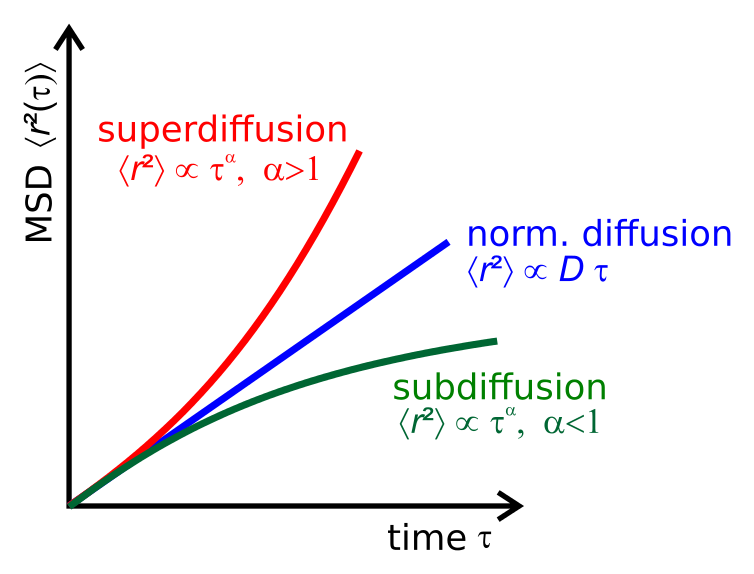
\includegraphics{figures/results/imaging/wiki_diffuse.png}
\caption[Exemple de MSD pour trois types de diffusion théoriques]{\label{fig:wiki_diffuse}Exemple
de MSD pour trois types de diffusion théoriques. Adapté de
https://commons.wikimedia.org/wiki/File\%3AMsd\_anomalous\_diffusion.svg}
\end{figure}

La mesure de la MSD pour une différence de temps \(\Delta t\) est
calculé comme la distance au carré entre la position de l'objet \(r_i\)
au temps \(t\) et sa position au temps \(t+\Delta t\) moyenné sur tout
les temps successifs \(t\) :

\[
\mbox{MSD}(\Delta t) = \langle (r_i(t) - r_i(t + \Delta t)) ^ 2 \rangle
\]

Par exemple, on peut simuler un mouvement brownien et un mouvement
dirigé en deux dimensions (Figure~\ref{fig:motions}A,B). On observe que
dans le cas d'un mouvement brownien, l'aire explorée (la MSD) est
beaucoup plus petite pour un même délai que dans le cas d'un mouvement
dirigé.

\begin{figure}[htbp]
\centering
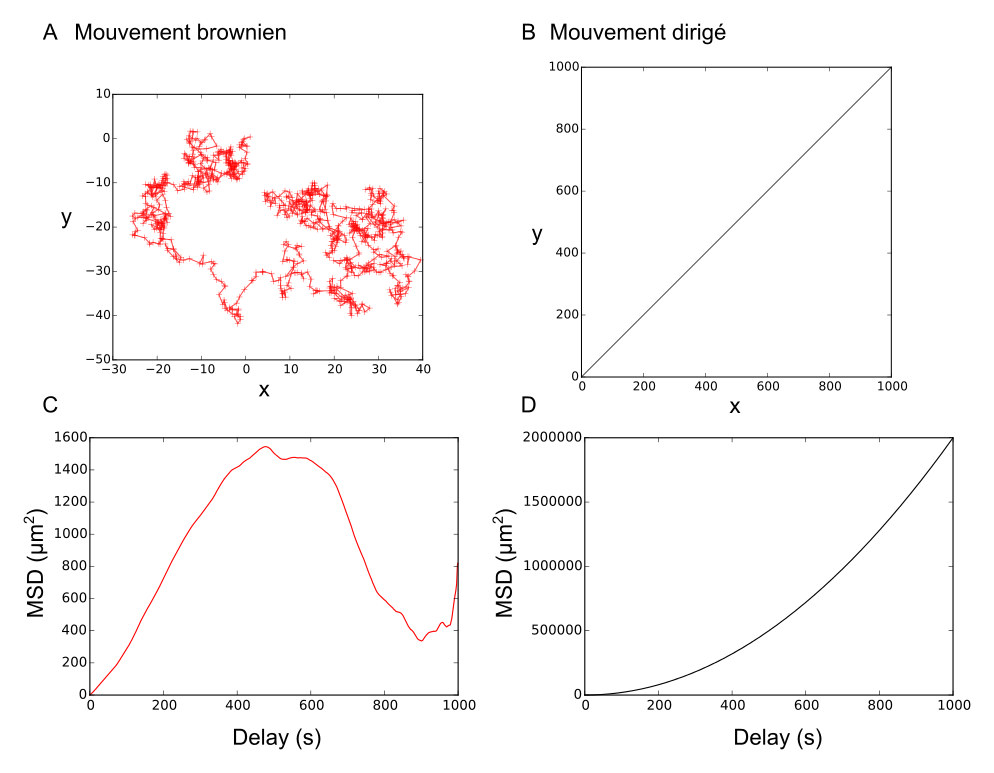
\includegraphics{figures/results/imaging/motions.png}
\caption[Exemple de MSD pour un mouvement dirigé et un mouvement brownien simulé]{\label{fig:motions}Exemple
de MSD pour un mouvement dirigé et un mouvement brownien simulé.
\textbf{A} et \textbf{B}. Évolution des positions d'une particule en
deux dimensions dans le cas d'un mouvement respectivement brownien et
dirigé simulé. \textbf{C} et \textbf{D}. MSD correspondant aux
mouvements en \textbf{A} et \textbf{B}.}
\end{figure}

En fittant des mesures de mouvement de particules avec les équations
décrites précédemment on peut trouver le mouvement majoritaire qui
gouverne le processus (diffusif, dirigé ou confiné) ainsi qu'accéder aux
paramètres physiques gouvernant ces phénomènes tels que le coefficient
de diffusion \(D\), la vitesse de la particule \(v\) ou encore le volume
de confinement \(R_C\).

Cette approche est appelée modélisation basé sur les données («
data-driven modeling » en anglais). Toute la difficulté est de trouver
la bonne technique pour remonter aux équations à partir des données. Un
article publiée par Monier et al. (Monnier et al.,
\hyperref[ref-Monnier2012]{2012}) propose une approche basée sur les
statistiques bayésiennes afin de prédire pour différents types de
mouvement le processus à l'origine ainsi que les paramètres associés.

\subsubsection{Mesure de la MSD appliquée au mouvement de
Cen2-GFP}\label{mesure-de-la-msd-appliquuxe9e-au-mouvement-de-cen2-gfp}

L'observation des MSD de différentes trajectoires de Cen2-GFP sous
différentes conditions (Figure~\ref{fig:msds} et
Figure~\ref{fig:msds-log} pour une visualisation en log-log) fait
apparaître une sur-diffusion des trajectoires dans les cellules délétées
pour la kinésine-8 (\emph{klp6Δ}, \emph{klp5Δ} et \emph{klp56Δ}) ce qui
concorde avec une augmentation de l'amplitude (voir
Section~\ref{sec:article}) ainsi qu'une perturbation de l'état de
cohérence du mouvement des kinétochores frères.

On peut aussi observer que les trajectoires avec TBZ sont très largement
sous diffusives comparées aux trajectoires sans TBZ. Ceci confirme
qu'une force net plus faible est appliquée dans ces conditions dû à un
attachement plus faible des kinétochores aux microtubules. Les
kinétochores seront alors soumis à un confinement forcé du fait des
moindres forces s'exerçant sur elles. Cette observation confirme que
l'attachement est primordial dans la génération de la force au niveau du
kinétochore.

\begin{figure}[htbp]
\centering
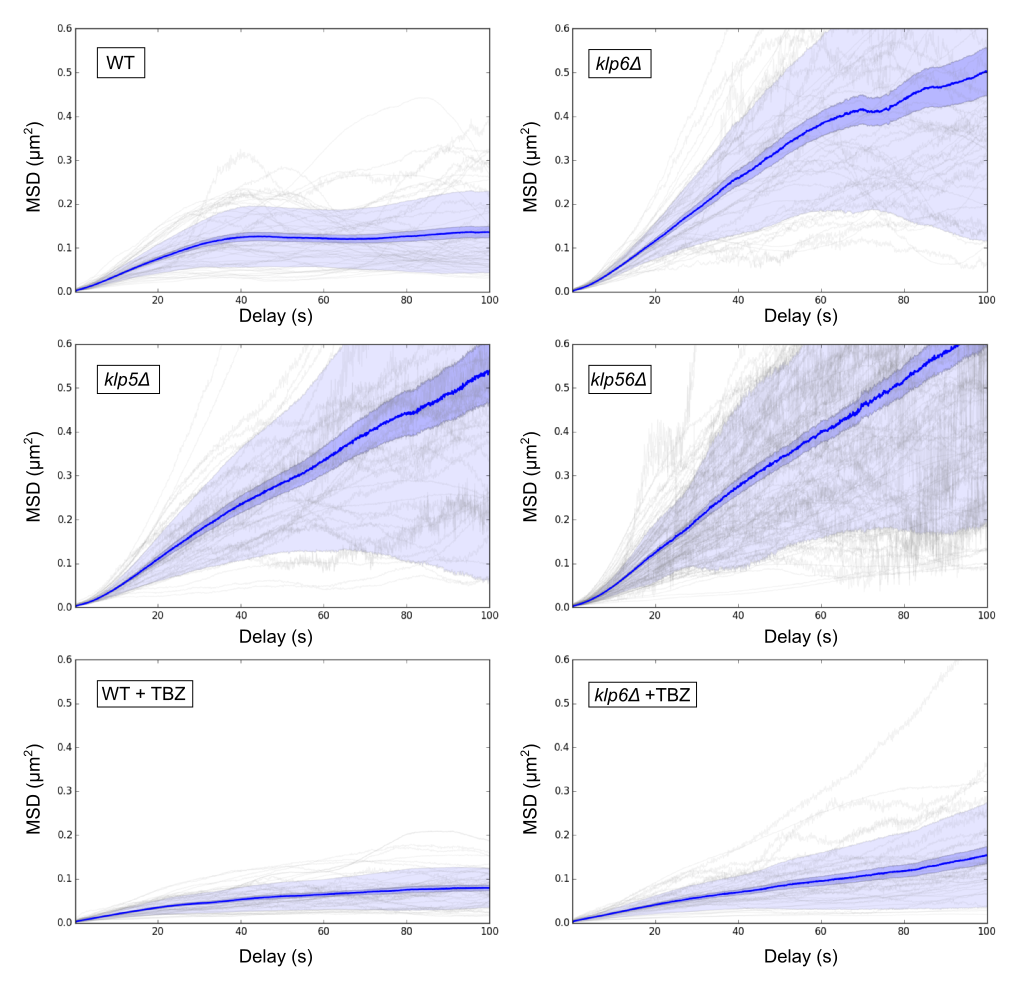
\includegraphics{figures/results/imaging/msds.png}
\caption[MSD pour différentes trajectoires de Cen2-GFP sous différentes conditions.]{\label{fig:msds}MSD
pour différentes trajectoires de Cen2-GFP sous différentes conditions.
La ligne bleu foncé représente la MSD moyenne pondérée par le nombre de
pas de temps pour un délai donné. L'erreur en bleu clair représente
l'erreur standard de la moyenne tandis que l'erreur en bleu très clair
représente la déviation standard. Les MSD en gris correspondent aux MSD
individuelles de chacune des trajectoires. Le nombre de trajectoires
utilisées pour cette analyse est n = 26 pour WT, n = 25 pour
\emph{klp6Δ}, n = 22 pour \emph{klp5Δ}, n = 51 pour \emph{klp56Δ}, n =
23 pour WT+TBZ, n = 19 pour \emph{klp6Δ}+TBZ.}
\end{figure}

La visualisation en log-log (Figure~\ref{fig:msds-log}) permet de voir
de manière plus précise ce qui se passe aux temps courts. Il est ainsi
possible d'observer que toutes les MSD pourraient posséder trois temps
caractéristiques (Figure~\ref{fig:msds-log-fit}) :

\begin{itemize}
\item
  Un premier temps allant juqu'à 0.3s (en orange) pourrait traduire
  l'effet des différents processus aléatoires sur le mouvement
  (mouvement brownien, bruit blanc de la mesure, etc).
\item
  De 0.3s à 2s (en vert), la pente chute brusquement
  (Figure~\ref{fig:msds-log-fit}), ce qui pourrait être la signature de
  la mesure de Cen2-GFP qui bougerait de la même manière qu'une
  particule confinée dû à son éloignement au point où s'exerce les
  forces au niveau du kinétochore et à l'état faiblement rigide de la
  chromatide.
\item
  De 2s à 40s (en bleu), la pente augmente
  (Figure~\ref{fig:msds-log-fit}), ce qui pourrait traduire l'effet dû à
  la force appliquée au niveau des kinétochores. Cette pente serait
  alors caractéristique d'un mouvement dirigé.
\end{itemize}

\begin{figure}[htbp]
\centering
\includegraphics{figures/results/imaging/msds_log.png}
\caption[MSD en log-log pour différentes trajectoires de Cen2-GFP sous différentes conditions]{\label{fig:msds-log}MSD
en log-log pour différentes trajectoires de Cen2-GFP sous différentes
conditions. L'erreur en bleu clair représente l'erreur standard de la
moyenne tandis que l'erreur en bleu très clair représente la déviation
standard. Les MSD en gris correspondent aux MSD individuelles de chacune
des trajectoires. Le nombre de trajectoires utilisées pour cette analyse
est n = 26 pour WT, n = 25 pour \emph{klp6Δ}, n = 22 pour \emph{klp5Δ},
n = 51 pour \emph{klp56Δ}, n = 23 pour WT+TBZ, n = 19 pour
\emph{klp6Δ}+TBZ.}
\end{figure}

Il est d'ailleurs intéressant de remarquer que dans les MSD avec TBZ, la
troisième pente (de 2s à 40s) est plus faible comparée aux MSD sans TBZ.
Cela pourrait signifier que les kinétochores en présence de TBZ sont
soumis des forces plus faibles probablement à cause de l'effet du TBZ
sur la dynamique des microtubules. Cela souligne le rôle capital des
microtubules dans la génération de la force au niveau des kinétochores.
On note aussi que cette observation est confirmé par l'analyse des
oscillations (Mary et al., \hyperref[ref-Mary2015]{2015}). Pour
confirmer ce résultat il faudrait mesurer cette troisième pente en
faisant varier les concentrations de TBZ et regarder si une corrélation
existe.

\begin{figure}[htbp]
\centering
\includegraphics{figures/results/imaging/msds_log_fit.png}
\caption[Régression linéaire sur des MSD pour différentes trajectoires de Cen2-GFP sous différentes conditions]{\label{fig:msds-log-fit}Régression
linéaire sur des MSD pour différentes trajectoires de Cen2-GFP sous
différentes conditions. La régression linéaire a été faite en utilisant
la fonction \texttt{scipy.stats.linregress} de la bibliothèque python
\texttt{scipy}. Les temps choisis pour les trois différentes régressions
sont : de 0.1s à 0.3s, de 0.3s à 2s et de 2s à 40s.}
\end{figure}

Des analyses plus précises sont nécessaires pour pouvoir conclure sur
les différents types de phénomènes mis en jeu dans le mouvement des
chromosomes. Il serait notamment intéressant de comparer le mouvement de
Ndc80-GFP (situé au niveau du kinétochore) avec celui de Cen2-GFP.

Il pourrait être par la suite utile de modéliser à partir de ces
différentes mesures les modèles de mouvement vus dans la section
précédente. L'approche bayésienne semble être une approche intéressante
dans ce type de problème (Monnier et al.,
\hyperref[ref-Monnier2012]{2012}).

\section{Modélisation bio-mécanique de la ségrégation des
chromosomes}\label{moduxe9lisation-bio-muxe9canique-de-la-suxe9gruxe9gation-des-chromosomes}

La modélisation \emph{in silico} des trajectoires des chromosomes en
mitose permet de mieux comprendre quel sont les mécanismes sous-jacent
responsables de la régulation de ces mouvements. L'approche « modèles de
connaissance », qui s'inspire de la mécanique du point, est utilisé et
permet d'établir des hypothèses sur les mécanismes de congression des
chromosomes en métaphase. Enfin d'autre hypothèses sont aussi envisagées
afin de décrire les oscillations du mouvement des chromosomes observées
\emph{in vivo}.

\subsection{\texorpdfstring{\texttt{kt\_simul} : l'implémentation
numérique du modèle de ségrégation des
chromosomes}{kt\_simul : l'implémentation numérique du modèle de ségrégation des chromosomes}}\label{ktux5fsimul-limpluxe9mentation-numuxe9rique-du-moduxe8le-de-suxe9gruxe9gation-des-chromosomes}

L'implémentation numérique du modèle (appelée \texttt{kt\_simul})
précédemment développé par Tournier et al. (Gay et al.,
\hyperref[ref-Gay2012a]{2012}) est disponible en libre accès sous
licence open-source à cette adresse :
\texttt{https://github.com/bnoi/kt\_simul}. Le code source est basé sur
le langage de programmation Python ainsi que l'ensemble des librairies
scientifique associées (« Scipy », Oliphant
(\hyperref[ref-Oliphant2007]{2007})).

Dans le but de rendre \texttt{kt\_simul} plus facilement utilisable et
modifiable, une partie du travail a consisté à refactoriser le code
pré-existant. Il est ainsi possible d'exécuter une simulation en une
dizaine de ligne de codes. Différentes options sont disponibles pour
récupérer ou visualiser les données générées par la simulation. Pour un
exemple d'utilisation voir l'annexe en Section~\ref{sec:ktsimul}.

L'exécution d'un grand nombre de simulations peut prendre du temps,
c'est pour cela qu'a été aussi ajouté à \texttt{kt\_simul}, des
fonctions permettant la répartition de différentes simulations sur
différents cœurs de la machine qui les exécute
(Figure~\ref{fig:parallel}). La parallélisation permet une réduction
drastique des temps de calcul sans avoir à requérir à un puissant
cluster, souvent cher et difficile d'accès. Ainsi une station de travail
classique, équipé de 16 cœurs Intel Xeon E5-2650 cadencé à 2GHz, est
capable d'exécuter plus de 2000 simulations standards en une heure
tandis que la version non parallélisée en exécute seulement 200.

\begin{figure}[htbp]
\centering
\includegraphics{figures/results/modelling/parallel.png}
\caption[Schéma décrivant le principe de la parallélisation en informatique]{\label{fig:parallel}Schéma
décrivant le principe de la parallélisation en informatique. Différence
de vitesse d'exécution théorique entre une implémentation parallélisée
et une implémentation séquentielle. Un algorithme parallélisé (en bleu)
utilise les différents cœurs de la machine pour exécuter plusieurs
simulations en même temps. Donc une machine possédant deux cœurs exécute
en théorie les quatre simulations deux fois plus vite qu'un algorithme
non parallélisé (en rose).}
\end{figure}

\texttt{kt\_simul} permet donc de modifier le modèle facilement. Il a
été utilisé pour tester plusieurs hypothèses afin de mieux comprendre
l'alignement et le mouvement des chromosomes.

\subsection{Un modèle de congression
alternatif}\label{un-moduxe8le-de-congression-alternatif}

L'étude publiée dans le cadre de ce travail de thèse (Mary et al.,
\hyperref[ref-Mary2015]{2015}) a montré que la kinésine-8 pouvait agir
comme un régulateur des forces appliquées sur les kinétochores en
fonction de la position le long du fuseau mitotique.

Il a par ailleurs été montré \emph{in silico} qu'une force dépendante de
la distance au pôle sur le kinétochore pouvait reproduire l'alignement
des chromosomes \emph{in vivo} (Figure~\ref{fig:hyp1} et
Figure~\ref{fig:ch-alignment}) en adaptant un modèle existant de la
congression des chromosomes (Gay et al., \hyperref[ref-Gay2012a]{2012}).
Cette force dépendante de la longueur est gouvernée par un seul
paramètre \(L_{dep}\) qui caractérise l'amplitude de la dépendance en
longueur de cette force. Elle a été optimisée afin de reproduire les
distributions d'alignement \emph{in vivo} (pour le détail de
l'implémentation, se référer aux méthodes de l'article en
Section~\ref{sec:article}, (Mary et al.,
\hyperref[ref-Mary2015]{2015})).

\begin{figure}[htbp]
\centering
\includegraphics{figures/results/modelling/hyp1.png}
\caption[Premier mécanisme expliquant l'alignement des chromosomes]{\label{fig:hyp1}Schémas
et exemple de trajectoire \emph{in silico} du mécanisme d'alignement
avec et sans force dépendante de la longueur.}
\end{figure}

\begin{figure}[htbp]
\centering
\includegraphics{figures/results/modelling/ch_alignment.png}
\caption[Distribution de l'alignement relatif des chromosomes en anaphase]{\label{fig:ch-alignment}Distribution
de l'alignement relatif des chromosomes en anaphase \emph{in vivo} (dans
les cellules WT, n=52 et klp6Δ, n=63) et \emph{in silico} pour
l'hypothèse 1 (avec, n=60 ou sans la force dépendante de la longueur,
n=60) et \emph{in silico} pour l'hypothèse 2 (avec, n=60 ou sans la
force dépendante de la longueur, n=60). Une distance proche de 0
signifie que le chromosome est positionnée au milieu du fuseau
mitotique.}
\end{figure}

L'hypothèse 1, présentée dans ce travail (Section~\ref{sec:article}),
est principalement basée sur des observations \emph{in vivo} et \emph{in
vitro} montrant que la kinésine-8 s'accumule de manière plus importante
au pôle plus du microtubule (Tischer et al.,
\hyperref[ref-Tischer2009]{2009}; Varga et al.,
\hyperref[ref-Varga2006]{2006}, \hyperref[ref-Varga2009]{2009}). Ce
gradient de concentration de kinésine-8 viendrait alors modifier la
dynamique du microtubule kinétochorien. Si les études effectuées dans
différents organismes (cellule humaines, levure à fission et levure à
bourgeon) ne s'accordent pas sur le paramètre exact de la dynamique des
microtubules qui est modifié par la kinésine-8, toutes s'accordent à
dire que la kinésine-8 possède une activité dépolymérisatrice et régule
la longueur des microtubules (Messin and Millar,
\hyperref[ref-Messin2014]{2014}; Walczak et al.,
\hyperref[ref-Walczak2013a]{2013}).

La force dépendante de la longueur, décrite par l'hypothèse 1, peut donc
s'expliquer par le fait que si un microtubule possède une densité plus
élevée de kinésine-8 à une extrémité, il produira une force de traction
plus élevée sur le kinétochore. Bien que cette hypothèse reproduise de
manière fidèle l'alignement ainsi que l'absence de chromosomes
retardataires en anaphase (Figure~\ref{fig:ch-alignment} et aussi Figure
7 de l'article en Section~\ref{sec:article}), le mécanisme proposé est
encore très phénoménologique et le lien entre force de traction et
kinésine-8 reste largement hypothétique.

La flexibilité de l'implémentation du modèle \texttt{kt\_simul} permet
de proposer une hypothèse alternative moins phénoménologique.

L'hypothèse 2 est basé sur l'observation faite que la kinésine-8 peut
contrôler la taille des microtubules (Varga et al.,
\hyperref[ref-Varga2006]{2006}). On peut donc supposer que la
distribution des extrémités plus des microtubules au sein du fuseau
mitotique n'est pas uniforme mais suit une distribution de type «
distribution en cloche » (possédant un paramètre de position et un
paramètre d'échelle) comme une distribution gaussienne par exemple.

L'hypothèse 2 est donc construite sur l'idée que la probabilité
d'attachement va dépendre de la densité d'extrémités plus des
microtubules le long du fuseau. Donc la probabilité d'attachement
devrait varier en fonction de cette distribution de taille des
microtubules.

L'implémentation est basée sur la modification de la probabilité
d'attachement des microtubules aux kinétochores. Dans le modèle initial
(Gay et al., \hyperref[ref-Gay2012a]{2012}), l'attachement est gouverné
de manière stochastique par une une probabilité \(P_{\alpha}\) définie
comme suit :

\[
P_{\alpha} = 1 - e^{k_{\alpha}*dt}
\]

Où \(k_{\alpha}\) est le taux d'attachement et \(dt\) le pas de temps de
la simulation.

Pour modéliser une probabilité d'attachement non uniforme, on modifie le
taux d'attachement \(k_{\alpha}\) en fonction de la position du
kinétochore le long du fuseau mitotique avec un préfacteur \(n_{dep}\)
comme suit :

\[
P_{\alpha} = 1 - e^{k_{\alpha}*dt*n_{dep}(d_{KT})}
\]

Où \(d_{KT}\) représente la distance entre le kinétochore et le pôle
auquel il est attaché (c'est à dire la taille du microtubule).

Puisque nous n'avons pas accès à la distribution des extrémités des
microtubules au sein du fuseau, une distribution suivant une loi de
Cauchy a été choisi (Figure~\ref{fig:hyp2}). Ce type de distribution est
préféré par rapport à une distribution gaussienne plus classique à cause
de sa longue queue qui permet de ne pas interdire les attachements
proches des pôles. On définit \(n_{dep}(d_{KT})\) comme suit :

\[
n_{dep}(d_{KT}) = \dfrac{1}{\pi * \gamma * (\dfrac{d_{KT} - x_0}{\gamma})^2}
\]

Où \(\gamma\) est le paramètre d'échelle (correspondant à la largeur de
la distribution) et \(x_0\) le paramètre de position qui représente la
longueur médiane du microtubule. Afin de garder une valeure moyenne de
\(n_{dep}(d_{KT})\) proche de 1, on normalise le préfacteur \(n_{dep}\)
par la valeur moyenne de la distribution calculée le long du fuseau
mitotique.

L'implémentation de ce modèle (Figure~\ref{fig:hyp2}) permet d'observer
que cette hypothèse est aussi capable de reproduire l'alignement des
chromosomes en mitose (Figure~\ref{fig:ch-alignment}).

\begin{figure}[htbp]
\centering
\includegraphics{figures/results/modelling/hyp2.png}
\caption[Second mécanisme expliquant l'alignement des chromosomes]{\label{fig:hyp2}Schémas
et exemple de trajectoire \emph{in silico} du mécanisme d'alignement
avec et sans taux d'attachement dépendant de la longueur.}
\end{figure}

Aucun du modèle initial (Gay et al., \hyperref[ref-Gay2012a]{2012}) ou
bien des deux hypothèses développées ici ne sont cependant suffisantes
pour reproduire l'amplitude des oscillation des chromosomes observées de
la prométaphase à la métaphase (Jaqaman et al.,
\hyperref[ref-Jaqaman2010]{2010}; Skibbens et al.,
\hyperref[ref-Skibbens1993]{1993}). Il semblerait donc qu'un autre
mécanisme soit requis pour expliquer ce type de mouvement.

Cependant, ni le modèle initial (Gay et al.,
\hyperref[ref-Gay2012a]{2012}) ou les modèles avancés ici ne permettent
de reproduire précisément les mouvements oscillatoires des kinétochores
frères observés de la prométaphase à la métaphase (Jaqaman et al.,
\hyperref[ref-Jaqaman2010]{2010}; Skibbens et al.,
\hyperref[ref-Skibbens1993]{1993}). Comme illustré par la Biologie, il
semble donc que de multiples mécanismes participent aux mouvements
coordonnés des chromosomes en mitose.

\subsection{Vers un modèle d'attachement à trois
états}\label{vers-un-moduxe8le-dattachement-uxe0-trois-uxe9tats}

TODO: LA GUILLAUME SI T'AS DES IDÉES PR RAJOUTER DES TRUCS, N'HESITE
PAS. EN MEME TEMPS ON A EU PEU DE RESULTATS AVEC CA DC BON\ldots{} APRES
JE RESTE CONVAINCU QUE CETTE STRATEGIE EN Y PASSANT UN PEU DE TEMPS PEU
DONNER DES TRUCS SYMPA SANS AVOIR A SORTIR L'ARTILLERIE LOURDE EN
MODELISANT LES MICROTUBULES ET NDC80 COMPLETEMENT.

L'instabilité directionnelle des chromosomes \emph{in vivo} n'est pas
reproduite par le modèle de force balance présenté jusqu'ici. En effet,
les oscillations pourraient requérir un mécanisme encore mal compris
afin de synchroniser les deux kinétochores frères et produire ce type de
mouvement coordonné (Wan et al., \hyperref[ref-Wan2012]{2012}).

On rappelle que le modèle initialement développé par Tournier et al. ne
contient pas de structure pouvant s'apparenter aux microtubules \emph{in
vivo}. En effet, le système est composé d'un attachement à deux états,
qui peut être; soit « ON » et produire une force en direction du pôle,
soit « OFF » et ne produire aucune force (Figure~\ref{fig:two_states}).
Le passage entre les deux états se fait de manière stochastique avec en
plus deux mécanismes de corrections qui peuvent modifier les constantes
d'attachement et de détachement (voir Gay et al.
(\hyperref[ref-Gay2012a]{2012}) pour le fonctionnement de ces deux
mécanismes de corrections).

\begin{figure}[htbp]
\centering
\includegraphics{figures/results/modelling/two_states.png}
\caption[Modèle d'attachement à deux états]{\label{fig:two_states}Modèle
d'attachement à deux états. Le passage d'un état à l'autre se fait de
manière stochastique et est régulé par deux mécanismes de corrections
gouvernés par les deux paramètres \(\beta\) et \(d_\alpha\) (Gay et al.,
\hyperref[ref-Gay2012a]{2012}).}
\end{figure}

Les mouvements des chromosomes dans le modèle sont donc produits par le
passage stochastique d'un état à l'autre. L'idée du modèle d'attachement
à trois états est d'ajouter un niveau de flexibilité supplémentaire dans
la dynamique des attachements et donc aussi dans la dynamique des forces
appliquées aux chromosomes dans le but de produire des mouvements
oscillatoires représentatifs de ceux observés \emph{in vivo}.

L'ajout d'un état permettrait au système de mieux « imiter » l'action
des microtubules sur la dynamique des attachements sans réellement avoir
à modéliser la dynamique des microtubules.

Le concept que les microtubules peuvent « pousser » par polymérisation
et « tirer » par dépolymérisation a été proposé dans les années 70 par
Inoué et Sato (Inoué and Sato, \hyperref[ref-Inoue1967]{1967}). Les
mécanismes gouvernant la production de ces forces devinrent évidentes
lorsque l'instabilité dynamique des microtubules fût découverte
(Mitchison and Kirschner, \hyperref[ref-Mitchison1984]{1984}).

Un des mécanismes possible générant la force de poussée (« pushing force
» en anglais) serait le cliquet brownien (« brownian ratchet » en
anglais) dans lequel les fluctuations thermiques permettrait l'ajout de
dimères de tubuline à l'extrémité plus des microtubules (Peskin et al.,
\hyperref[ref-Peskin1993]{1993}). Par ailleurs, bien que les forces de
poussées ont été observées \emph{in vivo} (Skibbens et al.,
\hyperref[ref-Skibbens1993]{1993}), il est supposé que leur contribution
aux mouvements des chromosomes soient très minoritaires (Khodjakov and
Rieder, \hyperref[ref-Khodjakov1996]{1996}; Waters et al.,
\hyperref[ref-Waters1996a]{1996}) et que la force de traction soit
l'acteur majeur gouvernant le mouvement des chromosomes (Inoué and
Salmon, \hyperref[ref-Inoue1995]{1995}).

Le modèle à trois états propose d'intégrer ces observations
(Figure~\ref{fig:three_states}) :

\begin{itemize}
\item
  L'état « détaché » (D) correspond à un site d'attachement sans
  microtubule et donc sans génération de force.
\item
  L'état « attaché \& dépolymérisant » (SA) correspond à un attachement
  par un microtubule qui génère une force notamment du fait de la
  dépolymérisation du microtubule.
\item
  L'état « attaché \& polymérisant » (GA) correspond à un attachement
  par un microtubule qui polymérise est donc sans production de force.
  L'absence de force est motivé par la faible contribution des forces de
  poussées au mouvement des chromosomes.
\end{itemize}

\begin{figure}[htbp]
\centering
\includegraphics{figures/results/modelling/three_states.png}
\caption[Modèle d'attachement à trois états]{\label{fig:three_states}Modèle
d'attachement à trois états. Les trois états prennent en compte les
différentes observations faites entre la génération de la force au
niveau du kinétochore et la dynamique des microtubules.}
\end{figure}

L'implémentation de ce modèle suppose donc que le passage de D à GA (et
inversement) et de D à SA (et inversement) sont toujours dirigés par les
deux mécanismes déjà décrits dans Gay et al.
(\hyperref[ref-Gay2012a]{2012}) et dépendant des mécanismes de
correction des attachements \(\beta\) et \(d_{\alpha}\).

De plus, il est proposé que le passage de GA à SA soit gouverné par le
taux de catastrophe, \(k_{catastrophe}\), (passage d'un état de
polymérisation à un état de dépolymérisation) du microtubule attaché et
que le passage de SA à GA soit gouverné par le taux de rescue,
\(k_{rescue}\), (passage d'un état de dépolymérisation à un état de
polymérisation) du microtubule attaché (Figure~\ref{fig:three_states}).

Cette implémentation du modèle d'attachements à trois états ajoute donc
deux paramètres mais aucune synchronisation entre les kinétochores
frères. On suppose donc que la présence d'oscillations serait une
caractéristique émergente du système (théorie du kinétochore bête, voir
Khodjakov et al. (\hyperref[ref-Khodjakov1999]{1999})).

Un modèle plus complexe serait de moduler \(k_{rescue}\) et
\(k_{catastrophe}\) en fonction de la vitesse de déplacement du
kinétochore, qui correspond à la vitesse de polymérisation et
dépolymérisation du microtubule attaché.

Ainsi le système introduit un mécanisme de communication entre les deux
kinétochores frères et on suppose alors que les oscillations proviennent
directement de la capacité des kinétochores à détecter l'état dans
lequel ils sont (théorie du kinétochore intelligent, voir Khodjakov et
al. (\hyperref[ref-Khodjakov1999]{1999})).

Un exemple d'implémentation de la modulation des taux de catastrophe et
de rescue pourrait prendre cette forme :

\[
k_{rescue} = \frac{kmax_{rescue}}{1 + e^{\frac{-v}{v_{shrink}}}}
\]

\[
k_{catastrophe} = \frac{kmax_{catastrophe}}{1 + e^{\frac{-v}{v_{growth}}}}
\]

GUILLAUME: JAI DU MAL A ME SOUVENIR/COMPRENDRE PK ON A CONSTRUIT UNE
MODULATION BASE SUR DES VITESSE. NE POURRAIT ON PAS FAIRE UN SWITCH
DEPENDANT DE LA TENSION DONC DU STRETCH (SI ON SUPPOSE UN COEF DE
RAIDEUR CONSTANT) COMME PROPOSE DANS LES MODELES STANDARD (VOIR Rieder
and Salmon, 1994 ET PLUS RECEMMENT
http://elifesciences.org/lookup/doi/10.7554/eLife.09500) ??? (par contre
pas le temps de tester, je peux en parler en discussion)

GUILLAUME: JE VIENS DE FINIR
http://elifesciences.org/lookup/doi/10.7554/eLife.09500 ET EN FAITE ILS
DISENT QUE AU CONTRAIRE LE SWITCH PEUT PAS SEXPLIQUER PAR JUSTE UN
TRESHOLD SUR LA TENSION SINON ON POURRAIT JAMAIS AVOIR DES OSCILLATIONS
AUSSI NET (VOIR LA FIGURE 4A DE L'ARTICLE ELIFE POUR LES DETAILS). DU
COUP IL PROPOSE UN ``switching time regulator'' (A TENSION CLOCK MODEL),
VOIR FIGURE 6).

Où \(v_{growth}\) et \(v_{shrink}\) serait les vitesses maximales de
polymérisation de dépolymérisation des microtubules attachés au
kinétochore.

Ici on rajoute donc quatre paramètres libres (\(kmax_{rescue}\),
\(kmax_{catastrophe}\), \(v_{growth}\) et \(v_{shrink}\)) en plus des
deux autres déjà présent (\(\beta\) et \(d_{\alpha}\)).

La dynamique globale de l'attachement ayant changé, il est nécessaire de
recalculer la force de calage de la zone interdigitée (\(F_{mz}\)) afin
de garder un fuseau en équilibre de force et un taux d'élongation du
fuseau mitotique cohérent (pour des détails sur le calcul de la force de
calage voir « Parameter estimation \textgreater{} Midzone motors stall
force » dans les méthodes de Gay et al.
(\hyperref[ref-Gay2012a]{2012})).

Pour calculer \(F_{mz}\) on doit déterminer le nombre moyen de sites
d'attachements générant une force appelé \(<\alpha>\). Il faut donc dans
le cas du modèle d'attachement à trois états calculer l'état d'équilibre
à l'aide de la matrice de transition des différents états ((Brun et al.,
\hyperref[ref-Brun2009]{2009})). Pour cela on suppose que le processus
de transition est une chaîne de Markov. Pour simplifier, un processus de
Markov est une suite d'états dans lequel les états futurs ne dépendent
pas des états passés mais uniquement de l'état présent.

Cependant, le grand nombre de paramètres ajoutés par ce modèle a rendu
très difficile leur optimisation afin d'obtenir des simulations stables.
C'est à dire qu'avec six paramètres libres il est nécessaire d'en «
tester » un grand nombre afin de trouver un jeux de paramètre qui
reproduira de manière convenable les trajectoires \emph{in vivo}. Ces
paramètres représentant, pour certains, des valeurs mesurables \emph{in
vivo}, ils doivent en plus de cela rester dans des ordres de grandeurs
acceptables.

Par exemple si on veut tester dix valeurs pour les six paramètres en
faisant pour chaque jeu de paramètre dix simulations, on doit faire
\(10^6 * 10 = 10\,000\,000\) simulations (ce qui correspond à 210 jours
de calcul sur une station de travail standard).

Plusieurs tentatives d'optimisation ciblée avec un nombre de paramètre à
tester plus faible ont été tentées mais sans succès.

Il est probable que ce modèle à trois états, bien que complexe, soit
capable de reproduire une partie du mouvement des chromosomes observées
\emph{in vivo}. Cependant, il manque encore du travail sur
l'implémentation numérique ainsi que sur l'optimisation des paramètres
libres. Une première piste serait d'ajouter le troisième état en fixant
les deux nouveaux paramètres (\(k_{rescue}\) et \(k_{catastrophe}\)).
Ainsi il ne resterait que quatre paramètres à optimiser. L'ajout de la
modulation du taux de catastrophe et du taux de rescue se ferait alors
dans un second temps.

\chapter{Discussion}\label{discussion}

\section{L'approche multidisciplinaire comme méthode d'étude en biologie
cellulaire}\label{lapproche-multidisciplinaire-comme-muxe9thode-duxe9tude-en-biologie-cellulaire}

L'explosion des données générées par la biologie dans les années 2000 a
basculé cette discipline dans une nouvelle ère. Avant les chercheurs
manquaient de données sur lesquels travailler ou dépenser énormément de
temps et d'argent à générer une quantité significative et exploitable
dans le cadre d'une étude. Depuis l'ère \emph{big data}, les chercheurs
ont eu presque du jour au lendemain un accès à une quantité de données
considérable (notamment provenant de la génomique ou bien de la
microscopie) que ni eux et ni les ordinateurs n'étaient capable de
traiter. Bien sûr, il a fallu peu de temps avant que la communauté ne
mettent au point de nouvelles techniques d'analyse, conçoivent de
nouveaux logiciels de traitement de données et créent même de nouvelles
disciplines scientifique tel que la bioinformatique.

De nos jours, en 2015, ce nouveau paradigme est intégré à tout les
niveaux de la recherche. Par exemple l'essor de la bioinformatique a
notamment révolutionné certaines disciplines comme l'évolution en
autorisant la modélisation phylogénique \emph{in silico} souvent très
difficile à reproduire \emph{in vivo} ou \emph{in vitro} dû aux échelles
de temps géologique sur lesquels sont basées ces processus.

L'interaction entre la physique et la biologie a quand à elle des
racines plus anciennes. En effet de nombreux physiciens et les
techniques dérives de la physique ont joué un rôle important dans la
naissance de la biologie moléculaire. Par exemple l'un des deux
chercheurs qui découvrit la structure de l'ADN, Francis Crick, avait
reçu une formation de physicien et travaillé dans un laboratoire de
physique, le Cavendish Laboratory. C'est aussi un physicien théoricien
(George Gamow) qui a émis pour la première fois l'idée de l'existence
d'un code génétique, un langage qui permet de traduire une séquence de
nucléotides en une séquence d'acides aminés.

Bien que la dialogue est parfois compliqué entre les deux disciplines,
il est souvent facile de convaincre les deux partis de travailler sur
les mêmes problématiques. Ce qui montre bien qu'une véritable volonté
d'interaction existe. Pour allez plus loin sur ces problématiques
d'interaction entre physique et biologie, voir le livre de Claude Debru
et al. intitulé « Physique et biologie : une interdisciplinarité
complexe » (Debru et al., \hyperref[ref-Debru]{2006}).

Ce travail de thèse est essentiellement basé sur l'interaction des trois
disciplines discutées plus haut :

\begin{itemize}
\item
  La biologie en est la clé de voûte, étant à la base de la
  problématique étudiée : la compréhension des mécanismes responsable de
  la dynamique des chromosomes durant la mitose.
\item
  L'approche biophysique a permis à la fois d'appliquer des techniques
  d'analyses complexes afin de mieux comprendre la façon dont les
  chromosomes bougent, mais aussi de tester des hypothèses mécaniques
  \emph{in silico} sur la façon dont les chromosomes se positionnent le
  long du fuseau mitotique.
\item
  Enfin l'outil informatique permet la conception de programmes
  d'analyse automatique, documentés et libre d'accès. Ces deux derniers
  points étant à la base d'une recherche reproductible et ouverte qui
  plus qu'un choix d'orientation doit devenir un devoir. Par ailleurs,
  le travail d'optimisation des algorithmes est aussi utile car il est
  souvent à l'origine de gain de temps et de mémoire non négligeable
  durant les analyses ou les simulations.
\end{itemize}

Cette approche à la fois originale mais aussi de plus en plus répandu au
sein des laboratoires a permis d'explorer de nouvelles hypothèses à
l'origine de la régulation de la dynamique des chromosomes durant la
mitose chez la levure.

\section{La dynamique des chromosomes en
mitose}\label{la-dynamique-des-chromosomes-en-mitose}

\begin{itemize}
\item
  communication active ou bien emergente des mecanisme sous jacent plus
  basique ?
\item
  force de la levure dans ce type d'etude car mvt tres irregulier

  \begin{itemize}
  \tightlist
  \item
    regularite lie au nombre de chromosome/taille/nbre de microtubule
  \end{itemize}
\item
  analyse stat bayesienne
\item
  regulation mvt oscillation

  \begin{itemize}
  \tightlist
  \item
    si mt sont impliques dans le switch
  \item
    difference levure/cellule supp
  \item
    mvt irregulier 20\% chez hella
  \item
    modele qui doit aussi prendre en compte ca
  \end{itemize}
\item
  regulation position
\item
  apport modelisation ds la dynamique
\item
  ouvre passage a la 3d et multi organismes
\item
  orientation
\item
  est ce que la dynamique des chromosomes est pas influencé par d'autre
  mechanisme en dehors du fuseau comme l'orientation
\item
  role super important des kinésines depolymerisatrice dans une cellule
\end{itemize}

elements de discussion :

\begin{itemize}
\item
  Cette distribution non uniforme des extrémités plus des microtubules
  pourrait avoir été observée chez la levure à fission par des
  reconstructions 3D du fuseau mitotique en cryo-microscopie
  électronique (voir notamment la Figure 12 de Ding et al.
  (\hyperref[ref-Ding1993a]{1993}) ainsi que la Figure 1 de Ward et al.
  (\hyperref[ref-Ward2014]{2014})). Ce résultat reste cependant encore à
  confirmer dû aux déformations du fuseau que peut engendrer ce type de
  technique.
\item
  \(n_{dep}(d_{KT})\) représente donc la distribution du taux
  d'attachement le long du fuseau mitotique. Il a été impossible de
  reproduire des trajectoires de chromosomes similaires à celles
  observées \emph{in vivo} en faisant coïncider la distribution de
  \(n_{dep}(d_{KT})\) avec les distribution de microtubule observées en
  cryo-microscopie électronique par Ding et al.
  (\hyperref[ref-Ding1993a]{1993}) et Ward et al.
  (\hyperref[ref-Ward2014]{2014}).
\item
  dam1 en supp schema + photo EM + kymo
\item
  laser ablation kymo
\item
  aucune étude n'a comparé rigouresement les différentes type de
  tubuline alpha et beta de différents organisme. Leurs dynamique
  pourraient être légèrement (idée devolution) différente d'une espece à
  l'autre et donc coordonnée de maniere différente la dynamique des
  microtubules. Il faudrait faire une étude phylogénique de comparaison
  des seq genomique et proteique ou une étude comparative in vitro de
  mesure des differents parametre de linstabilité dynamique.
\item
  Une autre idée serait de concevoir un modèle numérique « from scratch
  » afin de comprendre les mécanismes fondamentaux capable de produire
  des mouvements oscillatoires. Une première tentative d'implémentation
  naïve est disponible en dans les annexes en
  Section~\ref{sec:simu-oscillations}. Cet modèle est composé de trois
  paramètres : un taux d'attachement, un taux de détachement ainsi que
  le nombre de site d'attachements par kinétochore. Les premiers tests
  semblent indiquer que ces trois paramètres ne sont pas suffisant pour
  obtenir un mouvement régulier.
\end{itemize}

\appendix

\chapter{Annexes}\label{annexes}

\section{\texorpdfstring{Exemple d'utilisation de
\texttt{kt\_simul}}{Exemple d'utilisation de kt\_simul}}\label{exemple-dutilisation-de-ktux5fsimul}

\label{sec:ktsimul}

Voici le code Python utilisé pour lancer une simulation de 2000s avec un
pas de temps de 10s où l'anaphase (dégradation du ressort cohésine) est
déclenché à 1750s.

\begin{Shaded}
\begin{Highlighting}[]
\ImportTok{from} \NormalTok{kt_simul.core.simul_spindle }\ImportTok{import} \NormalTok{Metaphase}
\ImportTok{from} \NormalTok{kt_simul.io.simuio }\ImportTok{import} \NormalTok{SimuIO}
\ImportTok{from} \NormalTok{kt_simul.core }\ImportTok{import} \NormalTok{parameters}

\NormalTok{paramtree }\OperatorTok{=} \NormalTok{parameters.get_default_paramtree()}
\NormalTok{paramtree[}\StringTok{'dt'}\NormalTok{] }\OperatorTok{=} \DecValTok{10}
\NormalTok{paramtree[}\StringTok{'span'}\NormalTok{] }\OperatorTok{=} \DecValTok{2000}
\NormalTok{paramtree[}\StringTok{'t_A'}\NormalTok{] }\OperatorTok{=} \DecValTok{1750}

\NormalTok{measuretree }\OperatorTok{=} \NormalTok{parameters.get_default_measuretree()}
\NormalTok{measuretree[}\StringTok{'mean_metaph_k_dist'}\NormalTok{] }\OperatorTok{=} \FloatTok{0.3}  \CommentTok{# 0.3}

\CommentTok{# Init simu}
\NormalTok{meta }\OperatorTok{=} \NormalTok{Metaphase(verbose}\OperatorTok{=}\VariableTok{True}\NormalTok{,}
                 \NormalTok{paramtree}\OperatorTok{=}\NormalTok{paramtree,}
                 \NormalTok{measuretree}\OperatorTok{=}\NormalTok{measuretree,}
                 \NormalTok{initial_plug}\OperatorTok{=}\StringTok{'random'}\NormalTok{,}
                 \NormalTok{keep_same_random_seed}\OperatorTok{=}\VariableTok{False}\NormalTok{,}
                 \NormalTok{force_parameters}\OperatorTok{=}\NormalTok{[])}

\CommentTok{# Launch simu}
\NormalTok{meta.simul()}

\CommentTok{# Save results}
\NormalTok{SimuIO(meta).save(}\StringTok{"simu.h5"}\NormalTok{)}

\CommentTok{# Show trajectories (matplotlib needed)}
\NormalTok{fig }\OperatorTok{=} \NormalTok{meta.show()}
\end{Highlighting}
\end{Shaded}

Les trajectoires et les états d'attachements peuvent être sauvegardés
dans un fichier binaire pour une analyse ultérieure (appelé ici
\texttt{simu.h5}). Le format binaire contrairement au format texte
permet des accès en lecture très rapide.

Il est aussi possible de visualiser les trajectoires des chromosomes et
des pôles ainsi que les états d'attachements associés à chaque
kinétochore (Figure~\ref{fig:kt-simul-traj}).

\begin{figure}[htbp]
\centering
\includegraphics{figures/annexes/trajectories.png}
\caption[Exemple de trajectoire générée par `kt\_simul`]{\label{fig:kt-simul-traj}Exemple
de trajectoire générée par \texttt{kt\_simul}. En plus de l'évolution de
la position (axe des ordonnées) en fonction du temps (axe des
abscisses), on visualise aussi les états d'attachements de chaque
kinétochore sur les panneaux supérieurs et inférieurs.}
\end{figure}

Enfin on peut aussi visualiser la simulation à l'aide d'une interface
graphique dynamique (Figure~\ref{fig:kt-simul-gui}) et du code suivant :

\begin{Shaded}
\begin{Highlighting}[]
\ImportTok{from} \NormalTok{kt_simul.gui.animation }\ImportTok{import} \NormalTok{Animator}

\NormalTok{anim }\OperatorTok{=} \NormalTok{Animator(meta)}
\NormalTok{anim.play()}
\end{Highlighting}
\end{Shaded}

\begin{figure}[htbp]
\centering
\includegraphics{figures/annexes/gui.png}
\caption[Animation graphique d'une simulation]{\label{fig:kt-simul-gui}Animation
graphique d'une simulation. L'interface graphique permet de suivre la
dynamique en temps réel à l'aide d'un « slider » en bas qui permet de
changer le temps. Le panneau à droite permet d'avoir une vue détaillée
de la position et de l'attachement de chaque site d'attachement.}
\end{figure}

\section{Paramètres minimums reproduisant un mouvement
oscillatoire}\label{paramuxe8tres-minimums-reproduisant-un-mouvement-oscillatoire}

\label{sec:simu-oscillations}

Voici le code Python utilisé pour lancer une simulation de 2000s avec un
pas de temps de 10s où l'anaphase (dégradation du ressort cohésine) est
déclenché à 1750s.

\begin{Shaded}
\begin{Highlighting}[]
\ImportTok{from} \NormalTok{kt_simul.core.simul_spindle }\ImportTok{import} \NormalTok{Metaphase}
\ImportTok{from} \NormalTok{kt_simul.io.simuio }\ImportTok{import} \NormalTok{SimuIO}
\ImportTok{from} \NormalTok{kt_simul.core }\ImportTok{import} \NormalTok{parameters}

\NormalTok{paramtree }\OperatorTok{=} \NormalTok{parameters.get_default_paramtree()}
\NormalTok{paramtree[}\StringTok{'dt'}\NormalTok{] }\OperatorTok{=} \DecValTok{10}
\NormalTok{paramtree[}\StringTok{'span'}\NormalTok{] }\OperatorTok{=} \DecValTok{2000}
\NormalTok{paramtree[}\StringTok{'t_A'}\NormalTok{] }\OperatorTok{=} \DecValTok{1750}

\NormalTok{measuretree }\OperatorTok{=} \NormalTok{parameters.get_default_measuretree()}
\NormalTok{measuretree[}\StringTok{'mean_metaph_k_dist'}\NormalTok{] }\OperatorTok{=} \FloatTok{0.3}  \CommentTok{# 0.3}

\CommentTok{# Init simu}
\NormalTok{meta }\OperatorTok{=} \NormalTok{Metaphase(verbose}\OperatorTok{=}\VariableTok{True}\NormalTok{,}
                 \NormalTok{paramtree}\OperatorTok{=}\NormalTok{paramtree,}
                 \NormalTok{measuretree}\OperatorTok{=}\NormalTok{measuretree,}
                 \NormalTok{initial_plug}\OperatorTok{=}\StringTok{'random'}\NormalTok{,}
                 \NormalTok{keep_same_random_seed}\OperatorTok{=}\VariableTok{False}\NormalTok{,}
                 \NormalTok{force_parameters}\OperatorTok{=}\NormalTok{[])}

\CommentTok{# Launch simu}
\NormalTok{meta.simul()}

\CommentTok{# Save results}
\NormalTok{SimuIO(meta).save(}\StringTok{"simu.h5"}\NormalTok{)}

\CommentTok{# Show trajectories (matplotlib needed)}
\NormalTok{fig }\OperatorTok{=} \NormalTok{meta.show()}
\end{Highlighting}
\end{Shaded}

Les trajectoires et les états d'attachements peuvent être sauvegardés
dans un fichier binaire pour une analyse ultérieure (appelé ici
\texttt{simu.h5}).

Il est aussi possible de visualiser les trajectoires des chromosomes et
des pôles ainsi que les états d'attachements associés à chaque
kinétochore (Figure~\ref{fig:kt-simul-traj}).

\begin{figure}[htbp]
\centering
\includegraphics{figures/annexes/trajectories.png}
\caption[Exemple de trajectoire générée par `kt\_simul`]{\label{fig:kt-simul-traj}Exemple
de trajectoire générée par \texttt{kt\_simul}. En plus de l'évolution de
la position (axe des ordonnées) en fonction du temps (axe des
abscisses), on visualise aussi les états d'attachements de chaque
kinétochore sur les panneaux supérieurs et inférieurs.}
\end{figure}

Enfin on peut aussi visualiser la simulation à l'aide d'une interface
graphique dynamique (Figure~\ref{fig:kt-simul-gui}) et du code suivant :

\begin{Shaded}
\begin{Highlighting}[]
\ImportTok{from} \NormalTok{kt_simul.gui.animation }\ImportTok{import} \NormalTok{Animator}

\NormalTok{anim }\OperatorTok{=} \NormalTok{Animator(meta)}
\NormalTok{anim.play()}
\end{Highlighting}
\end{Shaded}

\begin{figure}[htbp]
\centering
\includegraphics{figures/annexes/gui.png}
\caption[Animation graphique d'une simulation]{\label{fig:kt-simul-gui}Animation
graphique d'une simulation. L'interface graphique permet de suivre la
dynamique en temps réel à l'aide d'un « slider » en bas qui permet de
changer le temps. Le panneau à droite permet d'avoir une vue détaillée
de la position et de l'attachement de chaque site d'attachement.}
\end{figure}

\backmatter

\chapter{Bibliographie}\label{bibliographie}

\bibliographystyle{plain}\bibliography{library}

\hyperdef{}{references}{\label{references}}
\hyperdef{}{ref-Akiyoshi2010}{\label{ref-Akiyoshi2010}}
Akiyoshi, B., Sarangapani, K.K., Powers, A.F., Nelson, C.R., Reichow,
S.L., Arellano-Santoyo, H., Gonen, T., Ranish, J.A., Asbury, C.L., and
Biggins, S. (2010). Tension directly stabilizes reconstituted
kinetochore-microtubule attachments. Nature \emph{468}, 576--579.

\hyperdef{}{ref-Alushin2010}{\label{ref-Alushin2010}}
Alushin, G.M., Ramey, V.H., Pasqualato, S., Ball, D.A., Grigorieff, N.,
Musacchio, A., and Nogales, E. (2010). The Ndc80 kinetochore complex
forms oligomeric arrays along microtubules. Nature \emph{467}, 805--810.

\hyperdef{}{ref-Amaro2010a}{\label{ref-Amaro2010a}}
Amaro, A., Samora, C., and Holtackers, R. (2010). Molecular control of
kinetochore-microtubule dynamics and chromosome oscillations. Nature
Cell \ldots{}.

\hyperdef{}{ref-Armond2015}{\label{ref-Armond2015}}
Armond, J.W., Vladimirou, E., Erent, M., McAinsh, A.D., and Burroughs,
N.J. (2015). Probing microtubule polymerisation state at single
kinetochores during metaphase chromosome motion. Journal of Cell Science
\emph{128}, 1991--2001.

\hyperdef{}{ref-Auckland2015a}{\label{ref-Auckland2015a}}
Auckland, P., and McAinsh, a.D. (2015). Building an integrated model of
chromosome congression. Journal of Cell Science \emph{128}, 3363--3374.

\hyperdef{}{ref-Boettcher2013}{\label{ref-Boettcher2013}}
Boettcher, B., and Barral, Y. (2013). The cell biology of open and
closed mitosis. Nucleus (Austin, Tex.) \emph{4}, 160--165.

\hyperdef{}{ref-Bowne-Anderson2013}{\label{ref-Bowne-Anderson2013}}
Bowne-Anderson, H., Zanic, M., Kauer, M., and Howard, J. (2013).
Microtubule dynamic instability: A new model with coupled GTP hydrolysis
and multistep catastrophe. BioEssays \emph{35}, 452--461.

\hyperdef{}{ref-Brun2009}{\label{ref-Brun2009}}
Brun, L., Rupp, B., Ward, J.J., and Nédélec, F. (2009). A theory of
microtubule catastrophes and their regulation. Proceedings of the
National Academy of Sciences of the United States of America \emph{106},
21173--21178.

\hyperdef{}{ref-Burroughs2015}{\label{ref-Burroughs2015}}
Burroughs, N.J., Harry, E.F., and McAinsh, A.D. (2015). Super-resolution
kinetochore tracking reveals the mechanisms of human sister kinetochore
directional switching. ELife \emph{4}, 1--5.

\hyperdef{}{ref-Campas2006}{\label{ref-Campas2006}}
Campàs, O., and Sens, P. (2006). Chromosome oscillations in mitosis.
Physical Review Letters \emph{97}.

\hyperdef{}{ref-Cheeseman2008}{\label{ref-Cheeseman2008}}
Cheeseman, I.M., and Desai, A. (2008). Molecular architecture of the
kinetochore-microtubule interface. Nature Reviews. Molecular Cell
Biology \emph{9}, 33--46.

\hyperdef{}{ref-Cimini2006}{\label{ref-Cimini2006}}
Cimini, D., Wan, X., Hirel, C.B., and Salmon, E.D. (2006). Aurora kinase
promotes turnover of kinetochore microtubules to reduce chromosome
segregation errors. Current Biology : CB \emph{16}, 1711--1718.

\hyperdef{}{ref-Civelekoglu-Scholey2014}{\label{ref-Civelekoglu-Scholey2014}}
Civelekoglu-Scholey, G., and Cimini, D. (2014). Modelling chromosome
dynamics in mitosis: a historical perspective on models of metaphase and
anaphase in eukaryotic cells. Interface Focus \emph{4}, 20130073.

\hyperdef{}{ref-Civelekoglu-Scholey2006}{\label{ref-Civelekoglu-Scholey2006}}
Civelekoglu-Scholey, G., Sharp, D.J., Mogilner, A., and Scholey, J.M.
(2006). Model of chromosome motility in Drosophila embryos: adaptation
of a general mechanism for rapid mitosis. Biophysical Journal \emph{90},
3966--3982.

\hyperdef{}{ref-Cottingham1997}{\label{ref-Cottingham1997}}
Cottingham, F., and Hoyt, M. (1997). Mitotic spindle positioning in
Saccharomyces cerevisiae is accomplished by antagonistically acting
microtubule motor proteins. The Journal of Cell Biology.

\hyperdef{}{ref-Courtheoux2009}{\label{ref-Courtheoux2009}}
Courtheoux, T., Gay, G., Gachet, Y., and Tournier, S. (2009).
Ase1/Prc1-dependent spindle elongation corrects merotely during anaphase
in fission yeast. Journal of Cell Biology \emph{187}, 399--412.

\hyperdef{}{ref-Debru}{\label{ref-Debru}}
Debru, C., Jacrot, B., and Mache, R. (2006). Physique et biologie : une
interdisciplinarité complexe (EDP Sciences).

\hyperdef{}{ref-DeLuca2002}{\label{ref-DeLuca2002}}
DeLuca, J.G., Moree, B., Hickey, J.M., Kilmartin, J.V., and Salmon, E.D.
(2002). hNuf2 inhibition blocks stable kinetochore-microtubule
attachment and induces mitotic cell death in HeLa cells. The Journal of
Cell Biology \emph{159}, 549--555.

\hyperdef{}{ref-DeLuca2006}{\label{ref-DeLuca2006}}
DeLuca, J.G., Gall, W.E., Ciferri, C., Cimini, D., Musacchio, A., and
Salmon, E. (2006). Kinetochore Microtubule Dynamics and Attachment
Stability Are Regulated by Hec1. Cell \emph{127}, 969--982.

\hyperdef{}{ref-Ding1993a}{\label{ref-Ding1993a}}
Ding, R., McDonald, K.L., and McIntosh, J.R. (1993). Three-dimensional
reconstruction and analysis of mitotic spindles from the yeast,
Schizosaccharomyces pombe. Journal of Cell Biology \emph{120}, 141--152.

\hyperdef{}{ref-Du2010}{\label{ref-Du2010}}
Du, Y., English, C.a., and Ohi, R. (2010). The Kinesin-8 Kif18A Dampens
Microtubule Plus-End Dynamics. Current Biology \emph{20}, 374--380.

\hyperdef{}{ref-Efremov2007}{\label{ref-Efremov2007}}
Efremov, A., Grishchuk, E.L., McIntosh, J.R., and Ataullakhanov, F.I.
(2007). In search of an optimal ring to couple microtubule
depolymerization to processive chromosome motions. Proceedings of the
National Academy of Sciences of the United States of America \emph{104},
19017--19022.

\hyperdef{}{ref-Fu2009}{\label{ref-Fu2009}}
Fu, C., Ward, J.J., Loiodice, I., Velve-Casquillas, G., Nedelec, F.J.,
and Tran, P.T. (2009). Phospho-regulated interaction between kinesin-6
Klp9p and microtubule bundler Ase1p promotes spindle elongation.
Developmental Cell \emph{17}, 257--267.

\hyperdef{}{ref-Ganem2005}{\label{ref-Ganem2005}}
Ganem, N.J., Upton, K., and Compton, D.A. (2005). Efficient Mitosis in
Human Cells Lacking Poleward Microtubule Flux. Current Biology
\emph{15}, 1827--1832.

\hyperdef{}{ref-Garcia2002d}{\label{ref-Garcia2002d}}
Garcia, M.A., Koonrugsa, N., and Toda, T. (2002). Two kinesin-like Kin I
family proteins in fission yeast regulate the establishment of metaphase
and the onset of anaphase A. Current Biology \emph{12}, 610--621.

\hyperdef{}{ref-Gardner2005}{\label{ref-Gardner2005}}
Gardner, M.K., Pearson, C.G., Sprague, B.L., Zarzar, T.R., Bloom, K.,
Salmon, E.D., and Odde, D.J. (2005). Tension-dependent regulation of
microtubule dynamics at kinetochores can explain metaphase congression
in yeast. Molecular Biology of the Cell \emph{16}, 3764--3775.

\hyperdef{}{ref-Gardner2008a}{\label{ref-Gardner2008a}}
Gardner, M.K., Bouck, D.C., Paliulis, L.V., Meehl, J.B., O'Toole, E.T.,
Haase, J., Soubry, A., Joglekar, A.P., Winey, M., Salmon, E.D., et al.
(2008). Chromosome Congression by Kinesin-5 Motor-Mediated Disassembly
of Longer Kinetochore Microtubules. Cell \emph{135}, 894--906.

\hyperdef{}{ref-Gay2012a}{\label{ref-Gay2012a}}
Gay, G., Courtheoux, T., Reyes, C., Tournier, S., and Gachet, Y. (2012).
A stochastic model of kinetochore-microtubule attachment accurately
describes fission yeast chromosome segregation. Journal of Cell Biology
\emph{196}, 757--774.

\hyperdef{}{ref-Goshima2005}{\label{ref-Goshima2005}}
Goshima, G., Wollman, R., Stuurman, N., Scholey, J.M., and Vale, R.D.
(2005). Length control of the metaphase spindle. Current Biology
\emph{15}, 1979--1988.

\hyperdef{}{ref-Hill1985}{\label{ref-Hill1985}}
Hill, T.L. (1985). Theoretical problems related to the attachment of
microtubules to kinetochores. Proceedings of the National Academy of
Sciences of the United States of America \emph{82}, 4404--4408.

\hyperdef{}{ref-Hochegger2013}{\label{ref-Hochegger2013}}
Hochegger, H., Hégarat, N., and Pereira-Leal, J.B. (2013). Aurora at the
pole and equator: overlapping functions of Aurora kinases in the mitotic
spindle. Open Biology \emph{3}, 120185.

\hyperdef{}{ref-hooke2003micrographia}{\label{ref-hooke2003micrographia}}
Hooke, R. (2003). Micrographia: Or Some Physiological Descriptions of
Minute Bodies Made by Magnifying Glasses, with Observations and
Inquiries Thereupon (Dover Publications).

\hyperdef{}{ref-Hough2009}{\label{ref-Hough2009}}
Hough, L.E., Schwabe, A., Glaser, M.a., McIntosh, J.R., and Betterton,
M.D. (2009). Microtubule depolymerization by the kinesin-8 motor Kip3p:
A mathematical model. Biophysical Journal \emph{96}, 3050--3064.

\hyperdef{}{ref-Howard2001}{\label{ref-Howard2001}}
Howard, J. (2001). Mechanics of motor proteins and the cytoskeleton.

\hyperdef{}{ref-Huang2008}{\label{ref-Huang2008}}
Huang, H., Hittle, J., Zappacosta, F., Annan, R.S., Hershko, A., and
Yen, T.J. (2008). Phosphorylation sites in BubR1 that regulate
kinetochore attachment, tension, and mitotic exit. The Journal of Cell
Biology \emph{183}, 667--680.

\hyperdef{}{ref-Inoue1995}{\label{ref-Inoue1995}}
Inoué, S., and Salmon, E.D. (1995). Force generation by microtubule
assembly/disassembly in mitosis and related movements. Molecular Biology
of the Cell \emph{6}, 1619--1640.

\hyperdef{}{ref-Inoue1967}{\label{ref-Inoue1967}}
Inoué, S., and Sato, H. (1967). Cell motility by labile association of
molecules. The nature of mitotic spindle fibers and their role in
chromosome movement. The Journal of General Physiology \emph{50},
Suppl:259--l:292.

\hyperdef{}{ref-Jaqaman2008}{\label{ref-Jaqaman2008}}
Jaqaman, K., Loerke, D., Mettlen, M., Kuwata, H., Grinstein, S., Schmid,
S.L., and Danuser, G. (2008). Robust single-particle tracking in
live-cell time-lapse sequences. Nature Methods \emph{5}, 695--702.

\hyperdef{}{ref-Jaqaman2010}{\label{ref-Jaqaman2010}}
Jaqaman, K., King, E.M., Amaro, A.C., Winter, J.R., Dorn, J.F., Elliott,
H.L., Mchedlishvili, N., McClelland, S.E., Porter, I.M., Posch, M., et
al. (2010). Kinetochore alignment within the metaphase plate is
regulated by centromere stiffness and microtubule depolymerases. Journal
of Cell Biology \emph{188}, 665--679.

\hyperdef{}{ref-Joglekar2009}{\label{ref-Joglekar2009}}
Joglekar, A.P., and DeLuca, J.G. (2009). Chromosome Segregation: Ndc80
Can Carry the Load. Current Biology \emph{19}, R404--R407.

\hyperdef{}{ref-Joglekar2002}{\label{ref-Joglekar2002}}
Joglekar, A.P., and Hunt, A.J. (2002). A simple, mechanistic model for
directional instability during mitotic chromosome movements. Biophysical
Journal \emph{83}, 42--58.

\hyperdef{}{ref-Joglekar2010a}{\label{ref-Joglekar2010a}}
Joglekar, A.P., Bloom, K.S., and Salmon, E.D. (2010). Mechanisms of
force generation by end-on kinetochore-microtubule attachments. Current
Opinion in Cell Biology \emph{22}, 57--67.

\hyperdef{}{ref-Jonker1987}{\label{ref-Jonker1987}}
Jonker, R., and Volgenant, a. (1987). A shortest augmenting path
algorithm for dense and sparse linear assignment problems. Computing
\emph{38}, 325--340.

\hyperdef{}{ref-Ke2009}{\label{ref-Ke2009}}
Ke, K., Cheng, J., and Hunt, A.J. (2009). The Distribution of Polar
Ejection Forces Determines the Amplitude of Chromosome Directional
Instability. Current Biology \emph{19}, 807--815.

\hyperdef{}{ref-Keener2014}{\label{ref-Keener2014}}
Keener, J.P., and Shtylla, B. (2014). A mathematical model of force
generation by flexible kinetochore-microtubule attachments. Biophysical
Journal \emph{106}, 998--1007.

\hyperdef{}{ref-Khodjakov1996}{\label{ref-Khodjakov1996}}
Khodjakov, A., and Rieder, C.L. (1996). Kinetochores moving away from
their associated pole do not exert a significant pushing force on the
chromosome. The Journal of Cell Biology \emph{135}, 315--327.

\hyperdef{}{ref-Khodjakov1999}{\label{ref-Khodjakov1999}}
Khodjakov, A., Gabashvili, I.S., and Rieder, C.L. (1999). 'Dumb' versus
'smart' kinetochore models for chromosome congression during mitosis in
vertebrate somatic cells. Cell Motility and the Cytoskeleton \emph{43},
179--185.

\hyperdef{}{ref-Khodjakov2004}{\label{ref-Khodjakov2004}}
Khodjakov, A., La Terra, S., and Chang, F. (2004). Laser microsurgery in
fission yeast; role of the mitotic spindle midzone in anaphase B.
Current Biology : CB \emph{14}, 1330--1340.

\hyperdef{}{ref-Kirschner1986}{\label{ref-Kirschner1986}}
Kirschner, M., and Mitchison, T. (1986). Beyond self-assembly: from
microtubules to morphogenesis. Cell \emph{45}, 329--342.

\hyperdef{}{ref-Kiyomitsu2012}{\label{ref-Kiyomitsu2012}}
Kiyomitsu, T., and Cheeseman, I.M. (2012). Chromosome- and
spindle-pole-derived signals generate an intrinsic code for spindle
position and orientation. Nature Cell Biology \emph{14}, 311--317.

\hyperdef{}{ref-Kline-Smith2004}{\label{ref-Kline-Smith2004}}
Kline-Smith, S.L., Khodjakov, A., Hergert, P., and Walczak, C.E. (2004).
Depletion of centromeric MCAK leads to chromosome congression and
segregation defects due to improper kinetochore attachments. Molecular
Biology of the Cell \emph{15}, 1146--1159.

\hyperdef{}{ref-Kops2005}{\label{ref-Kops2005}}
Kops, G.J.P.L., Weaver, B. a a, and Cleveland, D.W. (2005). On the road
to cancer: aneuploidy and the mitotic checkpoint. Nature Reviews. Cancer
\emph{5}, 773--785.

\hyperdef{}{ref-Lampson2004}{\label{ref-Lampson2004}}
Lampson, M.A., Renduchitala, K., Khodjakov, A., and Kapoor, T.M. (2004).
Correcting improper chromosome-spindle attachments during cell division.
Nature Cell Biology \emph{6}, 232--237.

\hyperdef{}{ref-Lara-Gonzalez2012}{\label{ref-Lara-Gonzalez2012}}
Lara-Gonzalez, P., Westhorpe, F.G., and Taylor, S.S. (2012). The spindle
assembly checkpoint. Current Biology \emph{22}, R966--R980.

\hyperdef{}{ref-Lodish2000}{\label{ref-Lodish2000}}
Lodish, H., Berk, A., Zipursky, S.L., Matsudaira, P., Baltimore, D., and
Darnell, J. (2000). Overview of the Cell Cycle and Its Control (W. H.
Freeman).

\hyperdef{}{ref-Maddox2003}{\label{ref-Maddox2003}}
Maddox, P., Straight, A., Coughlin, P., Mitchison, T.J., and Salmon,
E.D. (2003). Direct observation of microtubule dynamics at kinetochores
in Xenopus extract spindles: implications for spindle mechanics. The
Journal of Cell Biology \emph{162}, 377--382.

\hyperdef{}{ref-Maney1998}{\label{ref-Maney1998}}
Maney, T., and Hunter, A. (1998). Mitotic centromere--associated kinesin
is important for anaphase chromosome segregation. The Journal of Cell
\ldots{}.

\hyperdef{}{ref-Mary2015}{\label{ref-Mary2015}}
Mary, H., Fouchard, J., Gay, G., Reyes, C., Gauthier, T., Gruget, C.,
Pecreaux, J., Tournier, S., and Gachet, Y. (2015). Fission yeast
kinesin-8 controls chromosome congression independently of oscillations.
Journal of Cell Science \emph{128}, 3720--3730.

\hyperdef{}{ref-Mayr2007}{\label{ref-Mayr2007}}
Mayr, M.I., Hümmer, S., Bormann, J., Grüner, T., Adio, S., Woehlke, G.,
and Mayer, T.U. (2007). The Human Kinesin Kif18A Is a Motile Microtubule
Depolymerase Essential for Chromosome Congression. Current Biology
\emph{17}, 488--498.

\hyperdef{}{ref-McCleland2004}{\label{ref-McCleland2004}}
McCleland, M.L., Kallio, M.J., Barrett-Wilt, G.A., Kestner, C.A.,
Shabanowitz, J., Hunt, D.F., Gorbsky, G.J., and Stukenberg, P. (2004).
The Vertebrate Ndc80 Complex Contains Spc24 and Spc25 Homologs, which
Are Required to Establish and Maintain Kinetochore-Microtubule
Attachment. Current Biology \emph{14}, 131--137.

\hyperdef{}{ref-McEwen2007}{\label{ref-McEwen2007}}
McEwen, B.F., Dong, Y., and VandenBeldt, K.J. (2007). Using electron
microscopy to understand functional mechanisms of chromosome alignment
on the mitotic spindle. Methods in Cell Biology \emph{79}, 259--293.

\hyperdef{}{ref-McIntosh2012}{\label{ref-McIntosh2012}}
McIntosh, J.R. (2012). Motors or dynamics: what really moves
chromosomes? Nature Cell Biology \emph{14}, 1234.

\hyperdef{}{ref-McIntosh2008}{\label{ref-McIntosh2008}}
McIntosh, J.R., Grishchuk, E.L., Morphew, M.K., Efremov, A.K.,
Zhudenkov, K., Volkov, V.A., Cheeseman, I.M., Desai, A., Mastronarde,
D.N., and Ataullakhanov, F.I. (2008). Fibrils Connect Microtubule Tips
with Kinetochores: A Mechanism to Couple Tubulin Dynamics to Chromosome
Motion. Cell \emph{135}, 322--333.

\hyperdef{}{ref-McIntosh2010}{\label{ref-McIntosh2010}}
McIntosh, J.R., Volkov, V., Ataullakhanov, F.I., and Grishchuk, E.L.
(2010). Tubulin depolymerization may be an ancient biological motor.
Journal of Cell Science \emph{123}, 3425--3434.

\hyperdef{}{ref-Messin2014}{\label{ref-Messin2014}}
Messin, L.J., and Millar, J.B. a (2014). Role and regulation of
kinesin-8 motors through the cell cycle. Systems and Synthetic Biology
205--213.

\hyperdef{}{ref-Miranda2005}{\label{ref-Miranda2005}}
Miranda, J.J.L., De Wulf, P., Sorger, P.K., and Harrison, S.C. (2005).
The yeast DASH complex forms closed rings on microtubules. Nature
Structural \& Molecular Biology \emph{12}, 138--143.

\hyperdef{}{ref-Mitchison1989}{\label{ref-Mitchison1989}}
Mitchison, T. (1989). Polewards microtubule flux in the mitotic spindle:
evidence from photoactivation of fluorescence. The Journal of Cell
Biology.

\hyperdef{}{ref-Mitchison1992}{\label{ref-Mitchison1992}}
Mitchison, T.J. (1992). Poleward kinetochore fiber movement occurs
during both metaphase and anaphase-A in newt lung cell mitosis. The
Journal of Cell Biology \emph{119}, 569--582.

\hyperdef{}{ref-Mitchison1984}{\label{ref-Mitchison1984}}
Mitchison, T., and Kirschner, M. (1984). Dynamic instability of
microtubule growth. Nature \emph{312}, 237--242.

\hyperdef{}{ref-Mogilner2010}{\label{ref-Mogilner2010}}
Mogilner, A., and Craig, E. (2010). Towards a quantitative understanding
of mitotic spindle assembly and mechanics. Journal of Cell Science
\emph{123}, 3435--3445.

\hyperdef{}{ref-Monnier2012}{\label{ref-Monnier2012}}
Monnier, N., Guo, S.-M., Mori, M., He, J., Lénárt, P., and Bathe, M.
(2012). Bayesian Approach to MSD-Based Analysis of Particle Motion in
Live Cells.

\hyperdef{}{ref-Morgan2007}{\label{ref-Morgan2007}}
Morgan, D.O. (2007). The Cell Cycle: Principles of Control (New Science
Press).

\hyperdef{}{ref-Musacchio2007}{\label{ref-Musacchio2007}}
Musacchio, A., and Salmon, E.D. (2007). The spindle-assembly checkpoint
in space and time. Nature Reviews. Molecular Cell Biology \emph{8},
379--393.

\hyperdef{}{ref-Nasmyth2009}{\label{ref-Nasmyth2009}}
Nasmyth, K., and Haering, C.H. (2009). Cohesin: its roles and
mechanisms. Annual Review of Genetics \emph{43}, 525--558.

\hyperdef{}{ref-Nasmyth1980}{\label{ref-Nasmyth1980}}
Nasmyth, K.A., and Reed, S.I. (1980). Isolation of genes by
complementation in yeast: molecular cloning of a cell-cycle gene.
Proceedings of the National Academy of Sciences \emph{77}, 2119--2123.

\hyperdef{}{ref-Nedelec2007}{\label{ref-Nedelec2007}}
Nedelec, F., and Foethke, D. (2007). Collective Langevin dynamics of
flexible cytoskeletal fibers. New Journal of Physics \emph{9}.

\hyperdef{}{ref-Nicklas1983}{\label{ref-Nicklas1983}}
Nicklas, R.B. (1983). Measurements of the force produced by the mitotic
spindle in anaphase. Journal of Cell Biology \emph{97}, 542--548.

\hyperdef{}{ref-Nicklas1982}{\label{ref-Nicklas1982}}
Nicklas, R.B., Kubai, D.F., and Hays, T.S. (1982). Spindle microtubules
and their mechanical associations after micromanipulation in anaphase.
Journal of Cell Biology \emph{95}, 91--104.

\hyperdef{}{ref-Norbury1992}{\label{ref-Norbury1992}}
Norbury, C., and Nurse, P. (1992). Animal cell cycles and their control.
Annual Review of Biochemistry \emph{61}, 441--470.

\hyperdef{}{ref-Novak1995}{\label{ref-Novak1995}}
Novak, B., and Tyson, J.J. (1995). Quantitative analysis of a molecular
model of mitotic control in fission yeast. Journal of Theoretical
Biology \emph{173}, 283--305.

\hyperdef{}{ref-Nurse1980}{\label{ref-Nurse1980}}
Nurse, P., and Thuriaux, P. (1980). REGULATORY GENES CONTROLLING MITOSIS
IN THE FISSION YEAST SCHIZOSACCHAROMYCES POMBE. Genetics \emph{96},
627--637.

\hyperdef{}{ref-Ogawa2004}{\label{ref-Ogawa2004}}
Ogawa, T., Nitta, R., Okada, Y., and Hirokawa, N. (2004). A common
mechanism for microtubule destabilizers---M type kinesins stabilize
curling of the protofilament using the class-specific neck and loops.
Cell.

\hyperdef{}{ref-Oliphant2007}{\label{ref-Oliphant2007}}
Oliphant, T.E. (2007). SciPy: Open source scientific tools for Python.
Computing in Science and Engineering \emph{9}, 10--20.

\hyperdef{}{ref-Oliveira2010}{\label{ref-Oliveira2010}}
Oliveira, R. a, Hamilton, R.S., Pauli, A., Davis, I., and Nasmyth, K.
(2010). Cohesin cleavage and Cdk inhibition trigger formation of
daughter nuclei. Nature Cell Biology \emph{12}, 185--192.

\hyperdef{}{ref-Paul2009}{\label{ref-Paul2009}}
Paul, R., Wollman, R., Silkworth, W.T., Nardi, I.K., Cimini, D., and
Mogilner, A. (2009). Computer simulations predict that chromosome
movements and rotations accelerate mitotic spindle assembly without
compromising accuracy. Proceedings of the National Academy of Sciences
of the United States of America \emph{106}, 15708--15713.

\hyperdef{}{ref-Peskin1993}{\label{ref-Peskin1993}}
Peskin, C.S., Odell, G.M., and Oster, G.F. (1993). Cellular motions and
thermal fluctuations: the Brownian ratchet. Biophysical Journal
\emph{65}, 316--324.

\hyperdef{}{ref-Peters2010}{\label{ref-Peters2010}}
Peters, C., Brejc, K., Belmont, L., Bodey, A.J., Lee, Y., Yu, M., Guo,
J., Sakowicz, R., Hartman, J., and Moores, C. a (2010). Insight into the
molecular mechanism of the multitasking kinesin-8 motor. The EMBO
Journal \emph{29}, 3437--3447.

\hyperdef{}{ref-Pines2011}{\label{ref-Pines2011}}
Pines, J. (2011). Cubism and the cell cycle: the many faces of the
APC/C. Nature Reviews. Molecular Cell Biology \emph{12}, 427--438.

\hyperdef{}{ref-Powers2009a}{\label{ref-Powers2009a}}
Powers, A.F., Franck, A.D., Gestaut, D.R., Cooper, J., Gracyzk, B., Wei,
R.R., Wordeman, L., Davis, T.N., and Asbury, C.L. (2009). The Ndc80
Kinetochore Complex Forms Load-Bearing Attachments to Dynamic
Microtubule Tips via Biased Diffusion. Cell \emph{136}, 865--875.

\hyperdef{}{ref-Reese2014}{\label{ref-Reese2014}}
Reese, L., Melbinger, A., and Frey, E. (2014). Molecular Mechanisms for
Microtubule Length Regulation by Kinesin-8 and XMAP215 Proteins. ArXiv
Preprint ArXiv:1405.5847 \emph{4}, 1--21.

\hyperdef{}{ref-Rieder1994}{\label{ref-Rieder1994}}
Rieder, C.L. (1994). Anaphase onset in vertebrate somatic cells is
controlled by a checkpoint that monitors sister kinetochore attachment
to the spindle. The Journal of Cell Biology \emph{127}, 1301--1310.

\hyperdef{}{ref-Robinett1996}{\label{ref-Robinett1996}}
Robinett, C.C. (1996). In vivo localization of DNA sequences and
visualization of large-scale chromatin organization using lac
operator/repressor recognition. The Journal of Cell Biology \emph{135},
1685--1700.

\hyperdef{}{ref-Santaguida2009a}{\label{ref-Santaguida2009a}}
Santaguida, S., and Musacchio, A. (2009). The life and miracles of
kinetochores. The EMBO Journal \emph{28}, 2511--2531.

\hyperdef{}{ref-Schindelin2012}{\label{ref-Schindelin2012}}
Schindelin, J., Arganda-Carreras, I., Frise, E., Kaynig, V., Longair,
M., Pietzsch, T., Preibisch, S., Rueden, C., Saalfeld, S., Schmid, B.,
et al. (2012). Fiji: an open-source platform for biological-image
analysis. Nature Methods \emph{9}, 676--682.

\hyperdef{}{ref-Serge2008}{\label{ref-Serge2008}}
Sergé, A., Bertaux, N., Rigneault, H., and Marguet, D. (2008). Dynamic
multiple-target tracing to probe spatiotemporal cartography of cell
membranes. Nature Methods \emph{5}, 687--694.

\hyperdef{}{ref-Shtylla2011}{\label{ref-Shtylla2011}}
Shtylla, B., and Keener, J.P. (2011). A Mathematical Model for Force
Generation at the Kinetochore-Microtubule Interface. SIAM Journal on
Applied Mathematics \emph{71}, 1821--1848.

\hyperdef{}{ref-Sivakumar2015}{\label{ref-Sivakumar2015}}
Sivakumar, S., and Gorbsky, G.J. (2015). Spatiotemporal regulation of
the anaphase-promoting complex in mitosis. Nature Publishing Group
\emph{16}, 82--94.

\hyperdef{}{ref-Skibbens1993}{\label{ref-Skibbens1993}}
Skibbens, R.V., Skeen, V.P., and Salmon, E.D. (1993). Directional
instability of kinetochore motility during chromosome congression and
segregation in mitotic newt lung cells: A push-pull mechanism. Journal
of Cell Biology \emph{122}, 859--875.

\hyperdef{}{ref-Skibbens1995}{\label{ref-Skibbens1995}}
Skibbens, R.V., Rieder, C.L., and Salmon, E.D. (1995). Kinetochore
motility after severing between sister centromeres using laser
microsurgery: evidence that kinetochore directional instability and
position is regulated by. Journal of Cell Science \emph{108 ( Pt 7},
2537--2548.

\hyperdef{}{ref-Stumpff2008}{\label{ref-Stumpff2008}}
Stumpff, J., Dassow, G. von, Wagenbach, M., Asbury, C., and Wordeman, L.
(2008). The Kinesin-8 Motor Kif18A Suppresses Kinetochore Movements to
Control Mitotic Chromosome Alignment. Developmental Cell \emph{14},
252--262.

\hyperdef{}{ref-Stumpff2011a}{\label{ref-Stumpff2011a}}
Stumpff, J., Du, Y., English, C.A., Maliga, Z., Wagenbach, M., Asbury,
C.L., Wordeman, L., and Ohi, R. (2011). A tethering mechanism controls
the processivity and kinetochore-microtubule plus-end enrichment of the
kinesin-8 Kif18A. Molecular Cell \emph{43}, 764--775.

\hyperdef{}{ref-Stumpff2012}{\label{ref-Stumpff2012}}
Stumpff, J., Wagenbach, M., Franck, A., Asbury, C.L., and Wordeman, L.
(2012). Kif18A and Chromokinesins Confine Centromere Movements via
Microtubule Growth Suppression and Spatial Control of Kinetochore
Tension. Developmental Cell \emph{22}, 1017--1029.

\hyperdef{}{ref-Sudakin2001}{\label{ref-Sudakin2001}}
Sudakin, V., Chan, G.K., and Yen, T.J. (2001). Checkpoint inhibition of
the APC/C in HeLa cells is mediated by a complex of BUBR1, BUB3, CDC20,
and MAD2. The Journal of Cell Biology \emph{154}, 925--936.

\hyperdef{}{ref-Tanaka2002}{\label{ref-Tanaka2002}}
Tanaka, T.U., Rachidi, N., Janke, C., Pereira, G., Galova, M., Schiebel,
E., Stark, M.J.R., and Nasmyth, K. (2002). Evidence that the Ipl1-Sli15
(Aurora Kinase-INCENP) complex promotes chromosome bi-orientation by
altering kinetochore-spindle pole connections. Cell \emph{108},
317--329.

\hyperdef{}{ref-Tirnauer2002}{\label{ref-Tirnauer2002}}
Tirnauer, J., and Canman, J. (2002). EB1 targets to kinetochores with
attached, polymerizing microtubules. Molecular Biology of \ldots{}.

\hyperdef{}{ref-Tischer2009}{\label{ref-Tischer2009}}
Tischer, C., Brunner, D., and Dogterom, M. (2009). Force- and
kinesin-8-dependent effects in the spatial regulation of fission yeast
microtubule dynamics. Molecular Systems Biology \emph{5}, 250.

\hyperdef{}{ref-Varga2006}{\label{ref-Varga2006}}
Varga, V., Helenius, J., Tanaka, K., Hyman, A. a, Tanaka, T.U., and
Howard, J. (2006). Yeast kinesin-8 depolymerizes microtubules in a
length-dependent manner. Nature Cell Biology \emph{8}, 957--962.

\hyperdef{}{ref-Varga2009}{\label{ref-Varga2009}}
Varga, V., Leduc, C., Bormuth, V., Diez, S., and Howard, J. (2009).
Kinesin-8 Motors Act Cooperatively to Mediate Length-Dependent
Microtubule Depolymerization. Cell \emph{138}, 1174--1183.

\hyperdef{}{ref-virchow1860cellular}{\label{ref-virchow1860cellular}}
Virchow, R.L.K. (1860). Cellular pathology (John Churchill).

\hyperdef{}{ref-Walczak1996}{\label{ref-Walczak1996}}
Walczak, C.E., Mitchison, T.J., and Desai, A. (1996). XKCM1: A Xenopus
Kinesin-Related Protein That Regulates Microtubule Dynamics during
Mitotic Spindle Assembly. Cell \emph{84}, 37--47.

\hyperdef{}{ref-Walczak2010}{\label{ref-Walczak2010}}
Walczak, C.E., Cai, S., and Khodjakov, A. (2010). Mechanisms of
chromosome behaviour during mitosis. Nature Reviews. Molecular Cell
Biology \emph{11}, 91--102.

\hyperdef{}{ref-Walczak2013a}{\label{ref-Walczak2013a}}
Walczak, C.E., Gayek, S., and Ohi, R. (2013). Microtubule-Depolymerizing
Kinesins. Annual Review of Cell and Developmental Biology \emph{29},
130722103520007.

\hyperdef{}{ref-Wan2012}{\label{ref-Wan2012}}
Wan, X., Cimini, D., Cameron, L.a., and Salmon, E.D. (2012). The
coupling between sister kinetochore directional instability and
oscillations in centromere stretch in metaphase PtK1 cells. Molecular
Biology of the Cell \emph{23}, 1035--1046.

\hyperdef{}{ref-Ward2014}{\label{ref-Ward2014}}
Ward, J.J., Roque, H., Antony, C., and Nédélec, F. (2014). Mechanical
design principles of a mitotic spindle. ELife \emph{4}, 1--28.

\hyperdef{}{ref-Wargacki2010}{\label{ref-Wargacki2010}}
Wargacki, M.M., Tay, J.C., Muller, E.G., Asbury, C.L., and Davis, T.N.
(2010). Kip3, the yeast kinesin-8, is required for clustering of
kinetochores at metaphase. Cell Cycle \emph{9}, 2581--2588.

\hyperdef{}{ref-Waters1996a}{\label{ref-Waters1996a}}
Waters, J.C., Skibbens, R.V., and Salmon, E.D. (1996). Oscillating
mitotic newt lung cell kinetochores are, on average, under tension and
rarely push. Journal of Cell Science \emph{109 ( Pt 1}, 2823--2831.

\hyperdef{}{ref-watson1953molecular}{\label{ref-watson1953molecular}}
Watson, J.D., Crick, F.H.C., and Others (1953). Molecular structure of
nucleic acids. Nature \emph{171}, 737--738.

\hyperdef{}{ref-Wei2005}{\label{ref-Wei2005}}
Wei, R.R., Sorger, P.K., and Harrison, S.C. (2005). Molecular
organization of the Ndc80 complex, an essential kinetochore component.
Proceedings of the National Academy of Sciences of the United States of
America \emph{102}, 5363--5367.

\hyperdef{}{ref-West2002}{\label{ref-West2002}}
West, R.R., Malmstrom, T., and McIntosh, J.R. (2002). Kinesins klp5(+)
and klp6(+) are required for normal chromosome movement in mitosis.
Journal of Cell Science \emph{115}, 931--940.

\hyperdef{}{ref-Westermann2005}{\label{ref-Westermann2005}}
Westermann, S., Avila-Sakar, A., Wang, H.W., Niederstrasser, H., Wong,
J., Drubin, D.G., Nogales, E., and Barnes, G. (2005). Formation of a
dynamic kinetochore-microtubule interface through assembly of the Dam1
ring complex. Molecular Cell \emph{17}, 277--290.

\hyperdef{}{ref-Westermann2006}{\label{ref-Westermann2006}}
Westermann, S., Wang, H.-W., Avila-Sakar, A., Drubin, D.G., Nogales, E.,
and Barnes, G. (2006). The Dam1 kinetochore ring complex moves
processively on depolymerizing microtubule ends. Nature \emph{440},
565--569.

\hyperdef{}{ref-Wickstead2006}{\label{ref-Wickstead2006}}
Wickstead, B., and Gull, K. (2006). A ``holistic'' kinesin phylogeny
reveals new kinesin families and predicts protein functions. Molecular
Biology of the Cell.

\hyperdef{}{ref-Wigge2001}{\label{ref-Wigge2001}}
Wigge, P.A., and Kilmartin, J.V. (2001). The Ndc80p Complex from
Saccharomyces cerevisiae Contains Conserved Centromere Components and
Has a Function in Chromosome Segregation. The Journal of Cell Biology
\emph{152}, 349--360.

\hyperdef{}{ref-Woelke2010}{\label{ref-Woelke2010}}
Woelke, A.L., Murgueitio, M.S., and Preissner, R. (2010). Theoretical
modeling techniques and their impact on tumor immunology.

\hyperdef{}{ref-Wollman2005}{\label{ref-Wollman2005}}
Wollman, R., Cytrynbaum, E.N., Jones, J.T., Meyer, T., Scholey, J.M.,
and Mogilner, A. (2005). Efficient chromosome capture requires a bias in
the 'search-and-capture' process during mitotic-spindle assembly.
Current Biology : CB \emph{15}, 828--832.

\hyperdef{}{ref-Yamamoto2003}{\label{ref-Yamamoto2003}}
Yamamoto, A., and Hiraoka, Y. (2003). Monopolar spindle attachment of
sister chromatids is ensured by two distinct mechanisms at the first
meiotic division in fission yeast. EMBO Journal \emph{22}, 2284--2296.

\hyperdef{}{ref-Ye2015}{\label{ref-Ye2015}}
Ye, A.A., Deretic, J., Hoel, C.M., Hinman, A.W., Cimini, D., Welburn,
J.P., and Maresca, T.J. (2015). Aurora A Kinase Contributes to a
Pole-Based Error Correction Pathway. Current Biology : CB \emph{25},
1842--1851.

\hyperdef{}{ref-Zaytsev2014}{\label{ref-Zaytsev2014}}
Zaytsev, A.V., Sundin, L.J.R., DeLuca, K.F., Grishchuk, E.L., and
DeLuca, J.G. (2014). Accurate phosphoregulation of
kinetochore-microtubule affinity requires unconstrained molecular
interactions. Journal of Cell Biology \emph{206}, 45--59.

\end{document}
